%% 
%% This is a sample doctoral dissertation.  It shows the appropriate
%% structure for your dissertation.  It should handle most of the
%% strange requirements imposed by the Grad school; like the different
%% handling of titles of one/many appendices.  It will automatically
%% handle the linespacing changes.  The body default is double-spaced
%% (except when you use the singlespace or condensed options).  The
%% default for quotations is single-space, and the default for tabular
%% environments is also single-space.  
%%
%% This class adds the following commands and environments to the
%% report class, upon which it is based:
%% Commands
%% ------------
%% \degree{name}{abbrv} -- Sets the name and abbreviation for the degree.
%%                         These default to ``Doctor of Philosopy''
%%                         and ``Ph.D.'', respectively.
%% \copyrightyear{year} -- for the copyright page.
%% \bachelors{degree}{institution} -- for the abstract
%% \masters{degree}{institution}   --  "
%%     if you have other degrees you may use
%% \secondbachelors{degree}{institution}
%% \thirdbachelors{degree}{institution}
%% \secondmasters{degree}{institution}
%% \thirdmasters{degree}{institution}
%% \priordoctorate{degree}{institution}
%%
%% \committeechair{name}           -- for the signature page
%% or, if you have two co-chairs:
%% \cochairs{first name}{second name}
%%
%% \firstreader{name}              --  "
%% \secondreader{name}             --  "
%% \thirdreader{name}              -- (optional)
%% \fourthreader{name}             --  "
%% \fifthreader{name}              --  "
%% \sixthreader{name}              --  "
%% \departmentchair{name}          -- for the signature page
%% \departmentname{name}           --  "
%%
%% \copyrightpage                  -- produces the copyright page
%% \signaturepage                  -- produces the signature page
%%
%% \frontmatter                    -- these are required in their various
%% \mainmatter                     -- appropriate locations
%% \backmatter                     --
%%
%% \unnumberedchapter[toc]{name}   -- like \chapter, except that it
%%                                    produces an unnumbered chapter;
%%                                    alternatively, like \chapter*,
%%                                    except that it lists the chapter
%%                                    in the table of contents.
%%
%% New environments:
%%   dedication  -- for the dedication
%%   abstract    -- for the abstract
%%
%% The thesis documentclass is built on top of the report document class.
%% It accepts all of the options that the report class accepts, plus the
%% following:
%%     doublespace -- the default, indicates double spacing as per U.Mass.
%%                    requirements.  You will need this when you do your
%%                    final copy.
%%     singlespace -- for earlier work, not acceptable to the Grad school
%%     condensed   -- for earlier work, not acceptable to the Grad school,
%%                    creates condensed versions of the frontmatter. 
%%                    Condensed implies singlespace.
%%     dissertation - the default, indicates that this document is a
%%                    dissertation.
%%     proposal    -- indicates that this document is a dissertation proposal,
%%                    rather than a dissertation.  This will only change the
%%                    wording on the title and signature pages.
%%     thesis      -- indicates that this document is a Master's thesis 
%%                    rather than a doctoral dissertation.  This also changes
%%                    the default for \degree to Master of Science, M.S.
%%     allowlisthypenation -- (the default), allows hyphenation of words in
%%                    the table of contents, the list of figures, and the list
%%                    of tables.  I believe that this is acceptable to the 
%%                    Graduate School.
%%     nolisthyphenation -- disallows hyphenation of words in the table of
%%                    contents and the list of figures and tables.  Use this 
%%                    option if the Grad School doesn't like your hyphenation.
%%     nicerdraft  -- relaxes some of the Grad School's rules for working with
%%                    drafts -- has no effect when doublespace is in effect
%%     nonicerdraft -- the default, leaves things in draft as they will be in
%%                     the final version
%% umassthesis changes the default font size to 12pt, but you may specify 10pt or
%%   11pt in the options.
%%\documentclass{umassthesis}          % for Ph.D. dissertation or proposal
\documentclass[proposal]{umassthesis}  % for Master's thesis
\usepackage{epsfig}
\usepackage{multirow}
\usepackage[font=footnotesize]{caption}
%stuff for better looking tables
\usepackage{algorithm}
\usepackage{algorithmic}
\renewcommand{\algorithmicrequire}{\textbf{Input:}}
\renewcommand{\algorithmicensure}{\textbf{Output:}}
% \usepackage{amsfonts}
% use CLRS-style codeboxes, which look better than algorithmic listings
\usepackage{clrscode}

\usepackage{microtype} %better margin management
\usepackage{booktabs}  %better looking tables
\usepackage{url}

\usepackage{subfig}

%colorinlistoftodos,textsize=tiny
%\usepackage[prependcaption,textsize=scriptsize]{todonotes}
% use 1st line to include TODO notes, 2nd line disable for submitting
\usepackage[textsize=tiny]{todonotes}
%\usepackage[disable]{todonotes}


\newcommand{\noind}[0]{\vspace{5 pt} \noindent}
\newcommand{\noindpar}[1]{\noind {\bf #1}}

\newcommand{\figref}[1]{\mbox{Figure~\ref{#1}}}
\newcommand{\tabref}[1]{\mbox{Table~\ref{#1}}}
\newcommand{\tblref}[1]{\tabref{#1}}
\newcommand{\algref}[1]{\mbox{Algorithm~\ref{#1}}}

% textual substitutions
\newcommand{\etal}{\mbox{et al.}}

% for adding editing comments
\usepackage{color}
\newcommand{\deh}[1]{\textbf{\color{magenta}[ DEH: #1]}}
\newcommand{\xx}[1]{\textbf{\color{blue}[ XX: #1]}}

\newcommand{\degrees}[1] {{$#1^{\circ}{\rm C}$}}
\newcommand{\findVector}{\textsc{FindInputVector}}
\newcommand{\findFunction}{\textsc{findFunction}}
%%
%% If you have enough figures or tables that you run out of space for their
%% numbers in the List of Tables or List of figures, you can use the following
%% command to adjust the space left for numbers.  The default is shown:
%%
%% \setlength{\tablenumberwidth}{2.3em}

%% Use the hyperref package if you're producing a version for online
%% distribution and you want hyperlinks.  Note that the Grad School doesn't want
%% their PDF viewers to colorize or otherwise highlight the links; use the
%% hidelinks option to hyperref to avoid decorating links.
%\usepackage[hidelinks]{hyperref}

%% One way of formatting the epigraph/frontispiece is to use this package.
%\usepackage{epigraph}

\begin{document}

%%
%% You must fill in all of these appropriately
\title{Circuit Camouflage Algorithm\protect\\And\protect\\Oracle Guided Incremental Solver}
\author{Xiangyu Zhang}
\date{February 2017} % The date you'll actually graduate -- must be
                     % February, May, or September
\copyrightyear{2016}
\bachelors{B.Sc.}{Florida Institute of Technology}
\masters{M.Sc.}{University of Massachusetts Amherst }

 \committeechair{Daniel Holcomb}
%\cochairs{B. B. Bahh}{I. M. A. Wolf}
\firstreader{Little Bo Peep}
\secondreader{R. U. Sheepish}
\thirdreader{Bill Shepherd}
\fourthreader{Mary Lamb}   % Optional
%\fifthreader{}            % Optional
%\sixthreader{}            % Optional
\departmentchair{Pete Shearer} % Uses "Department Chair" as the title. To
% use an alternate title, such as "Chair", use \departmentchair[Chair]{Pete Shearer}
\departmentname{Electrical and Computer Engineering}

 \degree{Master of Science in Electrical and Computer Engineering}{M.S.E.C.E.}


%%
%% These lines produce the title, copyright, and signature pages.
%% They are Mandatory; except that you could leave out the copyright page
%% if you were preparing an M.S. thesis instead of a PhD dissertation.
\frontmatter
\maketitle
%%\copyrightpage     %% not required for an M.S. thesis
\signaturepage

%%
%% Dedication is optional -- but this is how you create it
\begin{dedication}              % Dedication page
  \begin{center}
    \emph{In the name of Jesus Christ.}
  \end{center}
\end{dedication}


%%%%%%%%%%%%%%%%%%%%%%%%%%%%%%%%%%%%%%%%%%%%%%%%%%%%%%%%%%%%%%%
%
%		Acknowledgements, abstract
%
%%%%%%%%%%%%%%%%%%%%%%%%%%%%%%%%%%%%%%%%%%%%%%%%%%%%%%%%%%%%%%%
%% Acknowledgements are optional...yeah, right.
\chapter{Acknowledgments}             % Acknowledgements page
I would like to thank my advisor, Dr. Daniel Holcomb, for his thoughtful, patient guidance and support. Thanks are also due to Duo Liu and Cunxi Yu. Together their friendship and selfless contribution to my professional development have been invaluable and will forever be appreciated. I would also like to extend my gratitude to the members of my committee, Dr. Sandip Kundu and Dr. Maciej J. Ciesielski, for their helpful comments and suggestions on all stages of this project.\\

A special thank you to all those whose support and friendship helped me to stay focused on this project and who have provided me with the encouragement to continue when the going got tough.

%%
%% Abstract is MANDATORY. -- Except for MS theses
\begin{abstract}                % Abstract
This study was performed with two main goals in mind. The first goal was to implement the four current main stream gate-level circuit camouflage algorithms as well as their performance. The second goal was to implement the Oracle-guided incremental de-camouflage algorithm. 

The four circuit camouflage algorithms are implemented by Python, and the Oracle-guided incremental de-camouflage algorithm is implemented by C++. During this study, I tested the Oracle-guided de-camouflage tool (Solver, in short) performance by using it to de-obfuscate ISCAS-85 combinational benchmarks when camouflaged using the four camouflage algorithms. The results show that  Solver is able to efficiently de-obfuscate the ISCAS-85 benchmarks regardless of camouflaging style, and are able to do so 10.5x faster than the best existing approaches. And, based on Solver, this study also measured the performance for each camouflage algorithms. \end{abstract}



%%
%% Table of contents is mandatory, lists of tables and figures are 
%% mandatory if you have any tables or figures; must be in this order.
\tableofcontents                % Table of contents
\listoftables                   % List of Tables
\listoffigures                  % List of Figures


%%%%%%%%%%%%%%%%%%%%%%%%%%%%%%%%%%%%%%%%%%%%%%%%%%%%%%%%%%%%%%%%%%%%%%%%%
%% Time for the body of the dissertation
\mainmatter   %% <-- This line is mandatory


%%%%%%%%%%%%%%%%%%%%%%%%%%%%%%%%%%%%%%%%%%%%%%%%%%%%%%%%%%%%%%%
%
%									Body start
%
%%%%%%%%%%%%%%%%%%%%%%%%%%%%%%%%%%%%%%%%%%%%%%%%%%%%%%%%%%%%%%%

%%%%%%%%%%%%%%%%%%%%%%%%	Intro		%%%%%%%%%%%%%%%%%%%%%%%%%%%%%%%%
\chapter{Introduction}
    IC designers have clear incentives against publicizing all implementation details of a design, as this may compromise their strategic advantage or leak sensitive information. However, once a circuit is fabricated and released to market, reverse engineering techniques can attempt to extract implementation details from the physical object without consent or knowledge of the designer. Circuit camouflaging is an attempt to obscure the true functionality of a circuit, and to limit the information that can be leaked through reverse engineering.
    
    Gate-level camouflaging is a particular camouflaging technique in which the functions of certain combinational logic gates cannot be directly ascertained from imaging-based reverse engineering. In this case, the logic may be inferred using a combination of information obtained from reverse engineering and information obtained through observation of input-output vectors captured through scan chains or other mechanisms. In this paper we present such an algorithm for extracting the functionality of reverse engineered netlists.













%%%check








%%%%%%%%%%%%%%%%%%%%%%%%%	Related Work	%%%%%%%%%%%%%%%%%%%%%%%%%%%%%
\chapter{Related Work}

Invasive techniques can be used to reverse engineer gate-level circuit functions. Invasive reverse engineering works by decapsulating the chip and imaging and removing each layer in succession to reveal the layers below for imaging. 
%
In recent years, reverse engineering of integrated circuit (IC) chips has become increasingly successful \cite{torrance-11}. 
%
Among other applications, invasive reverse engineering is used for competitive analysis in the IC industry, and has famously been used by Nohl et al. to identify cryptographic weaknesses in the Mifare Classic RFID tag~\cite{nohl-08}. An overview of the state of the art in invasive reverse engineering is given by Torrance and James~\cite{torrance-11}.


Significant research effort is spent on extracting high-level meaning from the sea of gates obtained by invasive reverse engineering of fabricated circuits. Work by Li resolves subcircuit components by matching against a set of known components~\cite{li-12}, and Subramanyan improve on this to operate on unstructured netlists, where subcircuits are not identified in advance~\cite{subramanyan-13}. Further work by Li  extracts word-level structures from unstructured netlists where all gates are known. Work by Gasc{\'o}n  checks equivalence between a reference circuit and a circuit-under-investigation when the signal correspondence between the two is unknown~\cite{gascon-14}. A primary difference between our work and these previous reverse engineering works is that our attacker model assumes there is no complete gate-level model of the circuit-under-investigation.

A countermeasure against imaging-based reverse engineering is the use of camoulaged gates. Camoulaged gates are ones in which different logic functions can be implemented by same-looking cells to prevent the cell functions from being correctly inferred from their appearance. Camouflage gate libraries [10] can use hard-to-observe structural techniques to create different gate functions [11], or functionality can be controlled without structural differences by changing doping of speci?c devices [12], [13], [3], [14]. A variant of dopant- programmable cells is to build components in a dual-Vt process technology such that inferring the correct component functions would require identi?cation of which devices use high and low thresholds [15]. To minimize cost, it is often desirable to protect a circuit by camouflage only a small subset of the gates [16], [2]. However, in emerging technologies, it can be more dif?cult to infer function from structure [17], and a reverse engineer may thus need to consider all gates as camouflage.  An overview of physical mechanisms for obfuscation is given by Vijayakumar et al [18].

An attacker model for reverse engineering circuits with camouflaged gates is given by Rajendran ~\cite{rajendran-12}. The logic function implemented by a camouflaged circuit should remain hard to discover when the attacker has knowledge of all non-camouflaged gates and can apply inputs to the circuit and observe outputs. {Techniques from oracle-guided synthesis~\cite{jha2010oracle} have recently been used in SAT-based attacks to reverse engineer gate camouflaging~\cite{elmassad-15} and logic encryption~\cite{subramanyan-15}. The method in this paper uses the same approach. It is important to note the capabilities and limitations of oracle-guided synthesis in the circuit obfuscation setting. While the overall circuit produced by oracle-guided synthesis is guaranteed to be functionally equivalent to the obfuscated circuit, there is no guarantee it will match the obfuscated circuit on a gate-by-gate basis. For example, given that 2-input XOR and 2-input NAND gates produce different outputs only for the 00 input combination, the two gate functions are interchangeable if the 00 input combination cannot be justified or propagated to the outputs. This gate-level ambiguity is unavoidable if trying to synthesize a design based only on inputs and outputs, but it is important to note that a design recovered through oracle-guided synthesis should not be used for certain classes of side-channel attacks or fault injection attacks that require knowing the states of all combinational circuit nets. 



















%%%%%%%%%%%%%%%%%%%%%%%%%%%%%%%%%%%%%%%%%%%%%%%%%%%%%%%%%%%%%%%
%%%%%%%%%%%%%%%	Circuit Camouflage and attacker model	%%%%%%%%%%%%%%%%%%%%%%%%%%
%%%%%%%%%%%%%%%%%%%%%%%%%%%%%%%%%%%%%%%%%%%%%%%%%%%%%%%%%%%%%%%

\chapter{Circuit camouflage and attacker model}

The attacker model we consider is that of an adversary possessing instances of a chip and wanting to reconstruct the logic function of some obfuscated functional block on the chip for IP theft or other purposes.} Consistent with prior works in this area, including that of Rajendran et al.~\cite{rajendran-13}, the capabilities of the attacker are assumed to be as follows: 
\begin{enumerate}
\item The attacker has knowledge of the logic functions and routing of all non-obfuscated components in the circuit. The information can be obtained from imaging the layers of the delayered chip.
\item The attacker has knowledge of which components are camouflaged and knows the possible functions they can each implement. This information can be learned from imaging because the camouflaged components do not generally look identical to their non-camouflaged counterparts. For example, a camouflaged gate style that can implement a number of different possible functions will be larger than the function-specific implementations of the same gates.% camouflaged gates will be larger than 

% is known from optical inspection. Camouflaged Standard Cells and Obfusgates can be identified on account of being large cells with layouts that are unlike their function-specific counterparts; Transformable Interconnects can be identified because at optical inspection after delayering they will appear to be combinational nets with multiple drivers.
\item The attacker has the ability to apply input vectors to the camouflaged combinational circuit and observe its corresponding outputs. We denote the third capability as oracle access, and this can be achieved using scan based test techniques~\cite{yang2004scan},  {possibly combined with microprobing to gain access to deactivated scan chains}~\cite{kommerling1999design}. %For simplicity we will assume full-scan, but the technique is applicable to partial-scan as long as non-scannable flip-flops can be controlled to known values. 
\end{enumerate}

As demonstrated by El Massad et al.~\cite{elmassad-15}, uncertainty about the logical functions of camouflaged components can be translated to uncertainty about the value of certain Boolean variables. In this work, we model all the configurations of the camouflaged circuit using multiplexers with uncertain control bits. We denote these control bits as programming bits, and in Section~\ref{sec:problem_formulation} will show how to solve for the value of these variables using SAT.  The resolved values of programming bits indicate the true logic function of the camouflaged circuit.
In this section, we show how this modeling mechanism can be applied to three different types of camouflaged components: \textit{Camouflaged Standard Cells}, \textit{Obfusgates}, and \textit{Transformable Interconnects}.


  \begin{figure}[!ht]
  \centering
    \subfloat[NAND/NOR/XOR Camouflage\label{subfig:select2}]{%
    \includegraphics[width=0.5\textwidth]{./figures/select2} 
    }
    \subfloat[Fully Camouflaged\label{subfig:select4}]{%
    \includegraphics[width=0.5\textwidth]{./figures/select4} 
    }
    \caption{Circuit constructs used to model Camouflaged Standard Cells. Boolean variables $p_i$ configure the logic function of the gate, and an attacker tries to learn the value of these variables.}
    \label{fig:select}
  \end{figure}






















%%%%%%%%%%%%%%%%%%%%%%%%%%%%	Dummy wire	%%%%%%%%%%%%%%%%%%%%%%%%%%

\section{Camouflaged Standard Cells using Dummy Contacts}
The first technique we consider is the use of camouflaged standard cells. The idea of standard cell camouflaging is to implement multiple logic functions using a generic cell layout, such that the reverse engineer cannot infer the logical function of the gate from its structure. One way of camouflaging standard cells is to use \textit{dummy contacts}~\cite{chow-2007-integrated}. Dummy contacts are structures that look like connections between metal layers, or connections between metal layers and polysilicon, but in reality they make no such connection. Depending on which contacts in a cell are true contacts or dummies, a same-looking cell can implement different logic functions. Therefore, under the assumption that the reverse engineer cannot distinguish true contacts from dummy contacts, the attacker will not know which logic function is implemented by the cell.

A specific variant of a camouflaged standard cell is a generic cell layout that can realize the functionality of 2-input XOR, NAND, or NOR gates depending on which contacts are true~\cite{rajendran-13}. To model the camouflaged cell, we introduce a multiplexer-based model (Figure \ref{fig:select}). The functionality can be derived by resolving the values of program bits $p_{i},p_{i+1}$ (Figure \ref{fig:select} a). Note that in this model $p_{i},p_{i+1}$ are forbidden to be "11" since there are only three possible functions. Additionally, we extend the model (Figure \ref{fig:select} b) to gain the capability of modeling other types of camouflaged standard cells. The function of $Y$ can be represented as $Y$ = $\bar{A}\bar{B}p_{1}$+$\bar{A}Bp_{2}$+$A\bar{B}p_{3}$+$ABp_{4}$. Hence, this model is able to represent any of the sixteen possible two-input functions. 

















%%%%%%%%%%%%%%%%%%%%%%	OBFGATE	%%%%%%%%%%%%%%%%%%%%%%%%%%

\section{Obfusgates: Dopant Programmable Logic Cells}

Similar to the above-described camouflaged standard cells, Malik et al.~\cite{malik-obfusgate} propose implementing circuits using a library of indistinguishable components that they denote \textit{Obfusgates}. An Obfusgate is created by combining a standard cell logic gate with a number of \textit{Obfuscells} applied on its input and output ports. Malik et al. demonstrate Obfusgates based on both NAND4 and AND2 standard cells~\cite{malik-obfusgate}, but here we consider only the NAND4 variant. Depending on the dopant polarity within the active area of the Obfuscells, each Obfuscell can have four different logic functions: inverter, buffer, constant 1, or constant 0. Because a reverse engineer typically does not consider the dopant polarity when reverse engineering a circuit, he will have difficulty learning the logical function of the Obfusgate.

Figure \ref{fig:obfuscell} shows an Obfusgate comprising a NAND4 gate and five Obfuscells. We use a 4-to-1 multiplexer to model each Obfuscell (Figure \ref{fig:obfuscell}). The function of the camouflaged circuit can be resolved by finding appropriate values for the programming bits of the Obfuscells. For each NAND4-based Obfusgate, with five Obfuscells each having four possible functions, there are $4^{5}$ total configurations possible. Many of these $4^{5}$ configurations cause the Obfusgate to realize the same functions, and there are 162 unique 4-input logic functions that can be created by the NAND4 Obfusgate.


\begin{figure}[t] 
\begin{center}
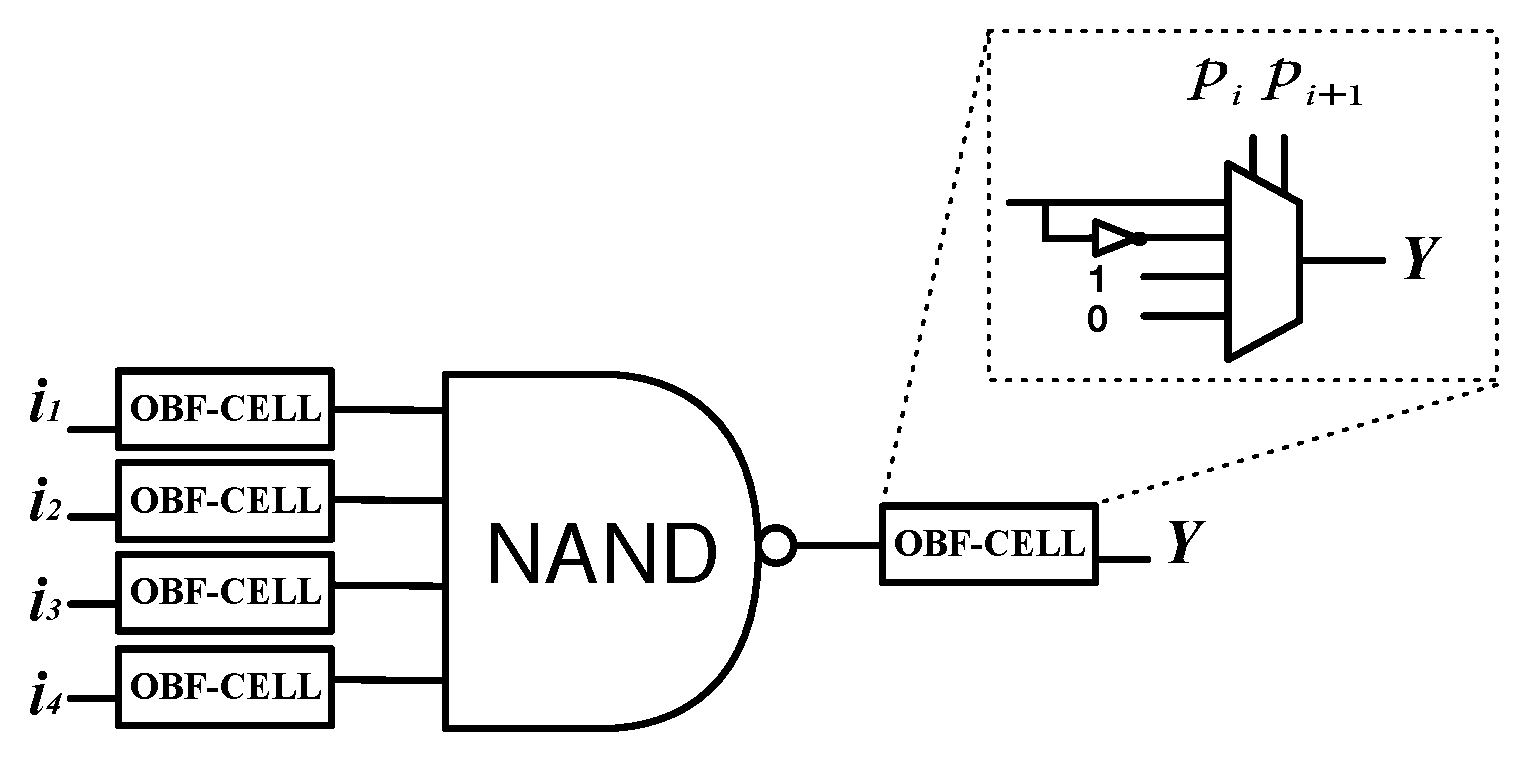
\includegraphics[scale=0.5]{figures/obfus_cell.eps}
\caption{Schematic of a single \textit{Obfusgate} that consists of 5 Obfuscells together with a 4-input NAND gate. This gate can have 162 different logic functions depending on the logical functions realized by each Obfuscell.}
\label{fig:obfuscell}
\end{center}
\end{figure}



















%%%%%%%%%%%%%%%%%%%%%%%%%		Transformable Interconnection		%%%%%%%%%%%%%%%%
\section{Transformable Interconnects}

A third obfuscation technique that we consider is the so-called \textit{transformable interconnects} techniques proposed by Chen et al.~\cite{chen-2015-dummyWire}. This technique uses two types of contacts in interconnects: magnesium (Mg) contacts which are conductors, and magnesium oxide (MgO) contacts which are not conductors. The idea of this approach is that, when an attacker tries to reverse engineer the chip by delayering it, the Mg contacts will oxidize into MgO, and thus all Mg and MgO contacts will appear indistinguishable to the attacker. A reverse engineer inspecting the chip will be able to infer that some of the contacts must have initially been Mg and others must have been MgO, otherwise there would be a single net with multiple driving gates; however, the attacker would not be able to know which were originally Mg, and therefore he must figure this out using input-output examples.


An example of camouflaging using \textit{transformable interconnect} is shown in Figure~\ref{fig:dummywire}. The reverse engineer's view of the circuit is as shown in Fig.~\ref{fig:dummywire}(a), and from this he will infer that d1, d2, and d3 cannot all be true wires. The configurations in Fig.~\ref{fig:dummywire}(b),~\ref{fig:dummywire}(c) and~\ref{fig:dummywire}(d) represent his set of hypotheses for the true connectivity of the circuit. Each one of these would represent the circuit functionality under a single guess about which wire was a non-conducting dummy. The reverse engineer therefore models the transformable interconnect component as shown in Fig.~\ref{fig:dummywire}(e), where the values of $p_0$ and $p_1$ select the true connectivity of the circuit. Now, just as in the previous components, the reverse engineer can use input-output examples from the circuit to infer the values of $p_0$ and $p_1$ and hence resolve the function of the circuit. 


\begin{figure}[t] 
\begin{center}
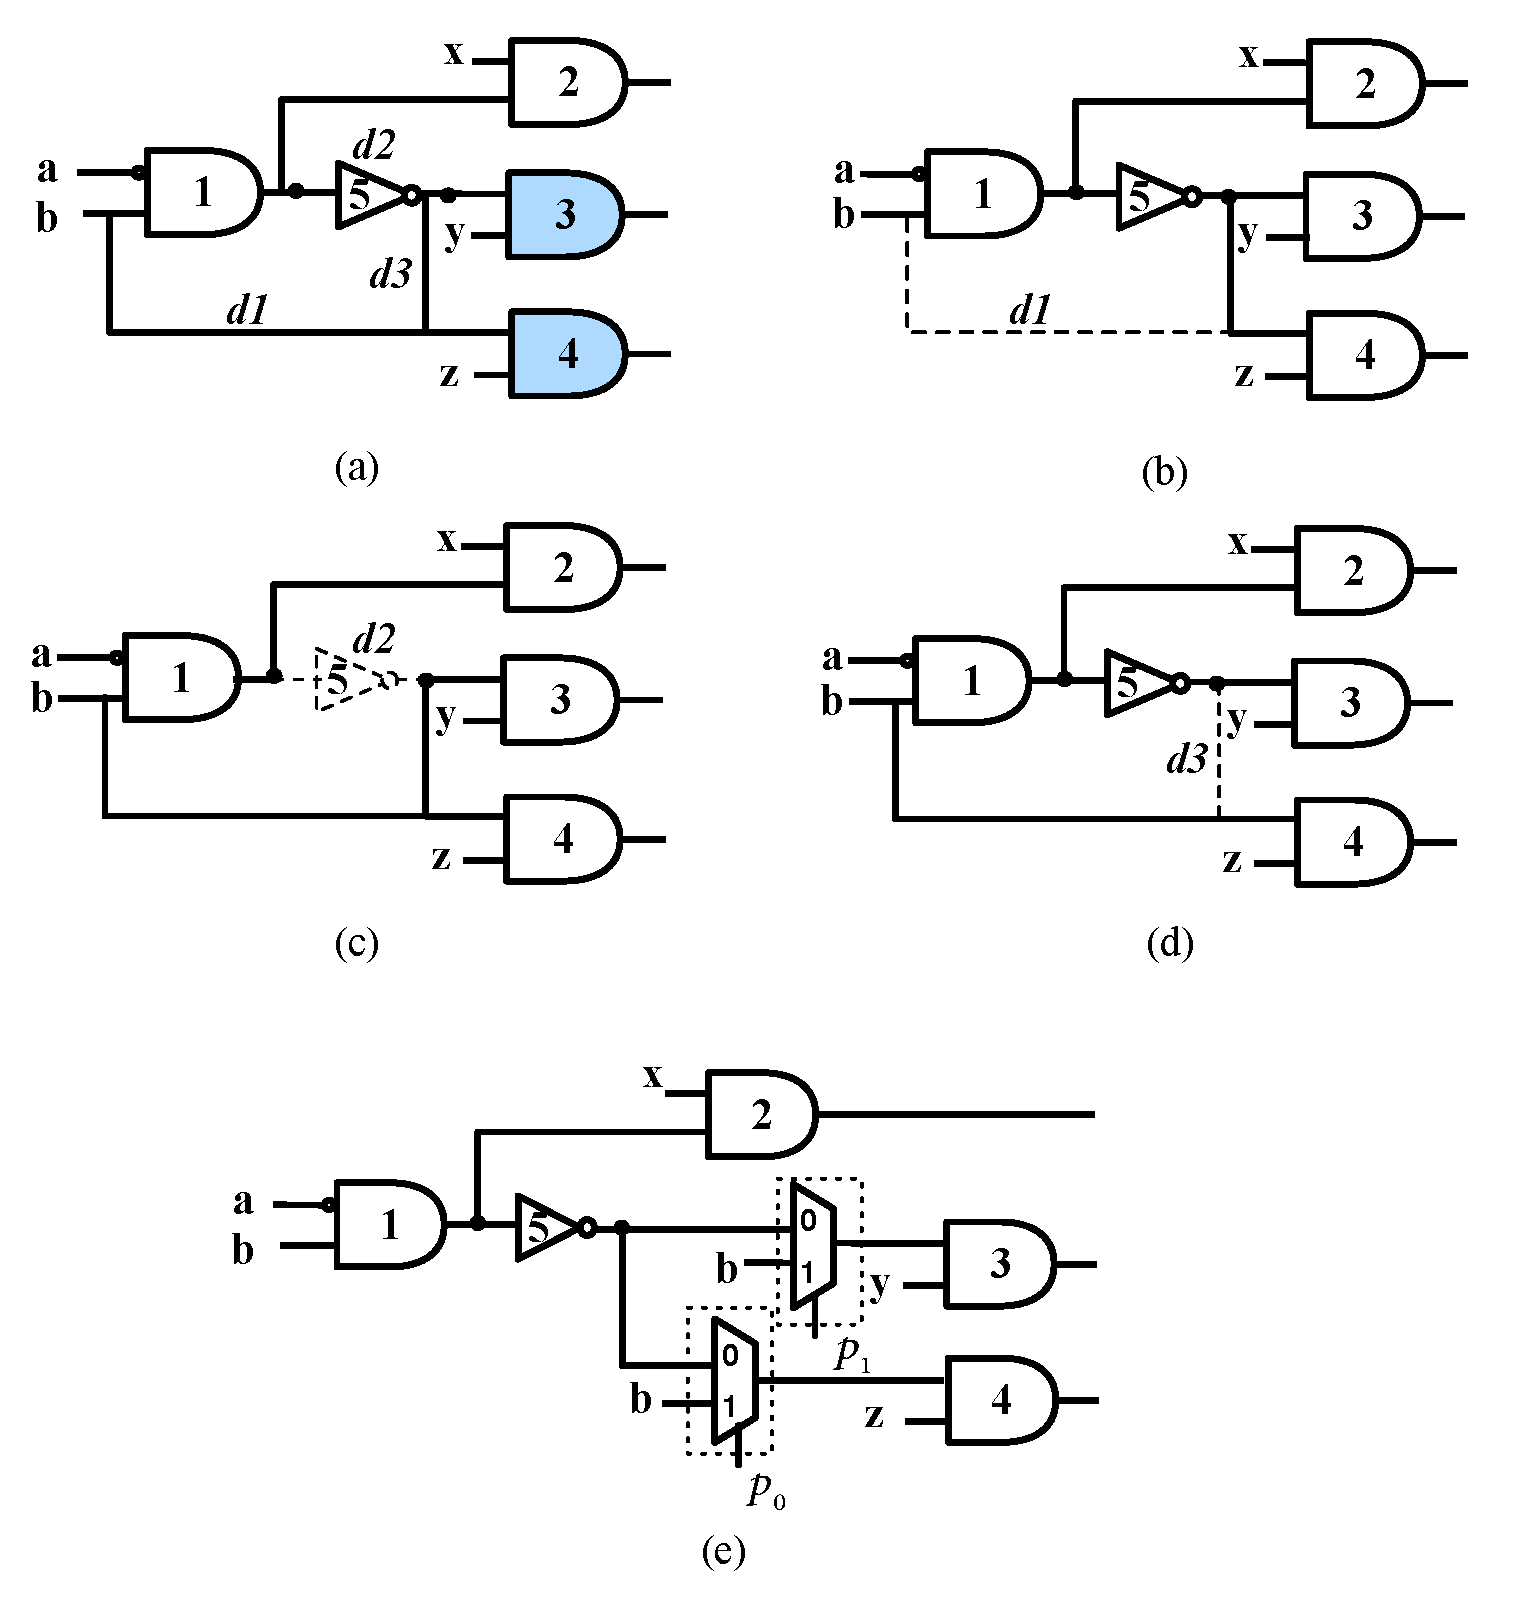
\includegraphics[scale=0.5]{figures/dummywire.eps}
\caption{(a) Design as viewed by reverse engineers; (b, c, d) three valid circuit configurations when $d1$ or $d2$ or $d3$ is transformable interconnect; (e) attacker model of \textit{transformable interconnect}.}
\label{fig:dummywire}
\end{center}
\end{figure}



















%%%%%%%%%%%%%%%%%%%%%%%%%%%%%%%%%%%%%%%%%%%%%%%%%%%%%%%%%%%%%%%%%%%%%%%%%%%%%%%%%%		problem formulation		%%%%%%%%%%%%%%%%%%%%%%%%%%%%%%%%%%%%%%%%%%%%%%%%%%%%%%%%%%%%%%%%%%%%%%%%%%%%%%%%%%%%%%%%
\chapter{problem formulation}

\renewcommand{\algorithmiccomment}[1]{// #1}
\algsetup{indent=2em}
\begin{algorithm*} 
{\fontsize{10}{15}\selectfont
 \begin{algorithmic}[1]
% \footnotesize
\STATE{$M(I, P, P') \gets ckt(I,P,O) \wedge ckt(I,P',O') \wedge O \neq O'$}\label{algline:F} \qquad\qquad\COMMENT{see Fig.~\ref{fig:miter}}
\STATE{$feas(P) \gets \top$} \qquad\qquad\COMMENT{all programming vectors are feasible initially, unless the model itself imposes constraints}
\STATE{$feas(P') \gets \top$}
\FOR{$j=1,2,3\dots$} 

% \STATE{}\COMMENT{num. of sols. to $feas(P)$ is the num. of feasible circuit configurations with respect to I/O pairs 1 to $j$}

% \STATE{}\COMMENT{num. of sols. to $feas(P)$ is the num. of feasible circuit configurations with respect to $(\widehat{I}_1, \widehat{O}_1)$ through $(\widehat{I}_{j-1}, \widehat{O}_{j-1})$}

\STATE{}\label{algline:sharpsat}\COMMENT{{number of satisfying assignments to $feas(P)$ is the number of programming vectors that remain feasible}}

\IF{$ \exists I,P,P'. \ 
\overbrace{  M(I,P,P') }^{I \textnormal{ distinguishes } P \textnormal{ and } P' }
  \wedge 
\overbrace{ feas(P) \wedge feas(P') }^{P \textnormal{ and } P' \textnormal{ both feasible }}
$ } \label{algline:isat1}
\STATE{$\widehat{I}_j \gets I$} 
\STATE{$\widehat{O}_j \gets \textsc{QueryOracle}(\widehat{I}_j)$}\label{algline:oracle}\qquad\qquad\qquad \COMMENT{$(\widehat{I}_j, \widehat{O}_j)$ is the $j^{th}$ I/O pair discovered}
\STATE{$feas(P) \gets feas(P) \wedge ckt(\widehat{I}_j,P,\widehat{O}_j)$} \label{algline:strengthen_p} \quad\quad\COMMENT{strengthen feasibility constraint on $P$ using new I/O pair}
\STATE{$feas(P') \gets feas(P') \wedge ckt(\widehat{I}_j,P',\widehat{O}_j)$} \label{algline:strengthen_pp} \quad\quad\COMMENT{strengthen feasibility constraint on $P'$ using new I/O pair}
\ELSE
\STATE{$ \displaystyle \exists P. feas(P)$ } \label{algline:isat2} \quad\quad \COMMENT{Find a single feasible programming assignment $P$}
\RETURN{$P$}
\ENDIF

\ENDFOR
 \end{algorithmic}
 \caption{{\itshape Incremental SAT-based Deobfuscation:} Incrementally generate a set of constraints that are sufficient to identify the correct model of the circuit, and then solve the constraints to find the model.}
 \label{proc:deobfuscate_incremental}
}\end{algorithm*}



Using the multiplexer-based component models from the previous section (see Figs.~\ref{fig:select}~\ref{fig:obfuscell} and~\ref{fig:dummywire}), we now present a deobfuscation algorithm. The algorithm discovers a programming vector assignment that configures the logic function of the model always to agree with the obfuscated circuit. Discovering such a programming vector is the goal of the attacker, as it deobfuscates the circuit function. He uses known input-output pairings of the circuit {to provide information about} which programming vector values are feasible. A feasible programming vector is one that induces a circuit function that does not contradict any known input-output pairings.

  \begin{figure}[!htb]
  \centering
    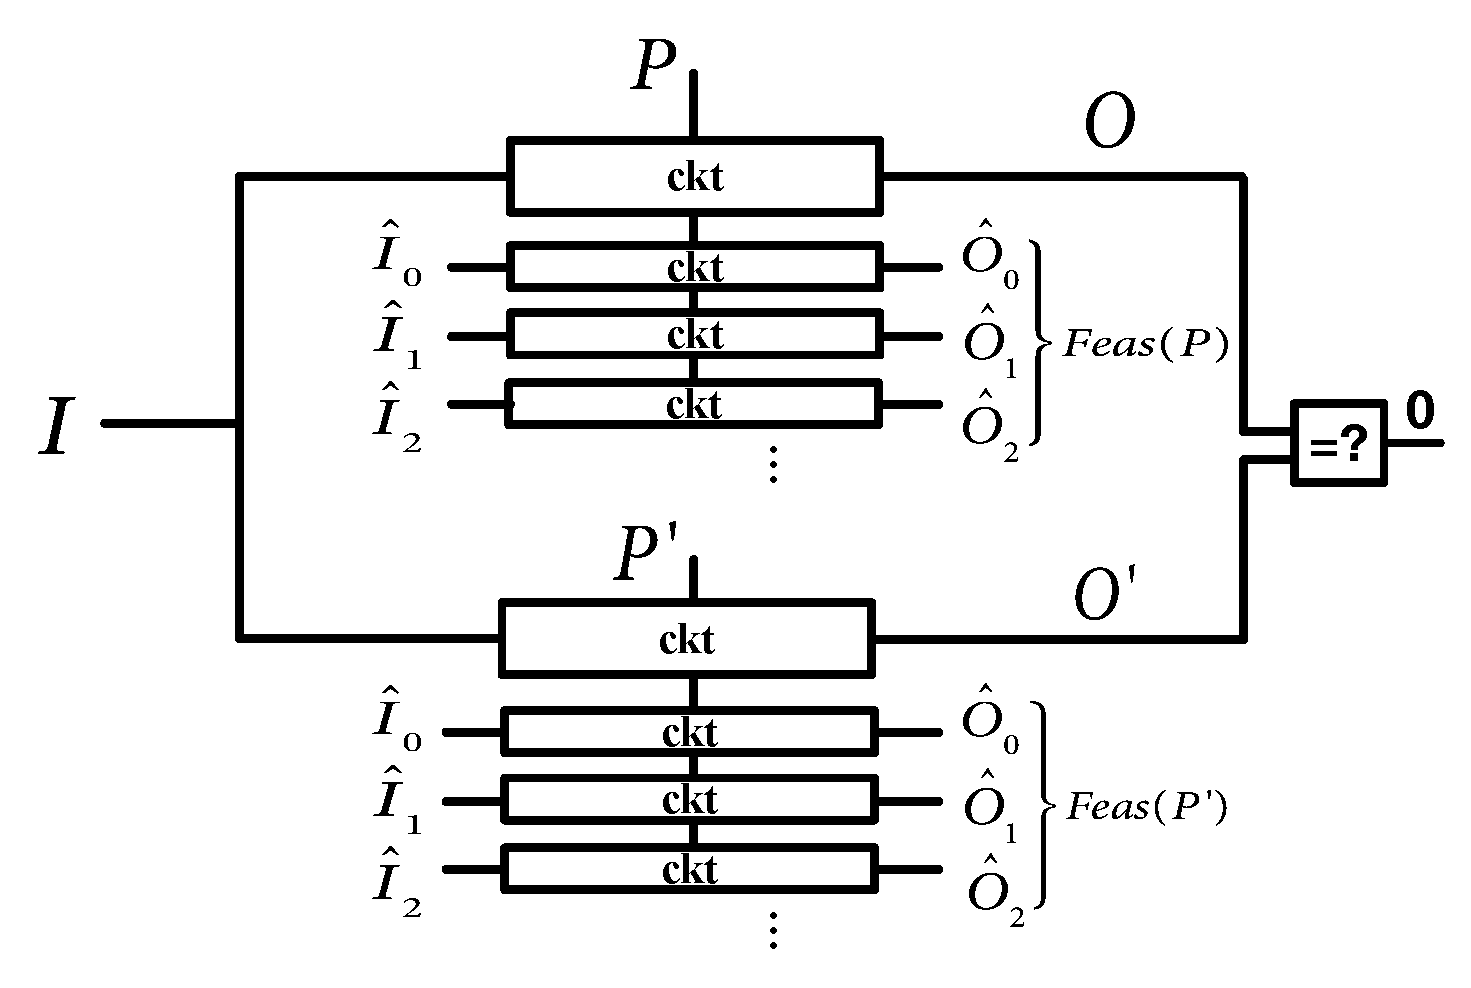
\includegraphics[width=0.7\textwidth]{./figures/miter} 
%    \caption{Two copies of circuit share input vectors but have distinct programming vectors and outputs.}
    \caption{The unshaded components comprise a miter used to find conditions where two copies of the circuit produce different outputs due to different programming vectors. The shaded components enforce feasibility constraints that restrict programming vectors to be consistent with input-output examples.}
    \label{fig:miter}
  \end{figure}

%%%%%%%%%%%%%%%%%%%%%%%%%		Define						%%%%%%%%%%%%%%%%

\section{Defining Notation}
\begin{itemize}

\item Vector $I=\{i_0,\dots, i_{m-1}\}$ represents an $m$-bit primary input vector to the circuit.% ($I \in 2^m$). 

\item Vector $P=\{  p_{0}, p_{1}, \dots \}$ represents a programming vector that specifies the logic function implemented by each camouflaged component in the circuit. The length of the programming vector depends on the number of camouflaged circuit elements and the number of possible realizations for each element. The value of $P$ together with the non-camouflaged circuit components together fully specify the logical function of the overall circuit. We denote a programming vector as \textit{feasible} if the logic function it induces does not contradict a set of known input-output examples. Learning new input-output examples incrementally constrains feasible values of the programming vector $P$.

\item Vector $O=\{o_0,\dots,o_{n-1}\}$ represents an n-bit primary output vector. % ($O \in 2^n$). 

\item The combinational circuit model, including all multiplexers and programming bits, is converted into a CNF formula $ckt$ using Tseitin encoding. We use $ckt(I,P,O)$ to denote the CNF formula of the circuit when $I$, $P$, and $O$ are the input variables, programming bits, and output variables respectively. Wherever $ckt(I,P,O)$ appears in Alg.~\ref{proc:deobfuscate_incremental} (at lines 1, 9, and 10), it always refers to a fresh copy of the circuit CNF with new variables for all internal circuit nodes. If two copies of the circuit CNF share a common input vector or programming vector, the respective inputs or programming vectors are equated to each other outside of the CNF of the combinational circuit. % , the Any logical relationships between different copies of the circuits are will involve only their respective input variables, programming bits, and output variables. 

\item We use subformula $M(I,P,P')$ in Alg.~\ref{proc:deobfuscate_incremental} (line~\ref{algline:F}) to represent the CNF-encoded miter of two copies of the circuit, as shown by the unshaded blocks in Fig.~\ref{fig:miter}. {This formula is satisfiable if and only if there exists an input $I$, and programming vectors $P$ and $P'$ that cause the circuit to map $I$ to different output values. Restated, $M(I,P,P')$ is satisfiable if {\itshape some} $P$ and $P'$ cause the circuit to realize different logic functions. If $M(I,P,P')$ is unsatisfiable, then it means that {\itshape all} $P$ and $P'$ cause the circuit to realize the same logic function. On its own, this formula would typically be easily satisfiable and not meaningful, but it becomes useful when combined with additional feasibility constraints on $P$ and $P'$. In that scenario, the formula $M(I,P,P')$ is used for checking whether the constraints can be satisfied by two different realizable logic functions, or whether the constraints are strong enough that only a single realizable logic function satisfies them. 
%We will show later that these constraints come from $P$ and $P'$ needing be consistent with a set of known input-output examples.
 }


\item {We use subformulas $feas(P)$ and $feas(P')$ to denote the feasibility constraints applied to programming vectors $P$ and $P'$ respectively. These formulas are identical except for being applied to different copies of the programming vector. The formulas evaluate to true only for the subset of programming vectors that are consistent with a set of input-output pairings obtained from the oracle. These feasibility constraints are CNF-encodings of the shaded blocks in Fig.~\ref{fig:miter}}. 


\end{itemize}

The goal of the attacker is to recover the function of the obfuscated circuit by finding a value of $P$ that induces his model to realize the same function as the oracle. Two functions are equivalent if they produce the same outputs for all possible inputs, but equivalence is usually checked symbolically instead of by exhaustively applying inputs. However, symbolic equivalence checking cannot be applied between a model and a black-box oracle, so SAT-based reverse engineering relies on an oracle-guided synthesis approach, as described in the remainder of this paragraph. Given that there are programming vectors to select all possible functions of all camouflaged components, there necessarily exists one or more values of $P$ that will cause the model to realize the same function as the oracle. Because the attacker knows that there must exist such a value of $P$, he can find it by ruling out values of $P$ using input-output examples from the oracle until only a single function remains. At this point, the one function that is not ruled out is known to be equivalent to the oracle by the process of elimination. Any value of $P$ that induces the model to have this function is a solution to the deobfuscation problem.
















%%%%%%%%%%%%%%%%%%%%%%%%%		SAT							%%%%%%%%%%%%%%%%

\section{SAT Solving of Camouflaged circuit}
Boolean satisfiability solving is a common technique for reasoning about circuit logic that is used widely in automated test pattern generation (ATPG)~\cite{larrabee-92}. A gate-by-gate translation using Tseitin encoding maps the circuit logic into a (CNF)-encoded SAT problem. The number of variables in the resulting CNF problem is equal to the number of nodes in the circuit, and the number of clauses in the CNF problem is linear in the number of circuit logic gates. The CNF clauses constrain the Boolean values of the circuit nodes to be consistent the logic gates that relate them. If a CNF problem is satisfiable, a SAT solver finds an assignment of 0 or 1 to each variable that is consistent with the circuit logic gates and any additional constraints added to the problem.

What makes the deobfuscation problem different from ATPG is that obfuscated components are represented by the CNF formula using the circuit constructs of Figs.~\ref{fig:select},~\ref{fig:obfuscell}, and~\ref{fig:dummywire}, which get encoded into the CNF in the same manner as all other nodes and gates. The variables in the CNF problem then include circuit inputs, circuit outputs, and the programming vector. When a known input-output pair is applied to the circuit, unit clauses are added to the CNF to force the appropriate variables to take the desired values. To avoid confusion {with arbitrary input and output vectors ($I$ and $O$ respectively)}, we denote an input-output pairing that is known to be correct as $\widehat{I}$ and $\widehat{O}$ with various subscripts. 















%%%%%%%%%%%%%%%%%%%%%%%%%		Alg							%%%%%%%%%%%%%%%%

\section{Incremental-SAT Algorithm}

Our oracle-guided incremental-SAT based algorithm is given in Alg.~\ref{proc:deobfuscate_incremental}. Following the notation described at the start of this section, the algorithm uses the sub-formula $M(I,P,P')$ to check whether two programming vectors induce different logic functions, and uses $feas(P)$ and $feas(P')$ to constrain programming vector assignments to be consistent with all previously observed input-output pairs. {In Alg.~\ref{proc:deobfuscate_incremental}, both $feas(P)$ and $feas(P')$ are typically initialized to $\top$ meaning that the programming vectors are initially unconstrained; however, when using the modeling construct in Fig.~\ref{subfig:select2} where only the 00,01, and ten values are used for each pair of programming bits, we initialize the constraints to rule out the 11 assignment.}

The feasibility constraints are increasingly strengthened as the algorithm iterates through the loop. At the $j^{th}$ loop iteration in Alg.~\ref{proc:deobfuscate_incremental}, a satisfying assignment at line~\ref{algline:isat1} produces an input vector $I$ that can distinguish two feasible programming vectors $P$ and $P'$. This vector $I$ is assigned to $\widehat{I}_j$ and the oracle is queried to obtain the corresponding output $\widehat{O}_j$. {The pair ($\widehat{I}_j, \widehat{O}_j$) is known to be a correct input-output pairing according to the oracle, and it is used to strengthen the programming vector feasibility constraints at lines~\ref{algline:strengthen_p} and~\ref{algline:strengthen_pp}}. To strengthen the constraints on $P$, a new copy of the circuit CNF formula is added with $P$ as its programming vector and $\widehat{I}_j$ and $\widehat{O}_j$ applied to inputs and outputs as unit clauses (line~\ref{algline:strengthen_p}). The feasibility constraint on $P'$ is strengthened in the same way (line~\ref{algline:strengthen_pp}). {The strengthening of the feasibility constraints corresponds to adding new shaded blocks in Fig.~\ref{fig:miter}. Note that the strengthened feasibility constraints will necessarily have fewer solutions after being strengthened; specifically, among the values $P$ and $P'$ that satisfied the SAT formula at line~\ref{algline:isat1}, at least one will now be infeasible\footnote{Because $P$ and $P'$ induce different outputs under the input vector $\widehat{I}_j$, no more than one of them can induce output vector $\widehat{O}_j$, which is now known to be correct.}.}

Once the feasibility constraints are sufficiently strong, there will no longer exist two different programming vectors that induce distinct logic functions while also satisfying the feasibility constraints. At this point, the SAT call at line~\ref{algline:isat1} becomes unsatisfiable, and a final SAT call is made (line~\ref{algline:isat2}) to find a single programming vector $P$ that satisfies the feasibility constraints. Note that the value of $P$ that is discovered may not be a unique solution, but it is known that no other feasible $P'$ induces a different overall logic function\footnote{If two programming vectors do not produce different outputs for any input vectors, then they induce the same logic function}, as this is necessary for the SAT call at line~\ref{algline:isat1} to be unsatisfiable.

Relative to SAT-based attacks of El Massad et al.~\cite{elmassad-15} and Subramanyan et al.~\cite{subramanyan-15}, a distinguishing feature of our work is the use of incremental SAT. A typical SAT problem is encoded in CNF and solved by a SAT solver to output either a satisfying assignment or a result of \textit{UNSAT} to indicate that no such assignment exists. In the process of solving the SAT problem instance, the solver spends considerable time learning from conflicts and making inferences to simplify the problem and guide its search toward a satisfying assignment. If solving a set of related SAT instances, it is desirable to reuse this reasoning to reduce the number of costly inferences made in each SAT call~\cite{een2003temporal}; incremental SAT is the formulation that allows for efficient reuse of inference across related SAT instances. Our problem is amenable to solving by incremental SAT because each SAT query (line~\ref{algline:isat1} of Alg.~\ref{proc:deobfuscate_incremental}) is solving an instance obtained by adding clauses (at lines~\ref{algline:strengthen_p} and~\ref{algline:strengthen_pp}) to the previously-solved SAT problem instance. All inferences learned in one SAT problem are therefore still applicable in the subsequent one. 

A number of engineering challenges are addressed in order to use an oracle-guided approach with incremental SAT solving. An overview is given here, with more information found in the user manual included with our program. The algorithm is implemented using a modified version of MiniSat~\cite{een-04} version 2.2.0. From within MiniSat, at each iteration of the algorithm, when a satisfying assignment to the CNF is produced (at line~\ref{algline:isat1} of Alg.~\ref{proc:deobfuscate_incremental}), the primary input values ($\widehat{I}_j$) are extracted and mapped into their corresponding signal names and printed to a file. The oracle, implemented as a standalone executable, is then queried (line~\ref{algline:oracle}) and the program waits for the oracle to map $\widehat{I}_j$ to $\widehat{O}_j$. Once the oracle has produced $\widehat{O}_j$, the program adds new clauses to the ongoing CNF problem in order to strengthen the constraints on $P$ and $P'$.

We use the MiniSat 2.2.0 (simp) version because it implements variable elimination and simplification before solving. The overhead cost of performing the simplifications is justified because the simplified constraints are carried forward and used in all future iterations. Because this version of MiniSat can eliminate variables, care must be taken to ``freeze'' certain variables so that they will not be eliminated. In our case, the programming vectors $P$ and $P'$, and the input vector $I$, are frozen. Being frozen means that variables will always remain in the SAT problem, and this makes it possible to read out their values whenever a satisfying assignment is found.


















%%%%%%%%%%%%%%%%%%%%%%%%%		Baseline						%%%%%%%%%%%%%%%%

\section{Baseline SAT-based De-obfuscation Algorithm}
Our SAT formulation is similar to the approach that was first demonstrated by El Massad, Garg, and Tripunitara~\cite{elmassad-15}, and we denote this earlier approach as the baseline algorithm that we compare against. Their algorithm is a significant advancement in reverse engineering, and was able to deobfuscate in minutes problems that would take years to deobfuscate using brute force~\cite{rajendran-13}. Aside from attacking different circuits, the significant difference between our approach and the baseline approach is simply that we use incremental SAT to keep strengthening the feasibility constraints within a single persistent SAT problem. By contrast, the baseline approach treats each iteration of the algorithm as an unrelated SAT problem to solve, and does not carry forward anything learned at previous iterations except for the input-output pairings. Therefore, the baseline algorithm does not carry forward any learned information or simplifications from one iteration to the next. In Sec.~\ref{sec:evaluation} we compare the runtime of our incremental approach to the baseline approach.














%%%%%%%%%%%%%%%%%%%%%%%%%		Illusitive		%%%%%%%%%%%%%%%%

\section{Illustrative}
\begin{figure}[t] 
\begin{center}
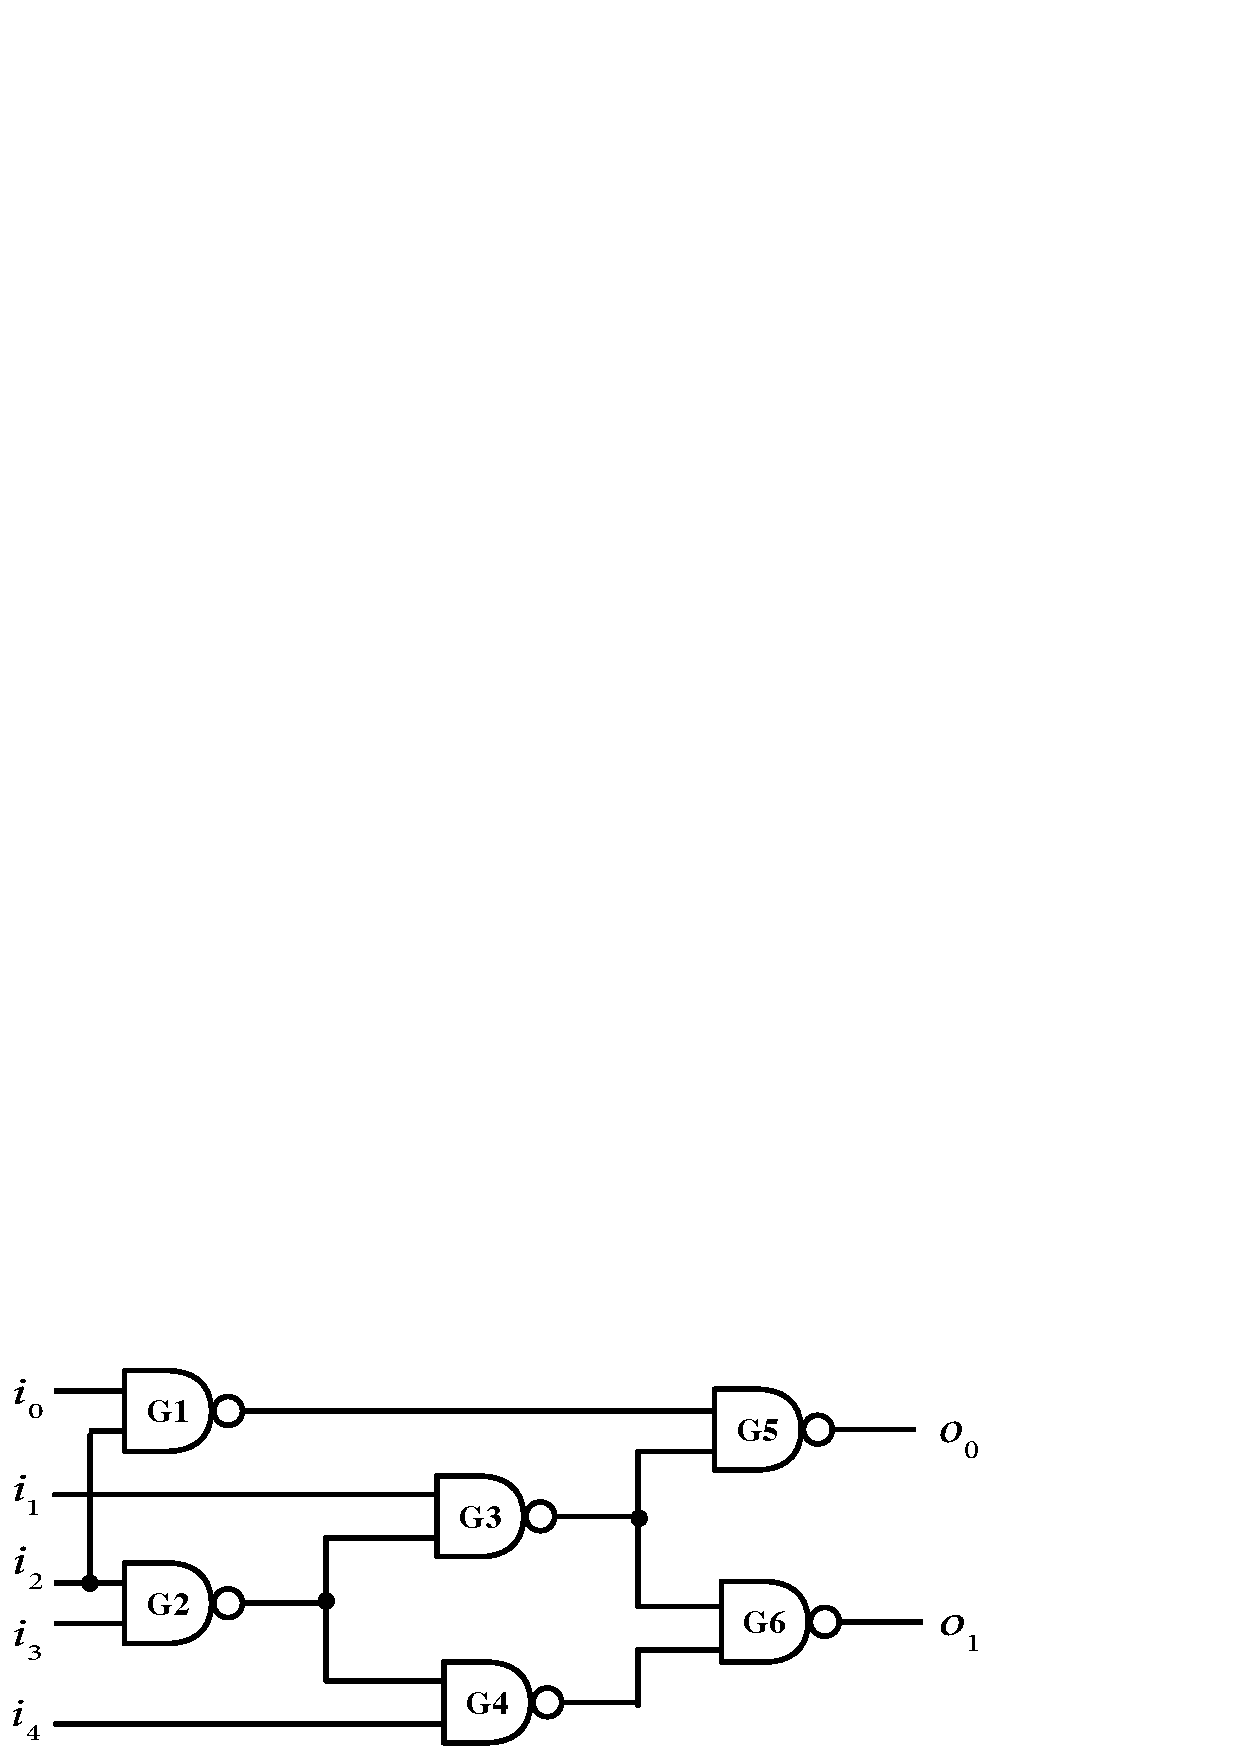
\includegraphics[scale=0.6]{figures/c17_gatelevel.pdf}
\caption{Gate-level netlist of circuit $c17$.}
\label{fig:c17_original}
\end{center}
\end{figure}
%\subsection{Example}

In this section, we demonstrate Alg.~\ref{proc:deobfuscate_incremental} using ISCAS-85 benchmark circuit c17. We demonstrate the algorithm with two types of camouflaging techniques, NAND/NOR/XOR camouflaged standard cells and fully camouflaged logic gates. Additionally, we show an example in which the successfully resolved logic function of the circuit is correct but does not agree with the oracle circuit on a gate-by-gate basis. The gate-level netlist of c17 is shown in Figure \ref{fig:c17_original}.


\subsection{Example 1 - NAND/NOR/XOR Camouflaging}

The NAND/NOR/XOR camouflaged $c17$ circuit is shown in Figure \ref{fig:c17_mux2}. The gates $G{1}$, $G{4}$, and $G{5}$ are camouflaged. We represent the camouflaged gates using the model given in Figure \ref{fig:select}(a). The value of the programming vector $P$ is returned at the end of our algorithm, and this programming vector will select gate functions that make the model logically equivalent to the oracle. For the two bits of the programming vector corresponding to each gate, a value of 00 selects an XOR gate, a value of 01 selects a NAND gate, and a value of 10 selects a NOR gate. Because there are only three possible gate functions, a constraint is added to rule out the value 11 for each pair of programming bits.

The results of each iteration of Alg.~\ref{proc:deobfuscate_incremental} when applied to this example are recorded in Table~\ref{tbl:mux2_solving}. In the table, $j$ is the iteration number; $I$, $P$, $P'$ are the assigned values in the solution to the SAT call at line~\ref{algline:isat1} of the algorithm; ($\hat{I_{j}}$, $\hat{O_{j}}$) are the input-output pairs obtained and used to strengthen feasibility constraints at lines~\ref{algline:strengthen_p}~and~\ref{algline:strengthen_pp} of the algorithm. For example, the first iteration finds input value $I$ = $01000$ which is then applied to the oracle to obtain the input-output pairing ($01000$,$11$). This one pairing reduces the number of feasible programming vectors from 27 to 14. After finding six input-output pairings, on the seventh iteration the SAT call at line~\ref{algline:isat1} becomes unsatisfiable, indicating that the feasibility constraints imposed by these six pairs are sufficient to identify a unique logic function that matches the oracle and thus deobfuscates the circuit. In this example, there is only one feasible configuration remaining at the \textit{UNSAT} iteration. Note that there are usually many feasible configurations remaining at the \textit{UNSAT} iteration on large circuits. Although not depicted in Table~\ref{tbl:mux2_solving}, a final SAT call (line~\ref{algline:isat2} of Alg.~\ref{proc:deobfuscate_incremental}) produces the programming vector $P$ = $010101$ which selects the NAND functionality for gates $G1$, $G4$, and $G5$. This programming vector deobfuscates the circuit, and in this case it happens to do so in a way that is gate-by-gate logically equivalent to the camouflaged circuit. Note in Table~\ref{tbl:mux2_solving} that the number of clauses and unresolved variables at each iteration of the algorithm are growing sub-linearly and sometimes decreasing. This reflects the solving making simplifications to the problem as it runs. This becomes crucially important for large camouflaged designs.

\begin{figure}[!htb] 
\begin{center}
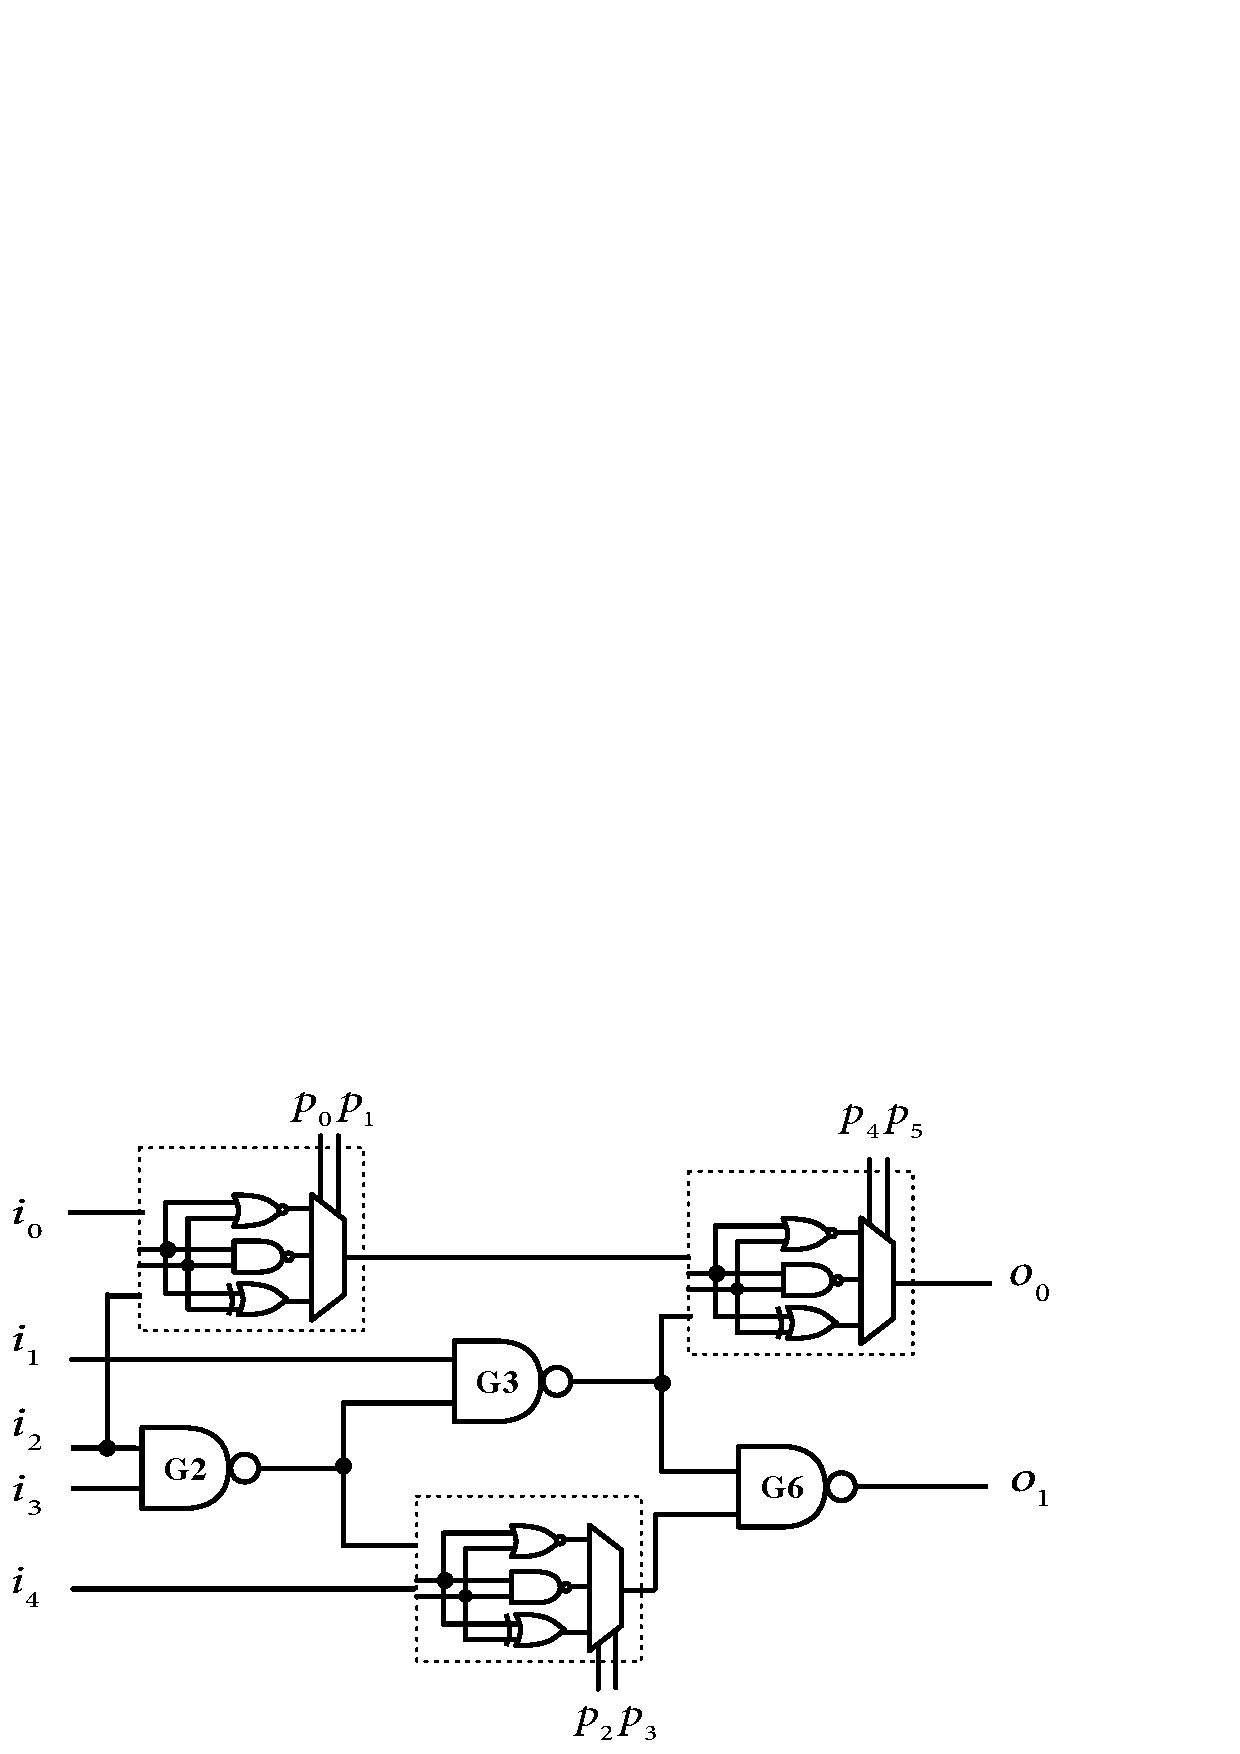
\includegraphics[scale=0.45]{figures/c17_mux2_gatelevel.pdf}
\caption{Modeling of $c17$ benchmark with G1, G4, G5 camouflaged using NAND/NOR/XOR camouflaging.}
\label{fig:c17_mux2}
\end{center}
\end{figure}

\begin{figure}[!htb] 
\begin{center}
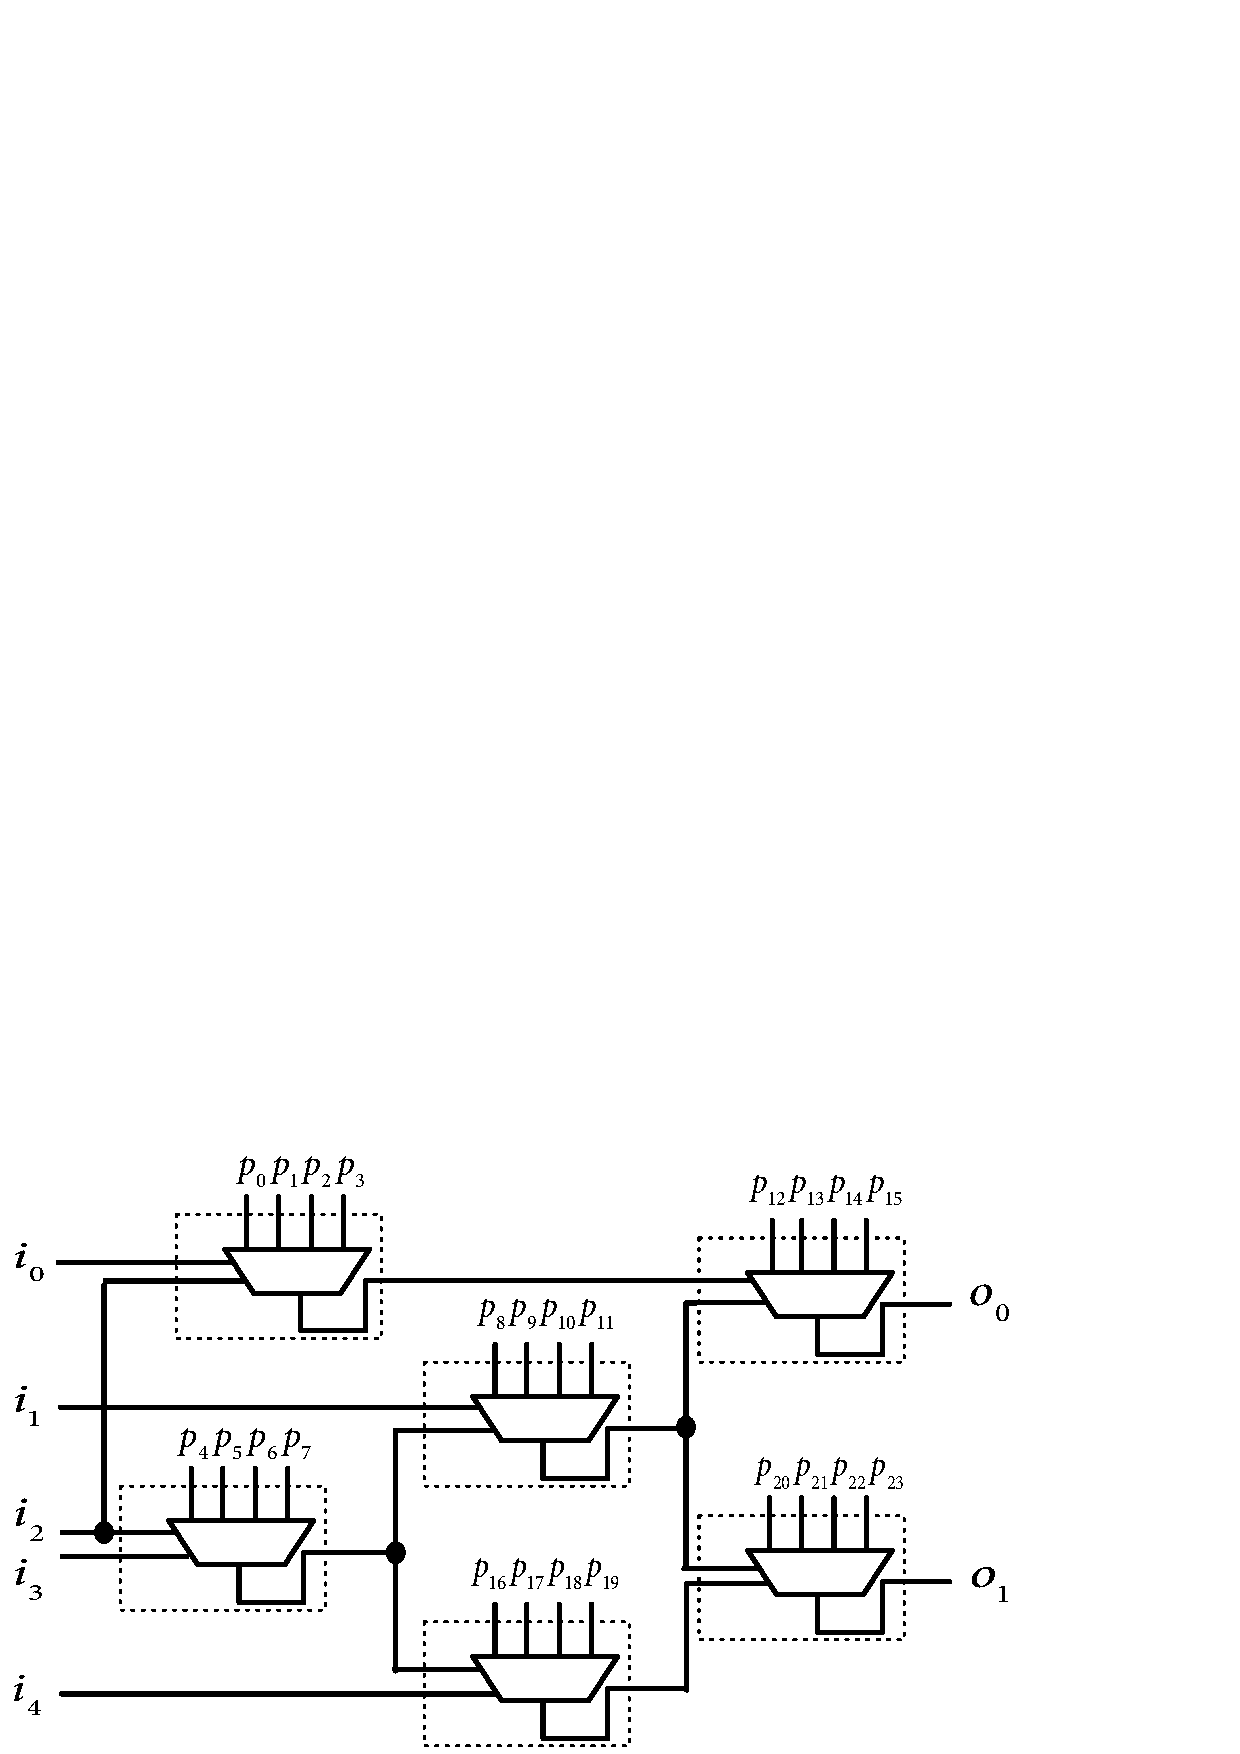
\includegraphics[scale=0.45]{figures/c17_mux4_gatelevel.pdf}
\caption{Modeling of $c17$ with all gates fully camouflaged. In this scenario, the reverse engineer only knows the routing.}
\label{fig:c17_mux4}
\end{center}
\end{figure}



\subsection{Example 2 - All Gates are Camouflaged}

The most challenging case for our algorithm is deobfuscating a circuit in which all the logic gates are fully camouflaged. In this scenario, only the routing is known to the reverse engineer. We demonstrate this problem using $c17$, modeled as shown in Fig.~\ref{fig:c17_mux4}. Our algorithm requires 24 iterations to deobfuscate this small circuit. It is notable that the resolved circuit (Fig.~\ref{fig:c17_all}) is not gate-by-gate equivalent to the obfuscated circuit, but nonetheless has resolved the correct function for the circuit. Deobfuscation when only routing is known does not scale well because the reverse engineer has very little useful information. For example, we are not able to deobfuscate ISCAS benchmark circuit $c432$ after 3 days when all 160 gates are camouflaged in this manner\footnote{The ISCAS-85 benchmark $c432$ has 160 gates, some of which have more than 2 inputs. Because we use 2-input obfuscated gates, we map $c432$ into a circuit with 209 gates of 2 or fewer inputs, and then obfuscate all 209 cells of the remapped circuit.}.


\begin{figure}[htb] 
\begin{center}
%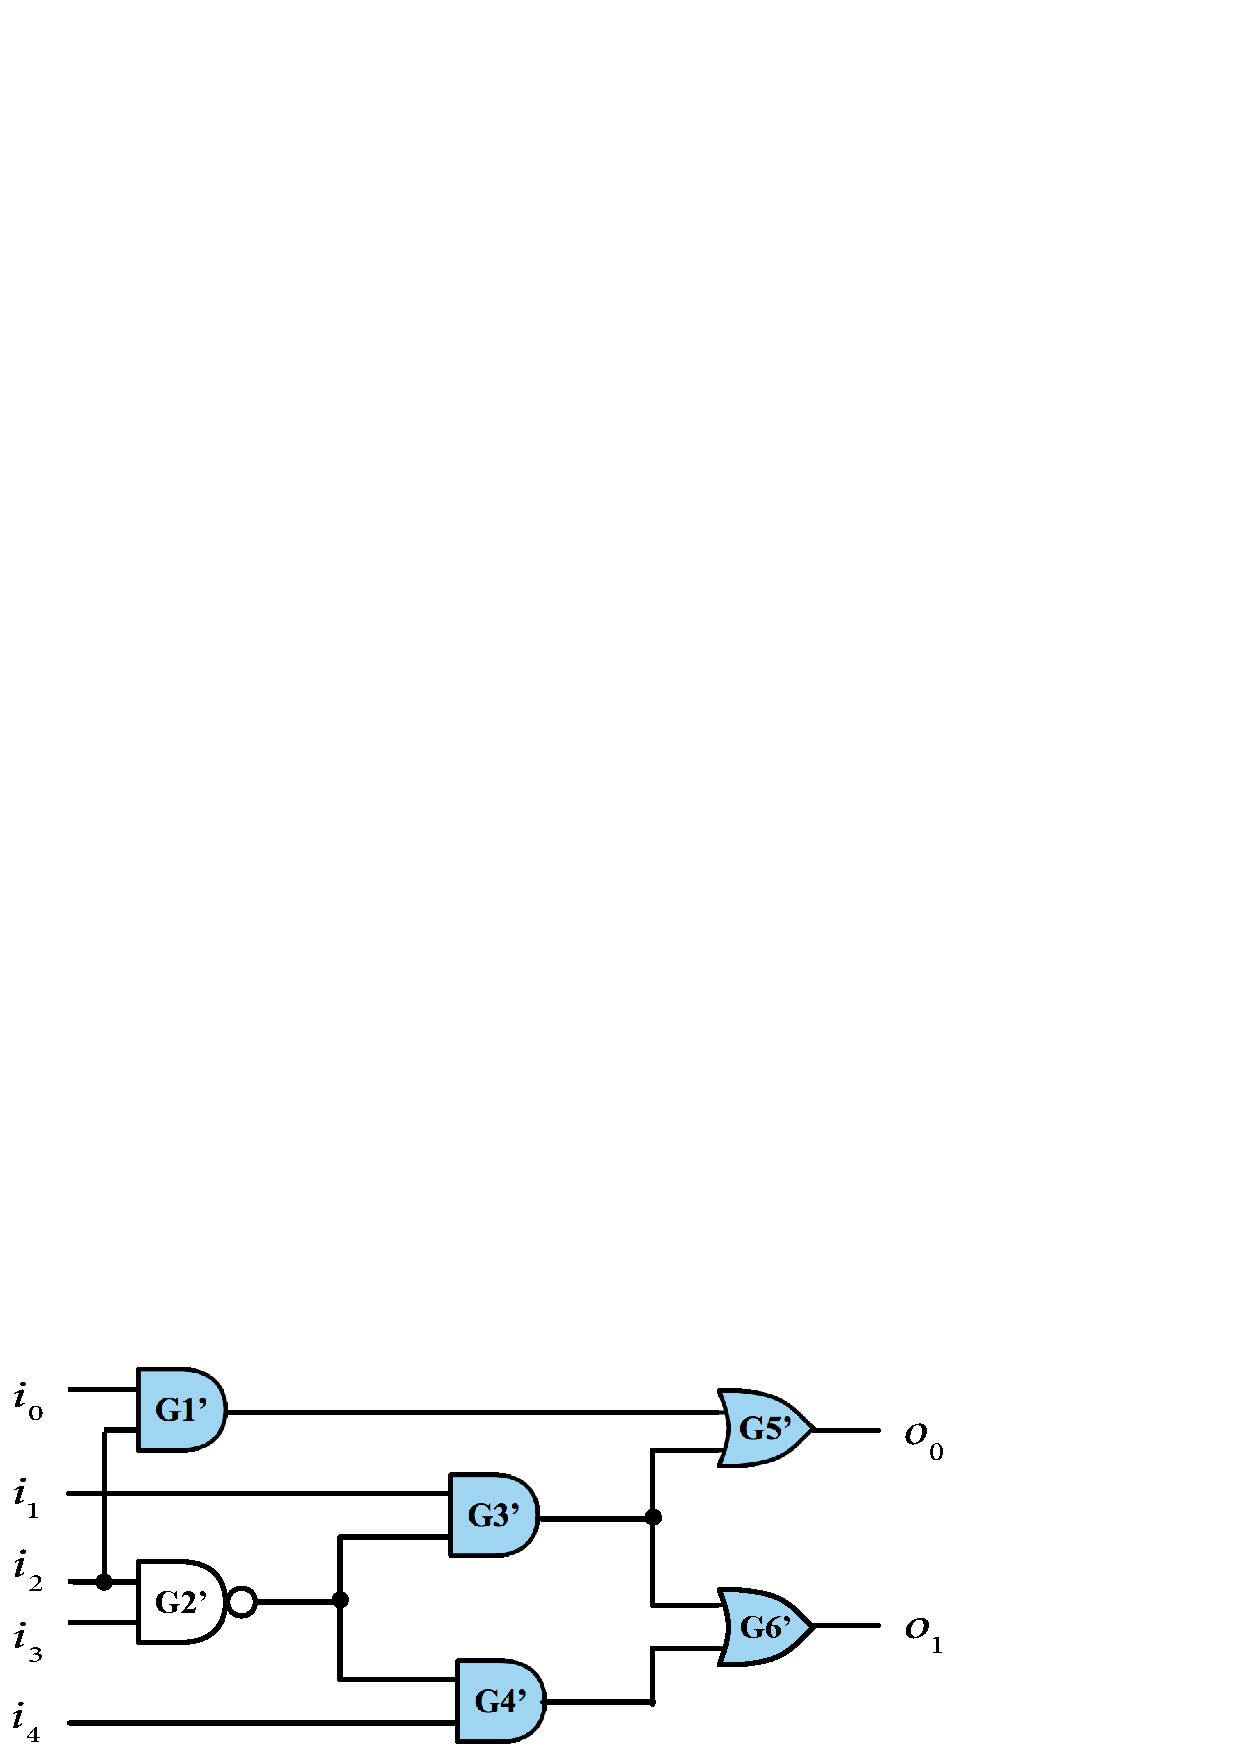
\includegraphics[scale=0.45]{figures/c17_all_camouflage.pdf}
\caption{Resolved function of $c17$ when all gates are fully camouflaged.}
\label{fig:c17_all}
\end{center}
\end{figure}








%%%%%%%%%%%%%%%%%%%%%%%%%%%%%%%%%%%%%%%%%%%%%%%%%%%%%%%%%%%%%%%%%%%%%%%%%%%%%%%%%%		Eva of De-obf		%%%%%%%%%%%%%%%%%%%%%%%%%%%%%%%%%%%%%%%%%%%%%%%%%%%%%%%%%%%%%%%%%%%%%%%%%%%%%%%%%%%%%%%%
\chapter{Evaluation of De-Obfuscation Algorithm}
We evaluate our deobfuscation algorithm on a set of ISCAS-85 combinational benchmarks~\cite{hansen-99} including \textit{c432}, \textit{c499},  \textit{c880}, \textit{c1355}, \textit{c1908}, \textit{c2670}, \textit{c3540},  \textit{c5315}, and \textit{c7552}. The sizes of these circuits range from several hundred to several thousand gates. We use the attacker model introduced in Section 3. Our previous work~\cite{duo-date16} demonstrated that our algorithm is able to efficiently deobfuscate the six largest ISCAS benchmarks with up to 200 gates implemented using NAND/NOR/XOR camouflaged standard cells. %camouflaged in a way that each gate could implement NAND, NOR, or XOR. %For generality, 10 trials are used with different random choices of gates to camouflage; error bars show the ranges of the results across the 10 trials. 








%%%%%%%%%%%%%%%%%%%		Eva of Cam			%%%%%%%%%%%%%%%%%%%%%%%%%%
\section{Evaluation of Camouflaging Techniques}

\begin{figure*}[!hbt]
  \centering
    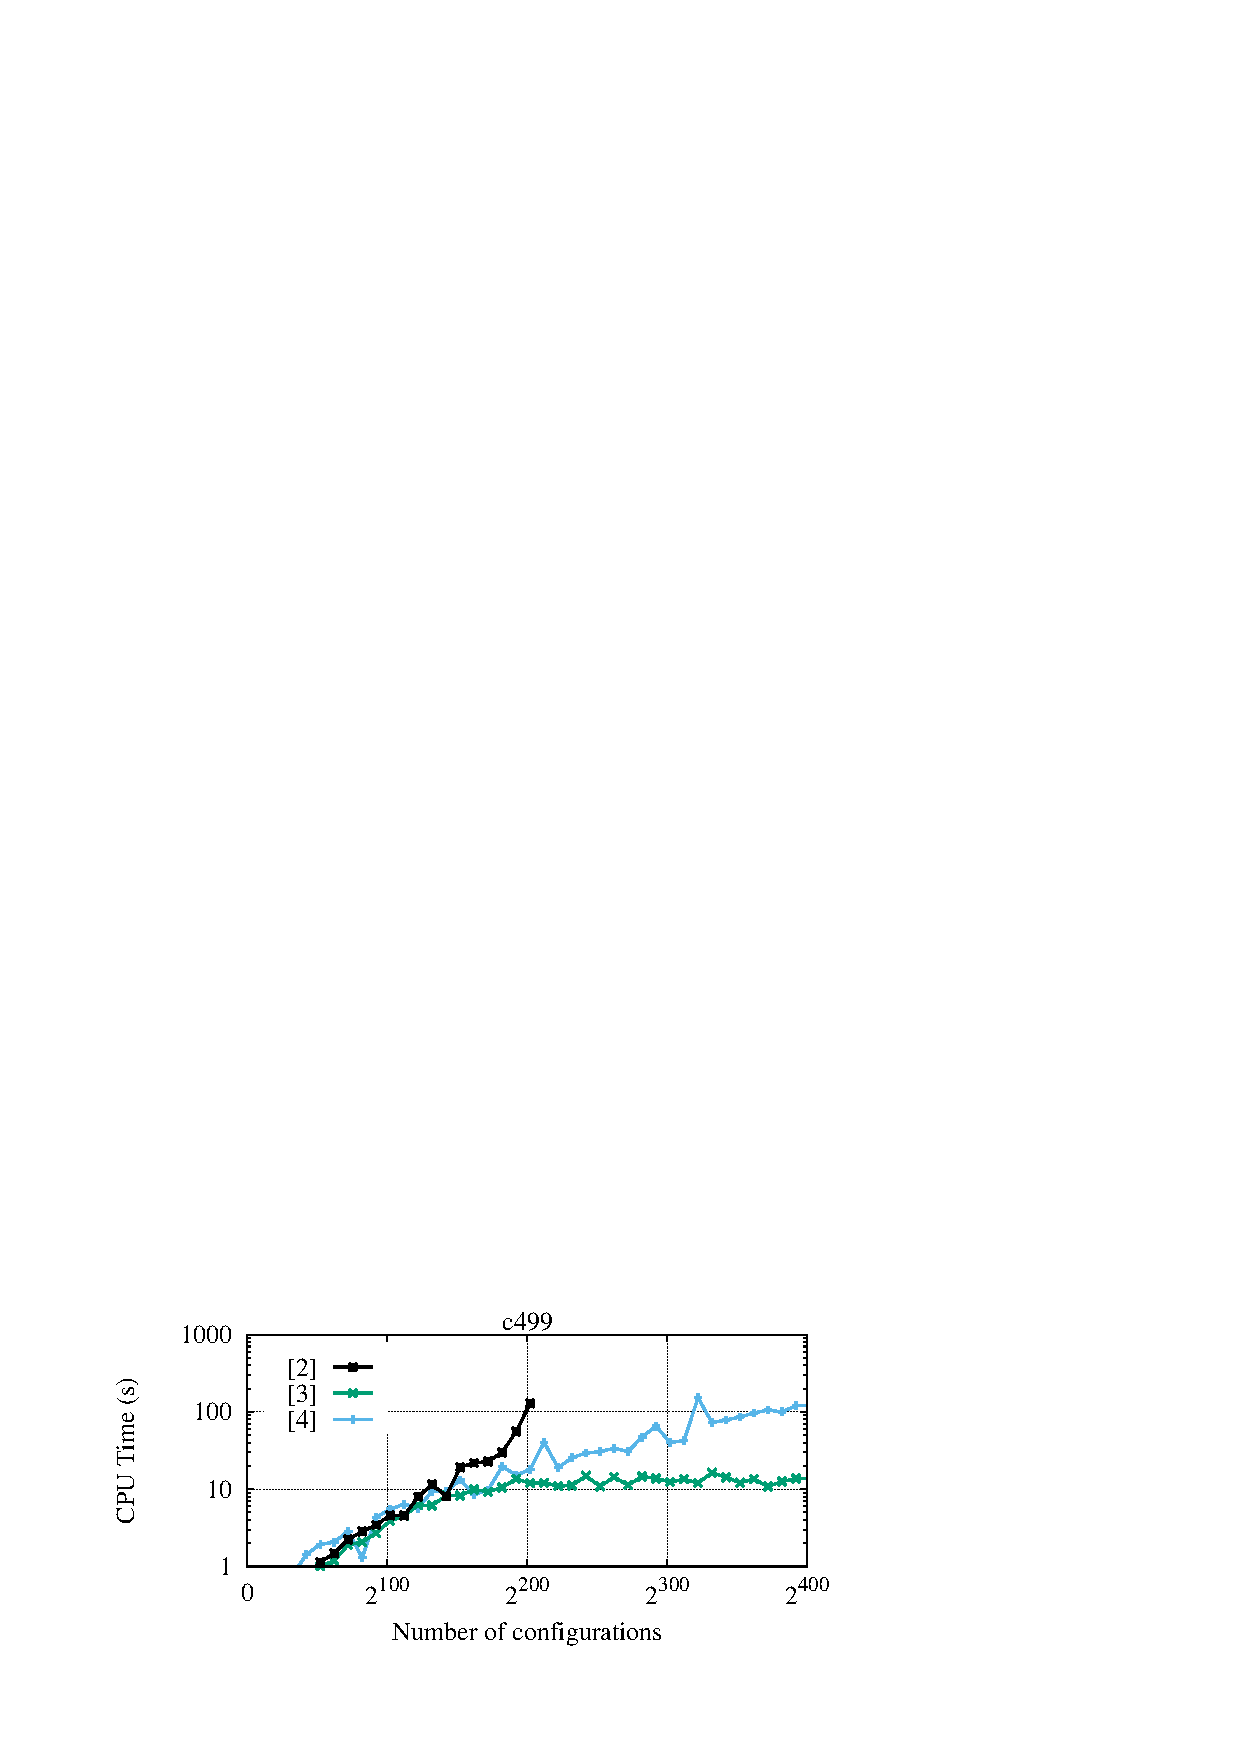
\includegraphics[width=0.48\textwidth]{newdata-tcad16/c499.pdf} \hspace{.3cm}
    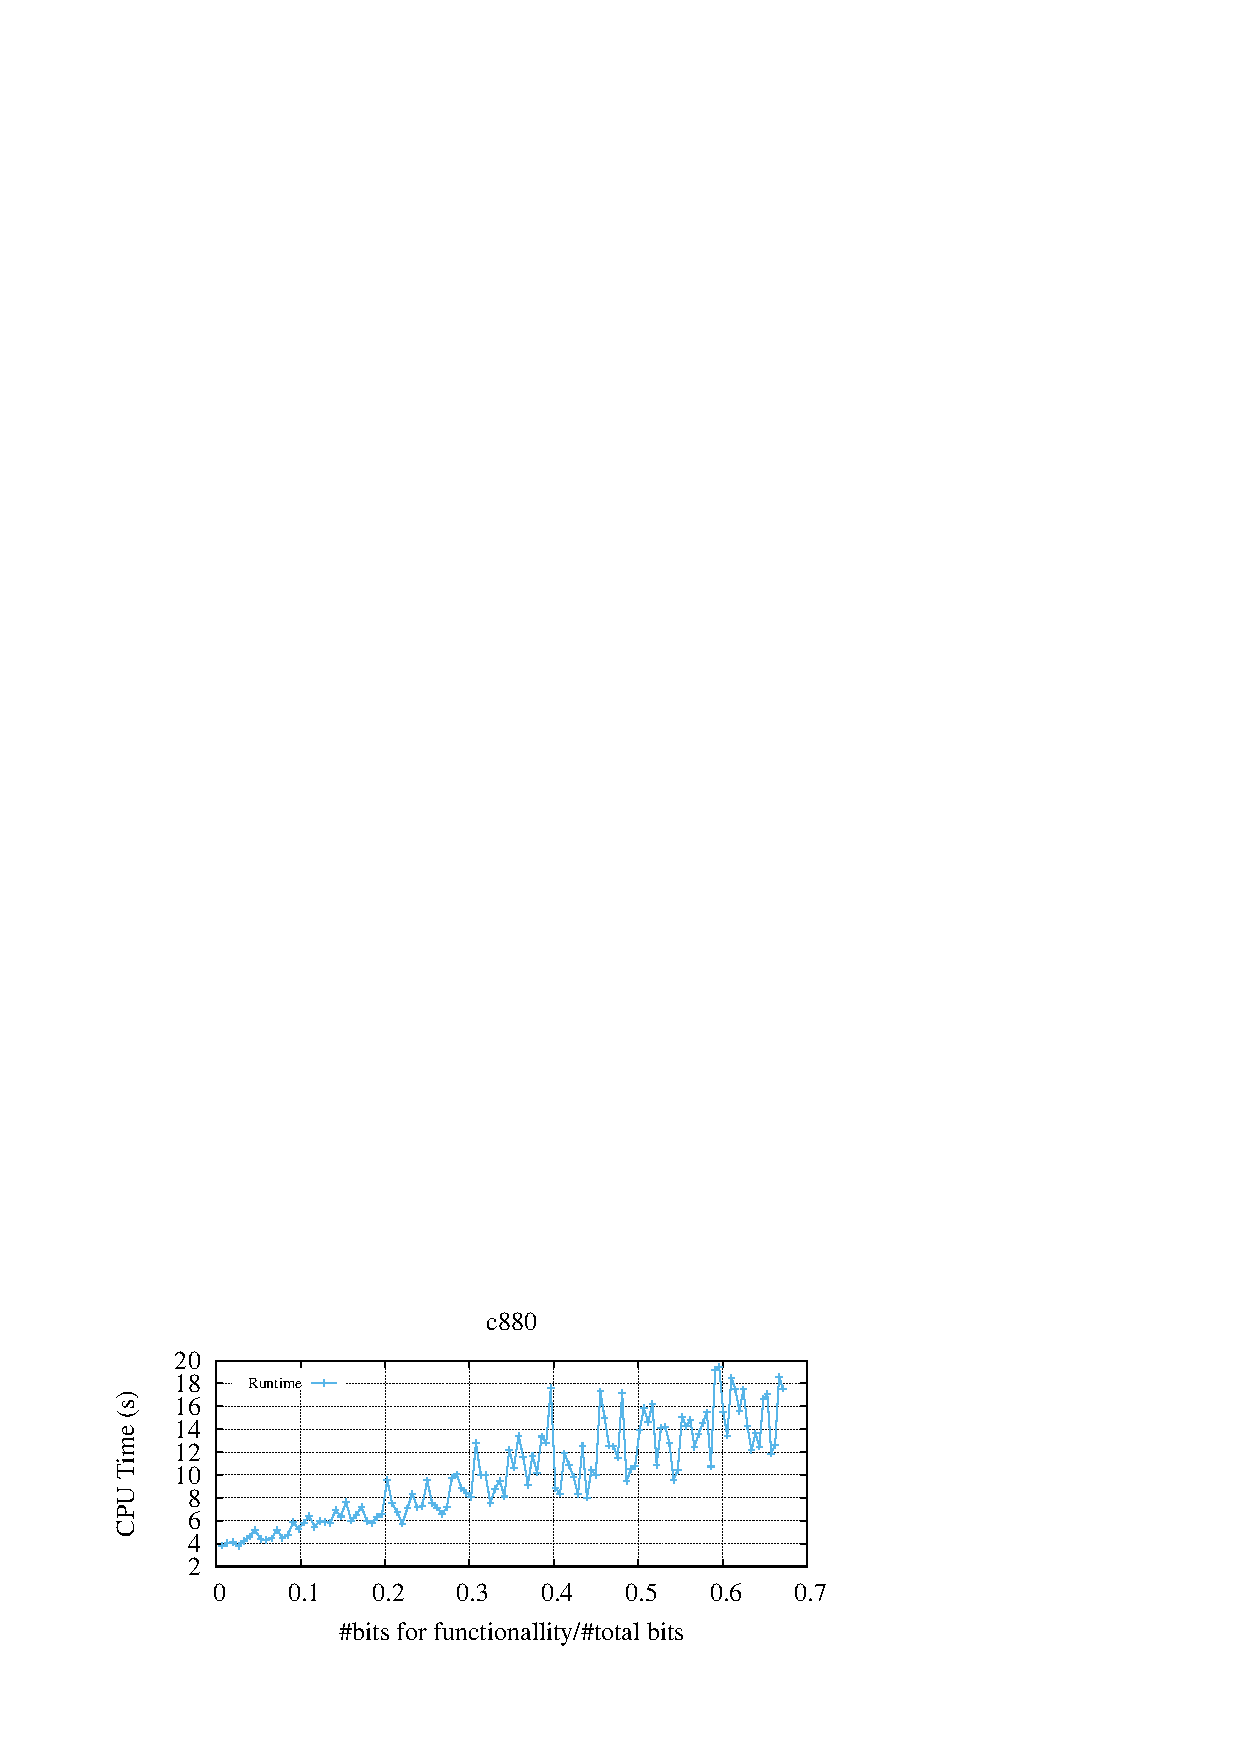
\includegraphics[width=0.48\textwidth]{newdata-tcad16/c880.pdf} 
    \vspace{-2mm}

    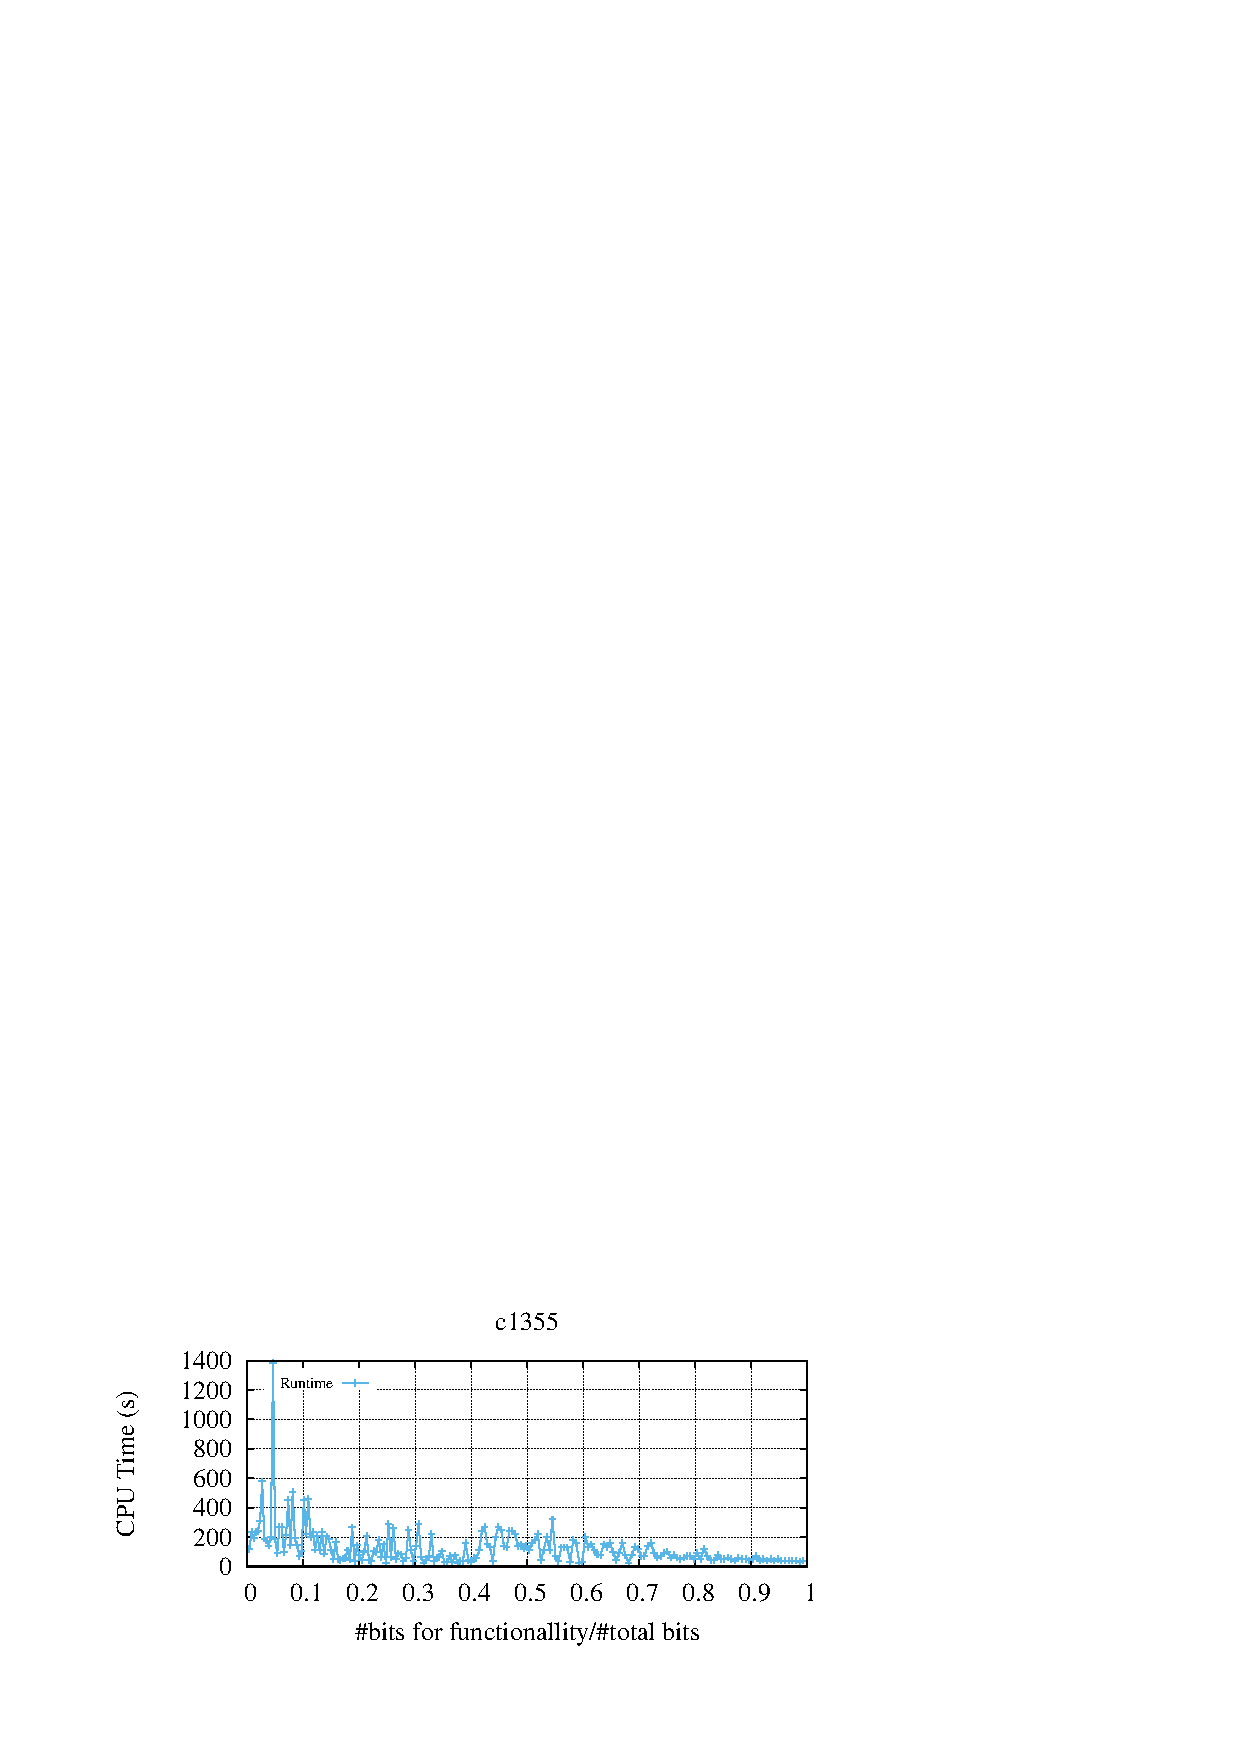
\includegraphics[width=0.48\textwidth]{newdata-tcad16/c1355.pdf} \hspace{.3cm}
    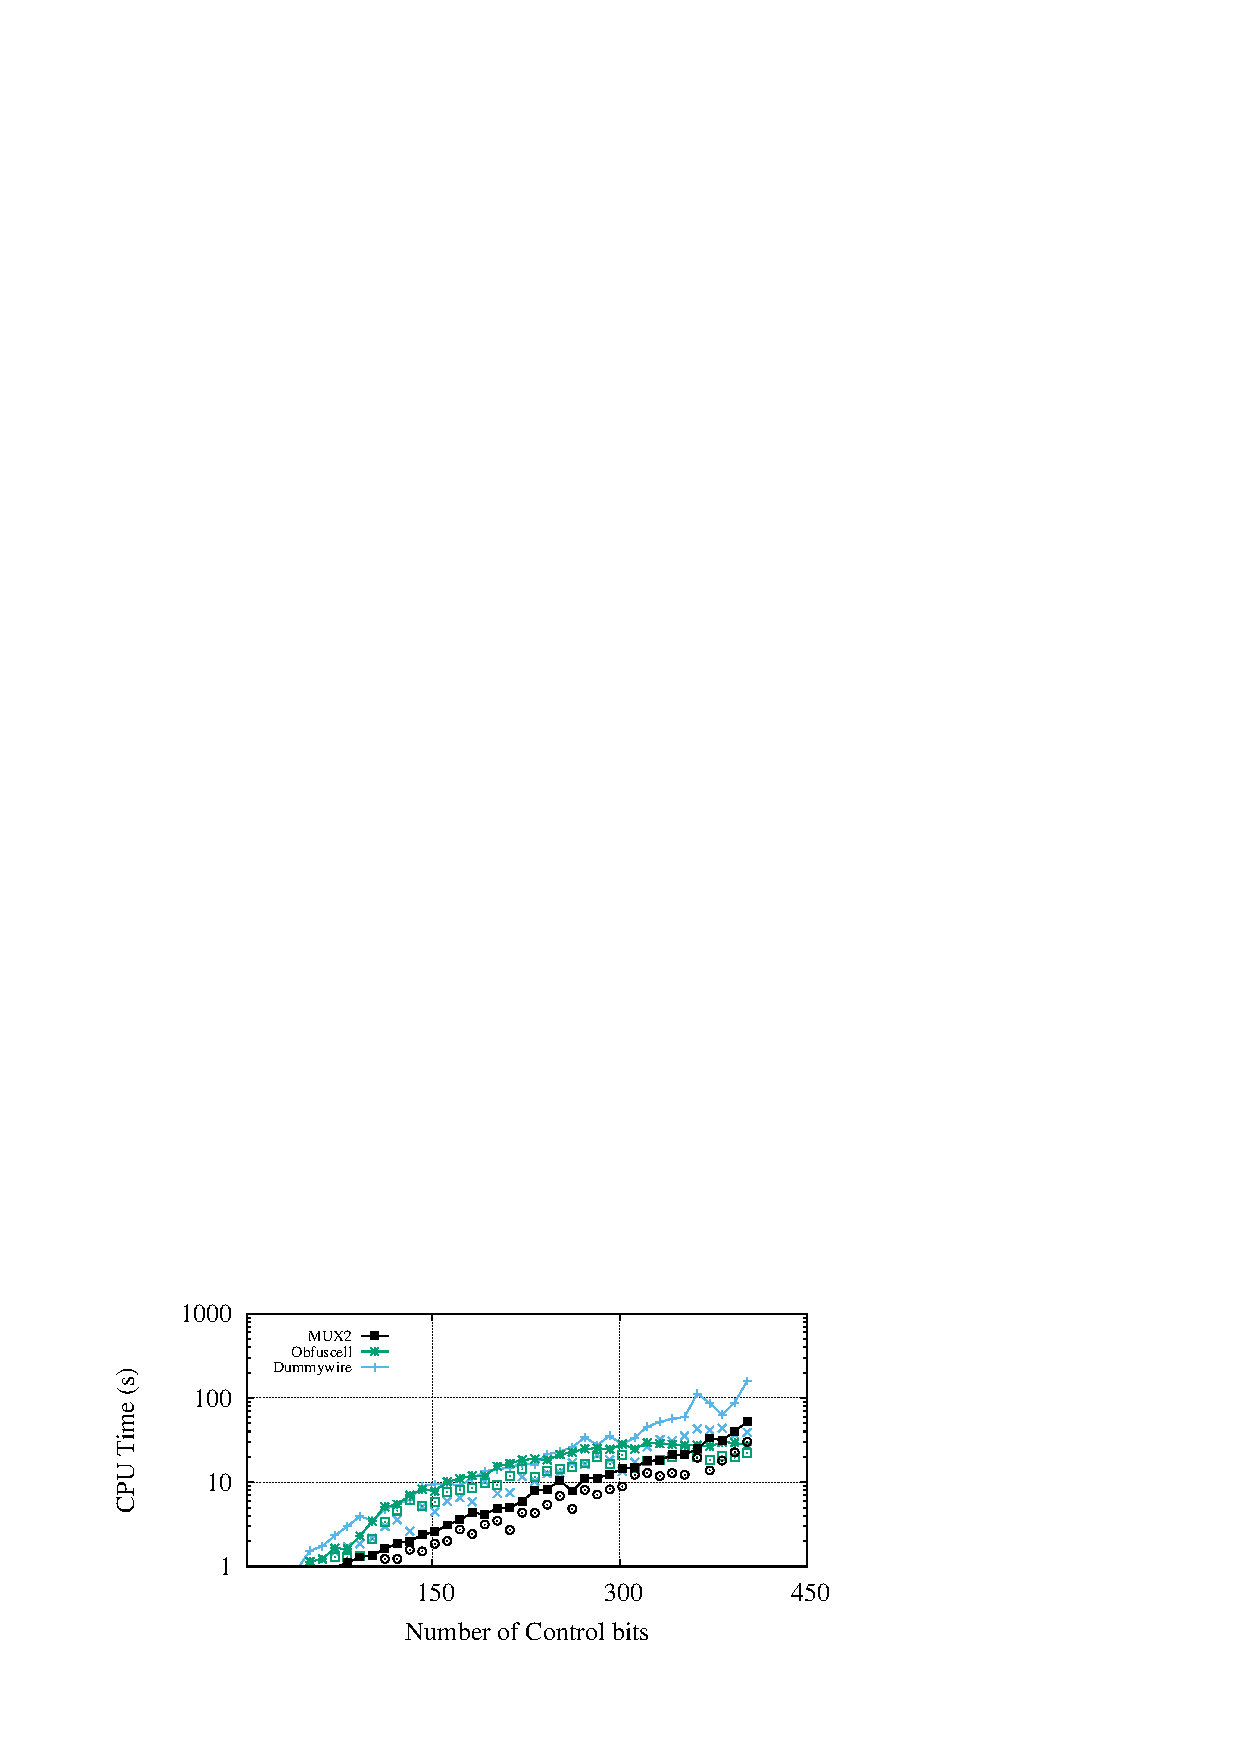
\includegraphics[width=0.48\textwidth]{newdata-tcad16/c1908.pdf} 
        \vspace{-2mm}

    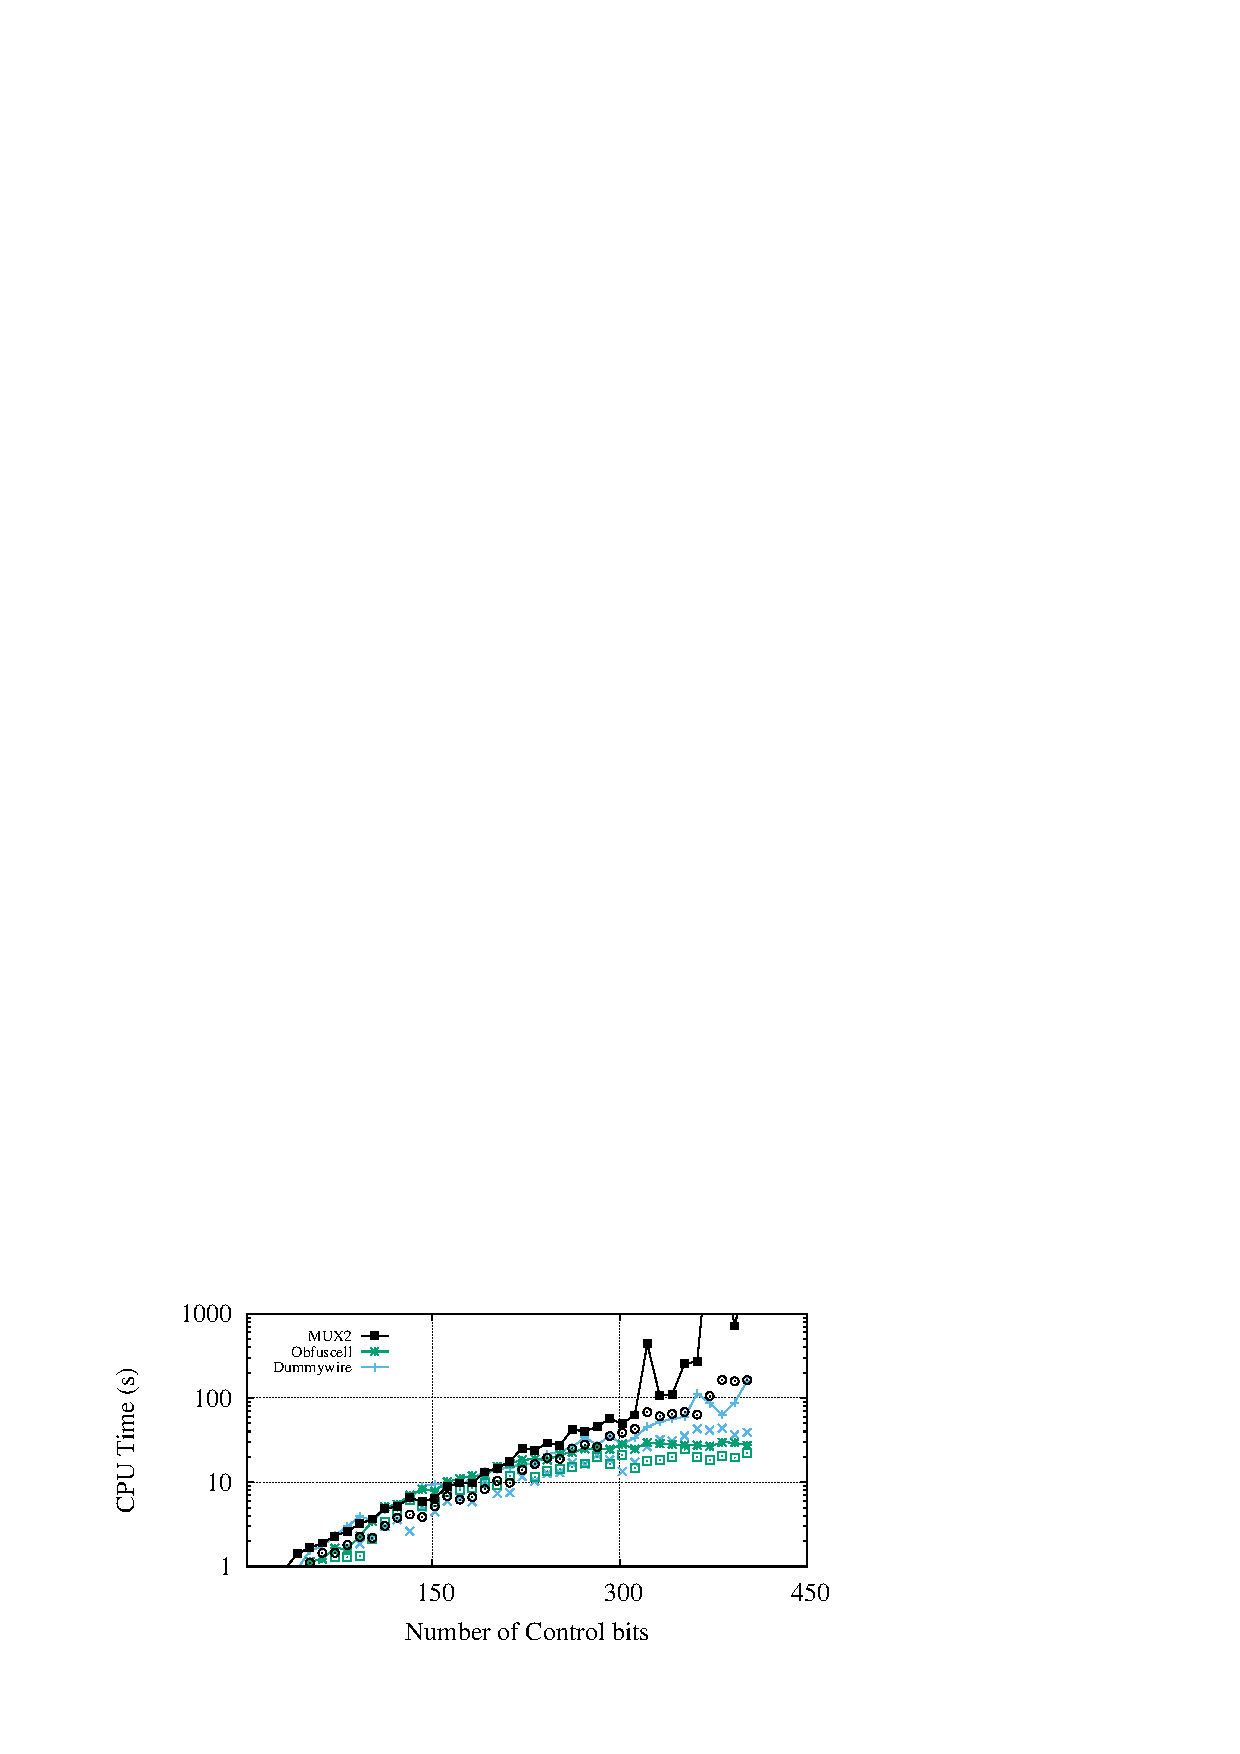
\includegraphics[width=0.48\textwidth]{newdata-tcad16/c2670.pdf} \hspace{.3cm}
    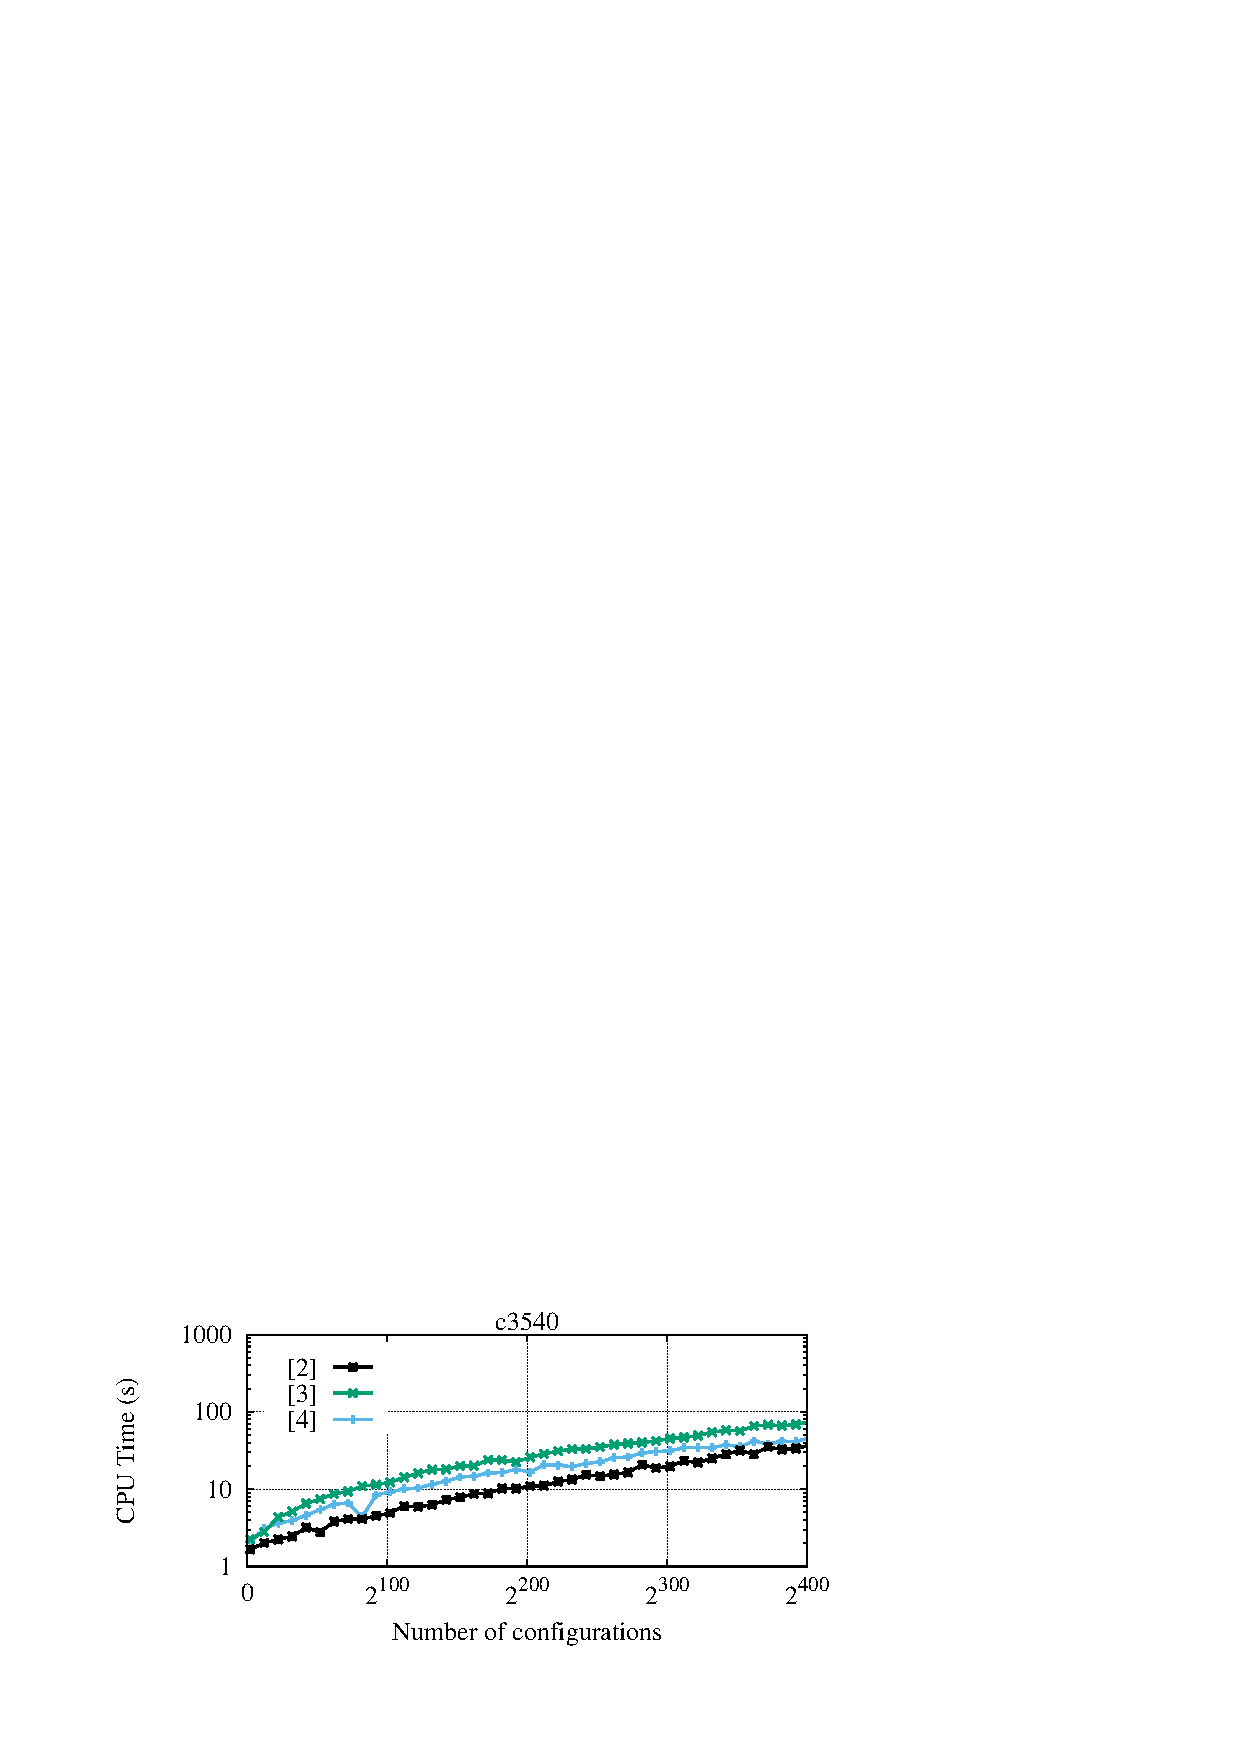
\includegraphics[width=0.48\textwidth]{newdata-tcad16/c3540.pdf}
        \vspace{-2mm}

    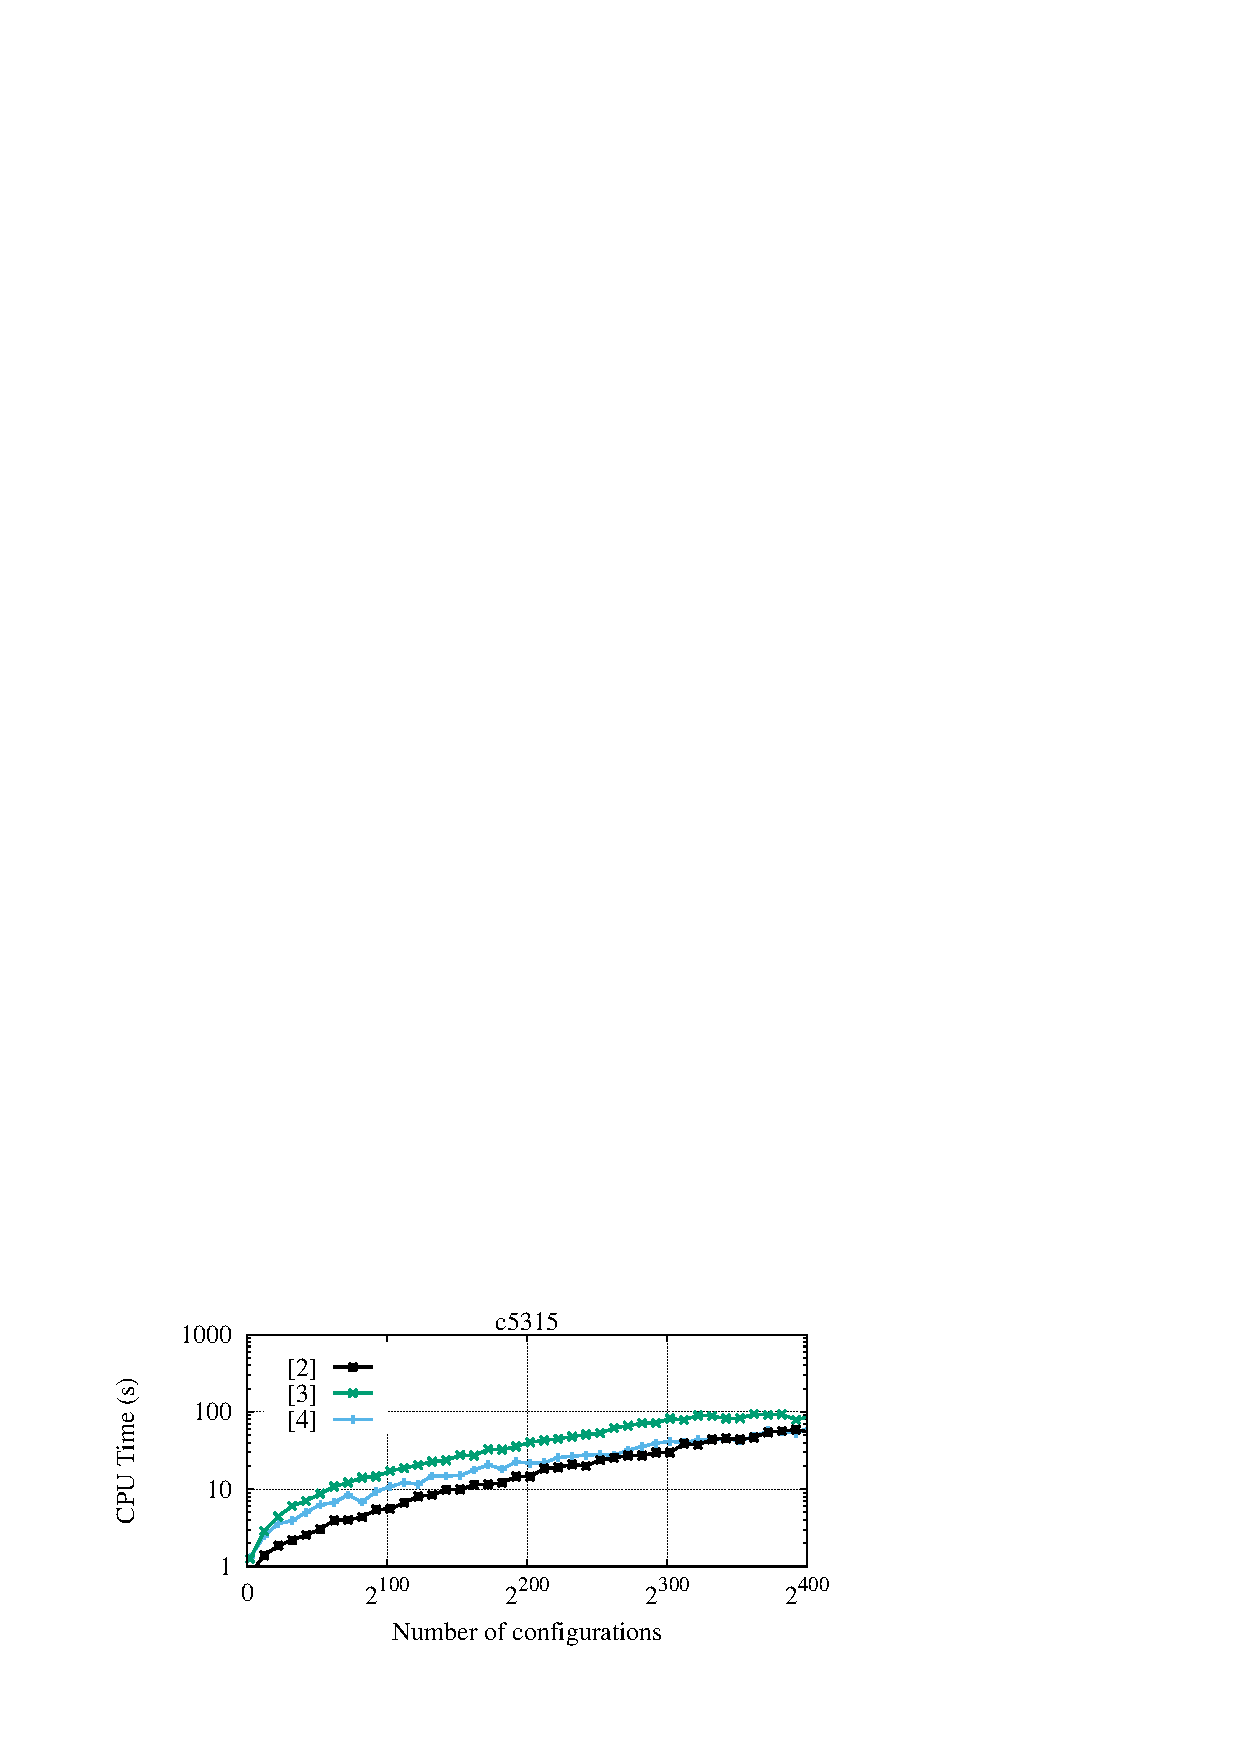
\includegraphics[width=0.48\textwidth]{newdata-tcad16/c5315.pdf} \hspace{.3cm}
    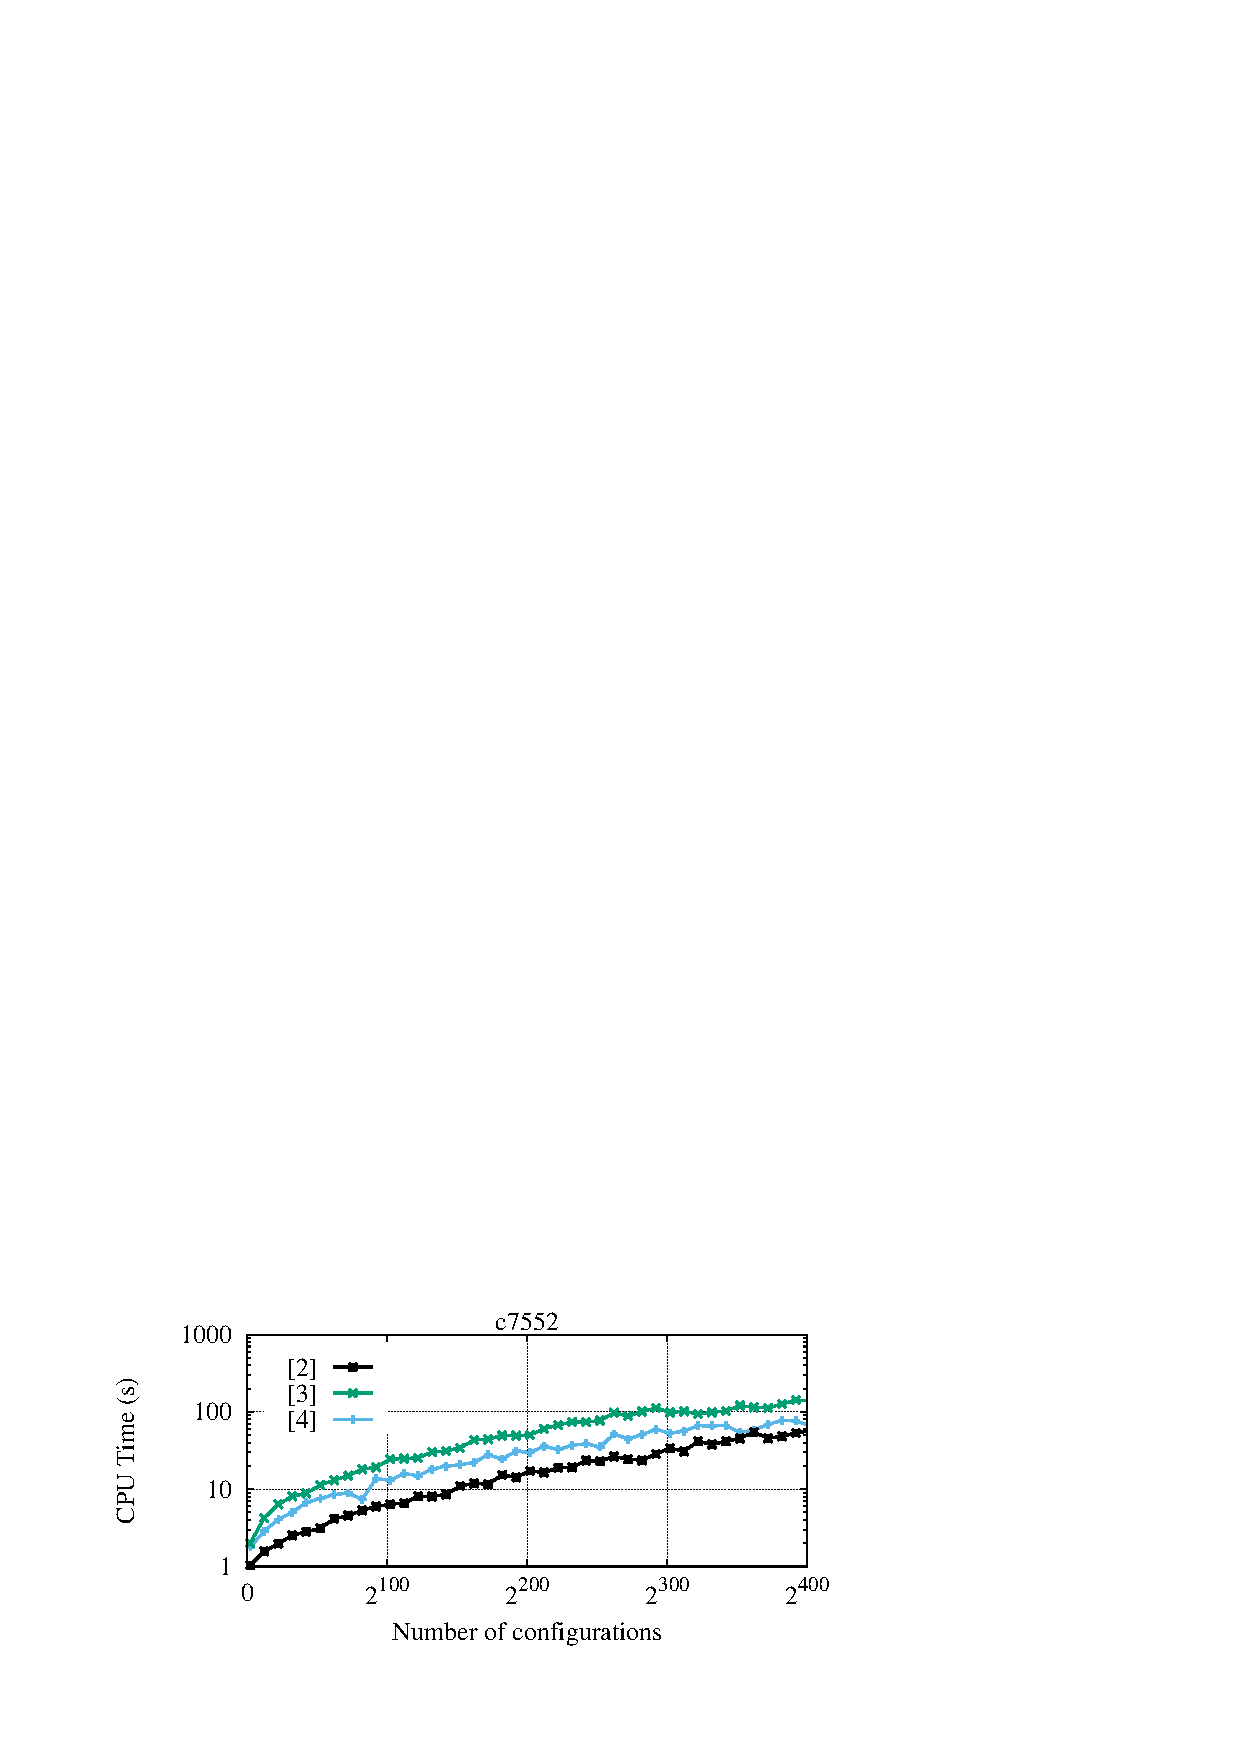
\includegraphics[width=0.48\textwidth]{newdata-tcad16/c7552.pdf}

    \caption{Plots show average runtime to deobfuscate eight ISCAS-85 benchmarks with varied numbers of randomly obfuscated components using the camouflaging techniques presented in {\textit{Camouflaged Standard Cells}\cite{rajendran-13}, \textit{Obfusgates}\cite{malik-obfusgate} and \textit{Transformable Interconnects}\cite{chen-2015-dummyWire}}. Specifically, the runtimes shown are the average runtimes over 10 random trials for each technique and number of obfuscated components.}
    \label{fig:tcad16-comparison}
\end{figure*}
We apply our incremental deobfuscation algorithm to reverse engineer designs camouflaged using \textit{Camouflaged Standard Cells}~\cite{rajendran-13}, \textit{Obfusgates}~\cite{malik-obfusgate}, and \textit{Transformable Interconnects}~\cite{chen-2015-dummyWire}. We implement each of the three camouflaging techniques randomly as summarized in Tab.~\ref{tbl:camouflage_candidates} and described here: 
\begin{itemize}

\item For \textit{Camouflaged Standard Cells}, we select {gates to camouflage by randomly choosing among the } NAND2, NOR2, and XOR2 gates of each benchmark circuit, as these are the types of cells that can be realized by the camouflaged standard cells.

\item For \textit{Obfusgates}, although each NAND4 obfusgate can implement 162 different logical functions, most of the functions do not exist in the ISCAS-85 benchmarks. The gates from the ISCAS benchmarks that can be realized by the NAND4 obfusgates are as shown in Tab.~\ref{tbl:camouflage_candidates}.

\item For \textit{Transformable Interconnects}, we select a net randomly to camouflage, and then add \textit{dummy wires} from three other nets to the chosen net, giving a choice of four possible drivers for the net that the reverse engineer must resolve. If the dummy wires created cycles, then a reverse engineer could identify these wires as dummies from the topological analysis, so when camouflaging a net, we avoid creating dummy wires from any signals in the transitive fanout of that net. 

\end{itemize}



We apply all three techniques to the eight ISCAS benchmarks, as shown in Fig.~\ref{fig:tcad16-comparison}. In each case, we vary the number of components that are obfuscated, and for each number of obfuscated components, we repeat the experiment 10 times making different random choices of which components to obfuscate, and plot the average runtime. To provide a common framework for comparison, we plot the deobfuscation runtime against the number of possible configurations in Fig.~\ref{fig:tcad16-comparison}. The number of possible configurations is $2^x$ where $x$ is the number of programming bits needed to select the functionality of the circuit. {The value of $x$ also indicates the number of camouflaged cells in the circuits. Specifically, in Fig.~\ref{fig:tcad16-comparison}, the numbers of camouflaged cells for \textit{Camouflaged Standard Cells} \cite{rajendran-13}, \textit{Obfusgates} \cite{malik-obfusgate}, and \textit{Transformable Interconnects} \cite{chen-2015-dummyWire} are $x/2$, $x/5$, and $x/2$, respectively} Note that we don't consider here that some programming bits select the same logic function. 

\begin{itemize}

\item For \textit{Camouflaged Standard Cells}, we select {gates to camouflage by randomly choosing among the } NAND2, NOR2, and XOR2 gates of each benchmark circuit, as these are the types of cells that can be realized by the camouflaged standard cells.

\item For \textit{Obfusgates}, although each NAND4 obfusgate can implement 162 different logical functions, most of the functions do not exist in the ISCAS-85 benchmarks. The gates from the ISCAS benchmarks that can be realized by the NAND4 obfusgates are as shown in Tab.~\ref{tbl:camouflage_candidates}.

\item For \textit{Transformable Interconnects}, we select a net randomly to camouflage, and then add \textit{dummy wires} from three other nets to the chosen net, giving a choice of four possible drivers for the net that the reverse engineer must resolve. If the dummy wires created cycles, then a reverse engineer could identify these wires as dummies from the topological analysis, so when camouflaging a net, we avoid creating dummy wires from any signals in the transitive fanout of that net. 

\end{itemize}


\begin{figure*}[!hbt]
  \centering
  {
%  \subfloat[Eliminating feasible configurations using c2670.\label{fig:sharpSAT1}]{%
  \subfloat{%
    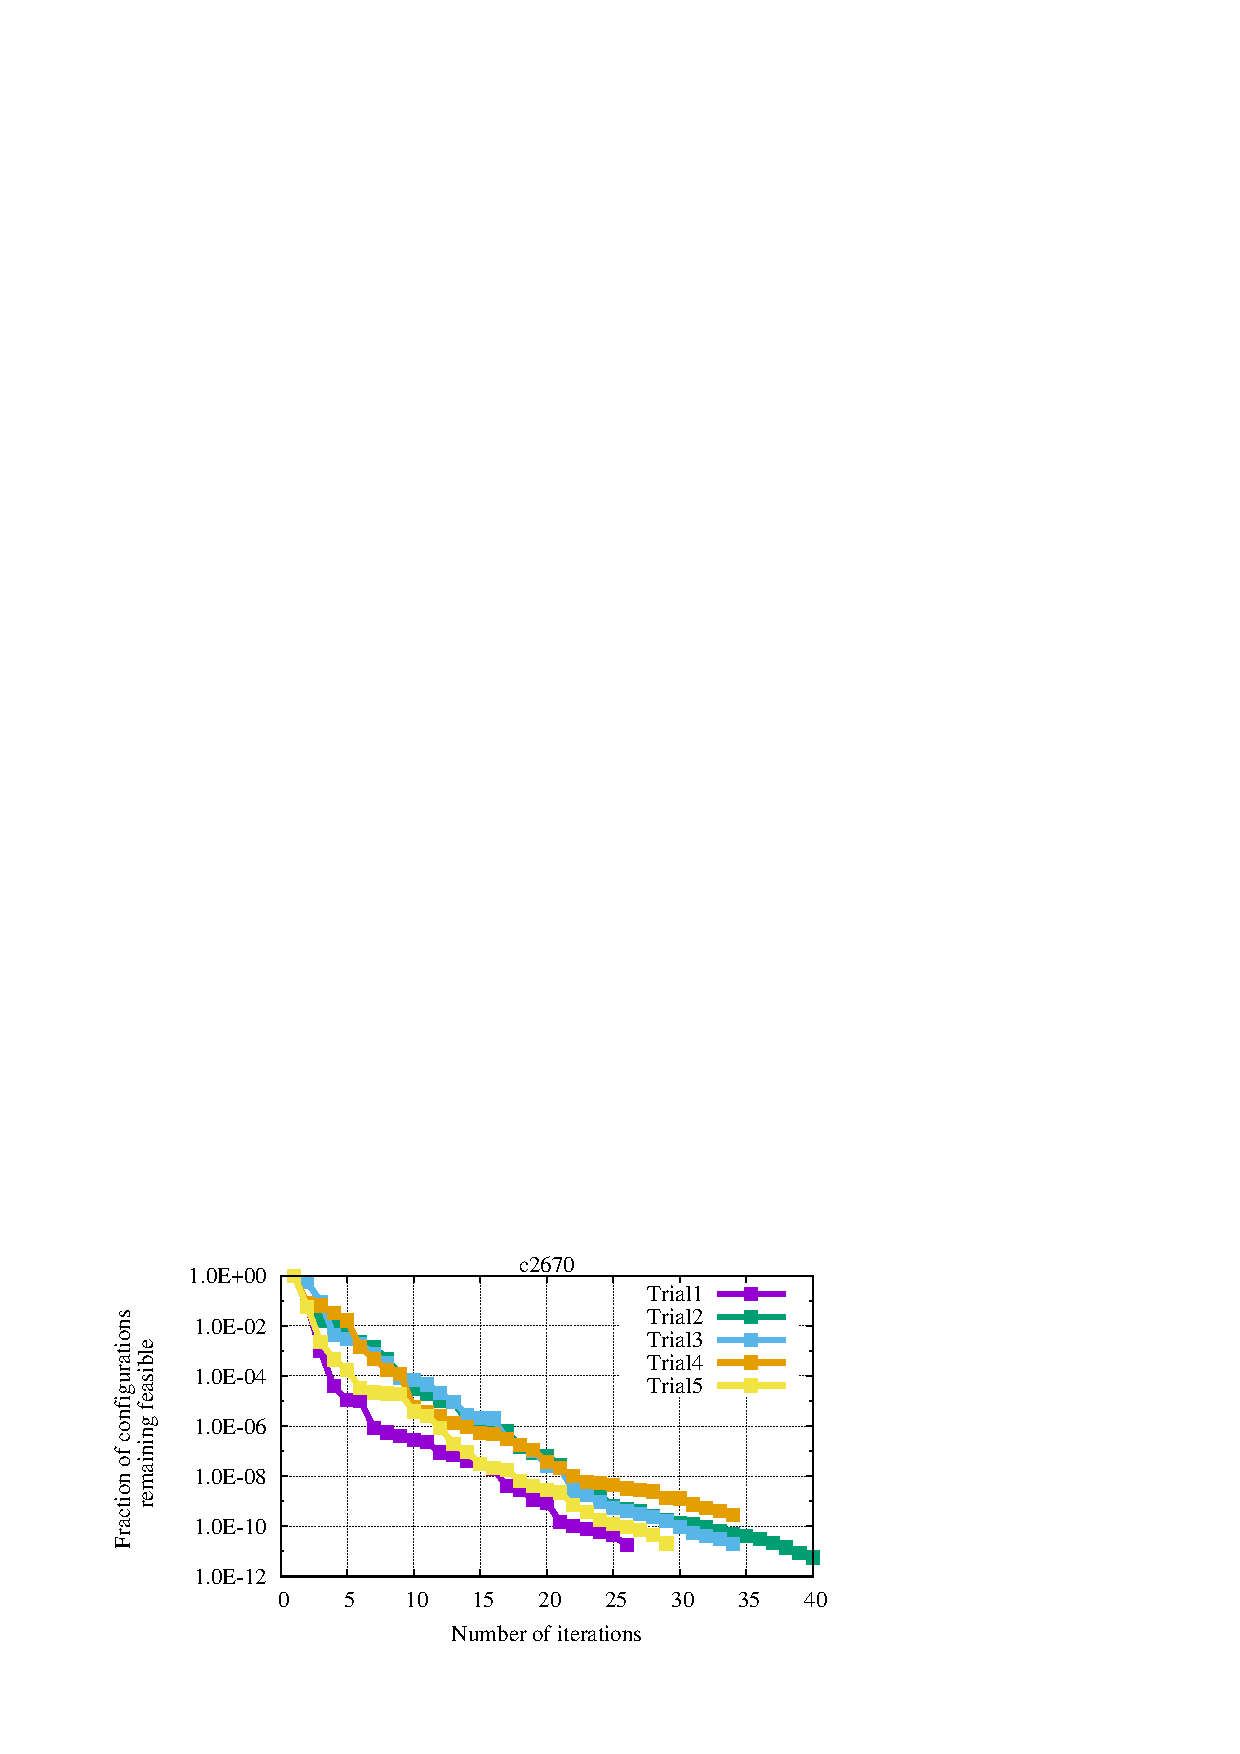
\includegraphics[width=0.45\textwidth]{sharpSAT_scirpt_gnuplot/sharpSAT-c2670.pdf} 
    }
%      \subfloat[Eliminating feasible configurations using c3540. \label{fig:sharpSAT2}]{%
      \subfloat{%
    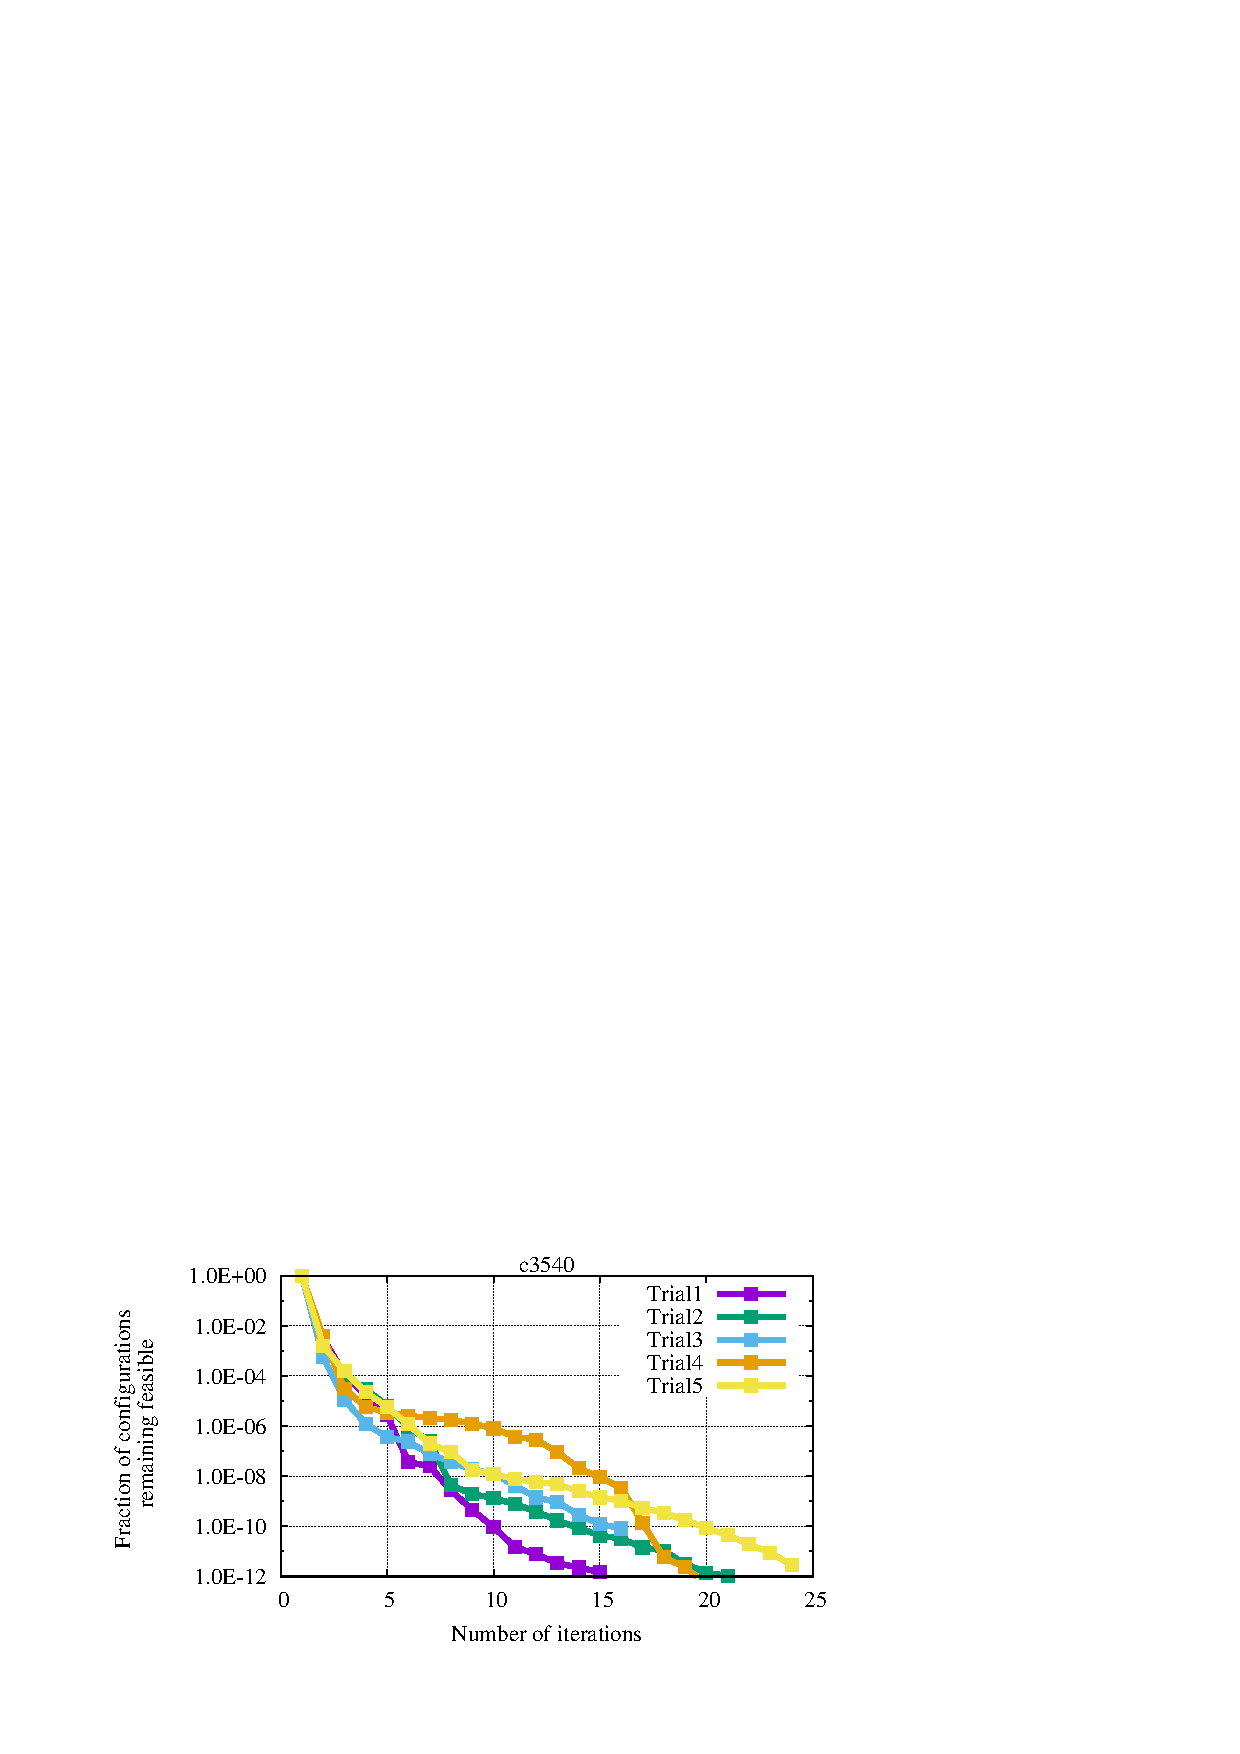
\includegraphics[width=0.45\textwidth]{sharpSAT_scirpt_gnuplot/sharpSAT-c3540.pdf} 
    }
        \vspace{-2mm}
    
        %\subfloat[Eliminating feasible configurations using c5315.\label{fig:sharpSAT3}]{%
      \subfloat{%
    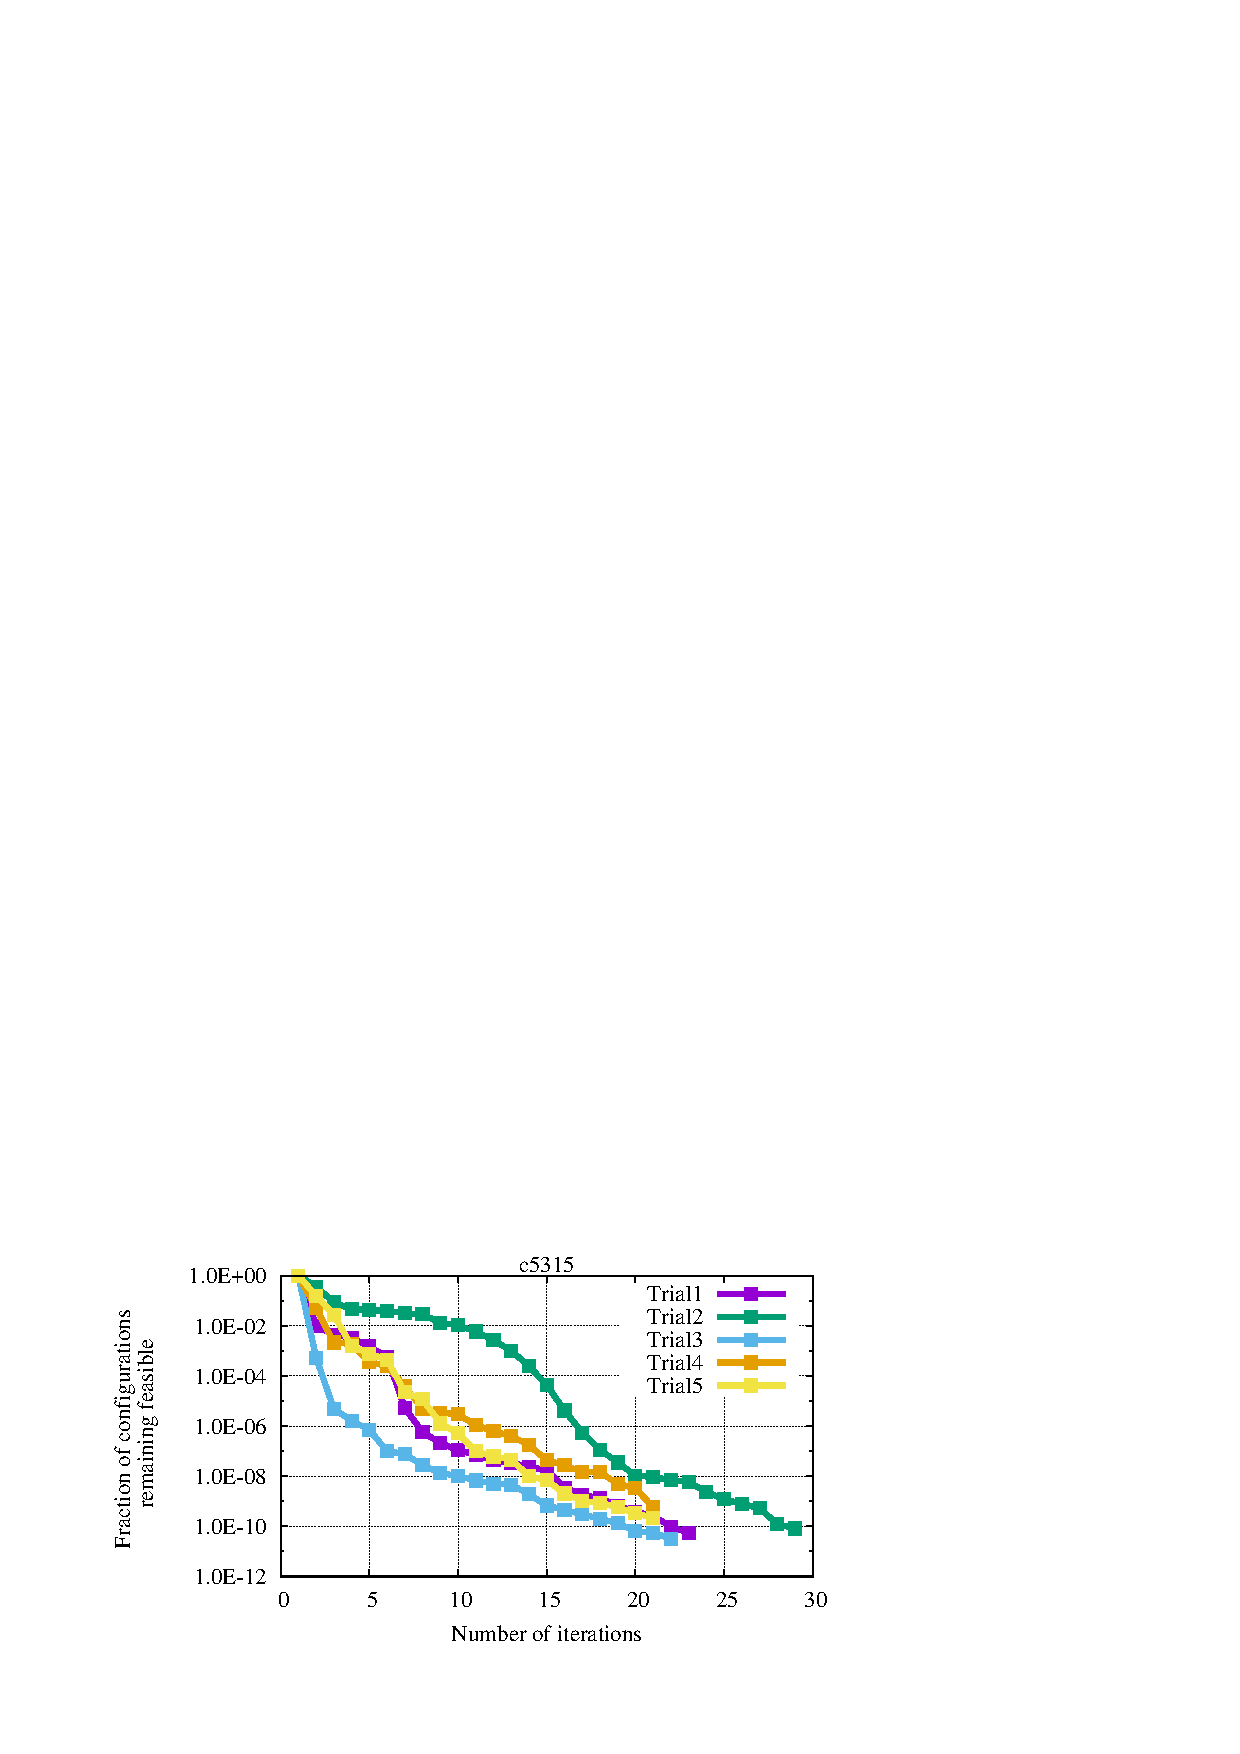
\includegraphics[width=0.45\textwidth]{sharpSAT_scirpt_gnuplot/sharpSAT-c5315.pdf} 
    }
%      \subfloat[Eliminating feasible configurations using c7552. \label{fig:sharpSAT4}]{%
      \subfloat{%
    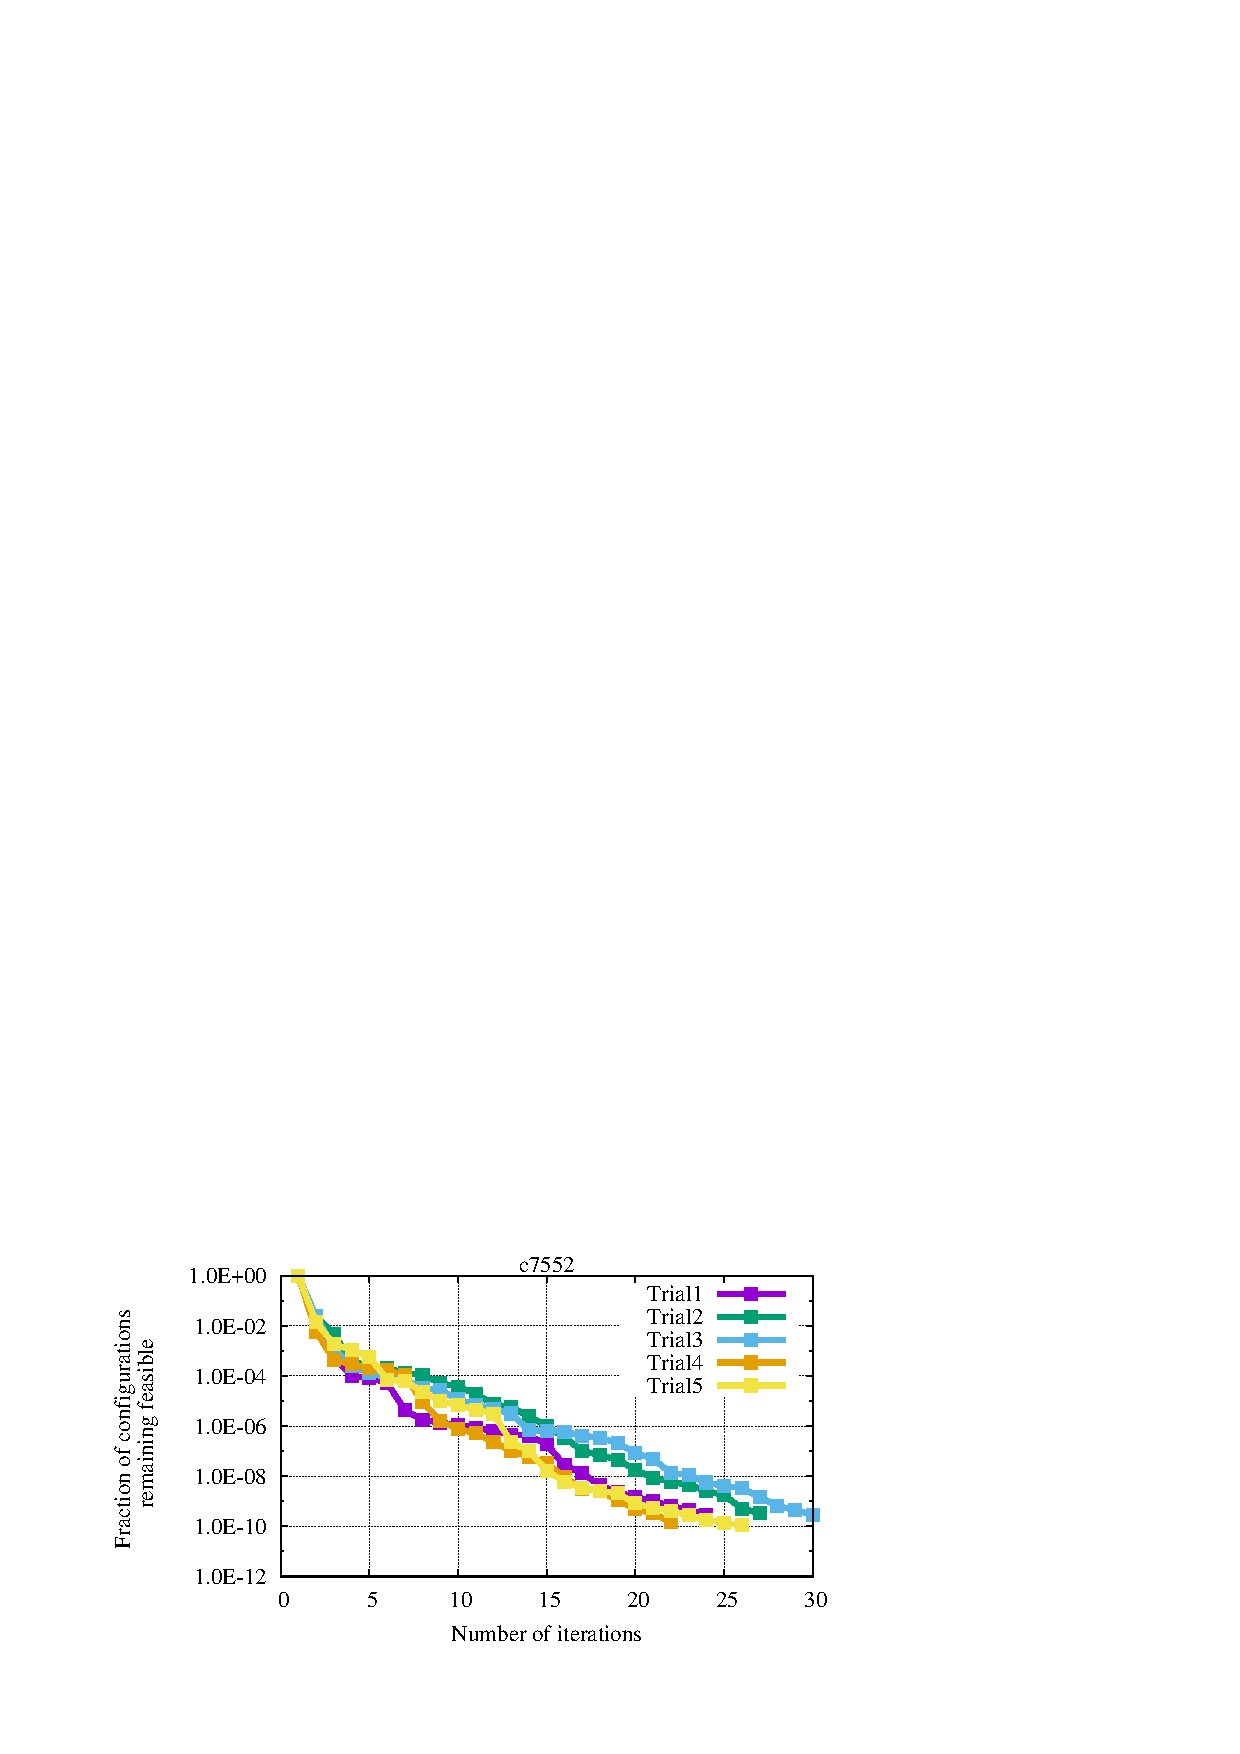
\includegraphics[width=0.45\textwidth]{sharpSAT_scirpt_gnuplot/sharpSAT-c7552.pdf} 
    }
    }
    \vspace{-2mm}
    
    \caption{Eliminating feasible configurations using input-output examples generated by the de-obfuscation algorithm for circuits c2670, c3540, c5315, and c7552 with 51 gates camouflaged using camouflaged standard cells that can implement NAND, NOR or XOR gates. The initial model of each camouflaged circuit has $3^{51}$ configurations. The five trials in each plot denote five different random choices of which gates to camouflage.}
    \vspace{-2mm}
    \label{fig:c7552_coverage}
\end{figure*}


\begin{table}[]
%\normalsize
\centering
\begin{tabular}{|l|c|}
\hline
Camoflaging Technique & \begin{tabular}[c]{@{}c@{}}Camouflagable components\\ in ISCAS-85 benchmarks\end{tabular} \\ \hline
NAND/NOR/XOR camouflaged cells~\cite{rajendran-13} & NAND2, NOR2, XOR2  \\ \hline
%\cite{rajendran-13}* & \begin{tabular}[c]{@{}c@{}}NAND2, NOR2, XOR2,\\ AND2, OR2, XNOR2\end{tabular} & NO \\ \hline
NAND4 Obfusgates~\cite{malik-obfusgate} & \begin{tabular}[c]{@{}c@{}}AND/NAND(2,3,4), INV, \\ OR/NOR(2,3,4), BUFFER\end{tabular} \\ \hline
Tranformable Interconnects~\cite{chen-2015-dummyWire} & any net  \\ \hline
\end{tabular}
\caption{Camouflagable components in the ISCAS-85 benchmarks when applying different camouflaging techniques. Note that, in the case of transformable interconnects, any net can be chosen, but the choice of dummy connections is restricted to avoid creating apparent combinational loops.}
\label{tbl:camouflage_candidates}
\end{table}

    \begin{figure*}[!ht]
  \centering
    \subfloat[Runtime of deobfuscation.\label{subfig:mux2_compare_time}]{%
    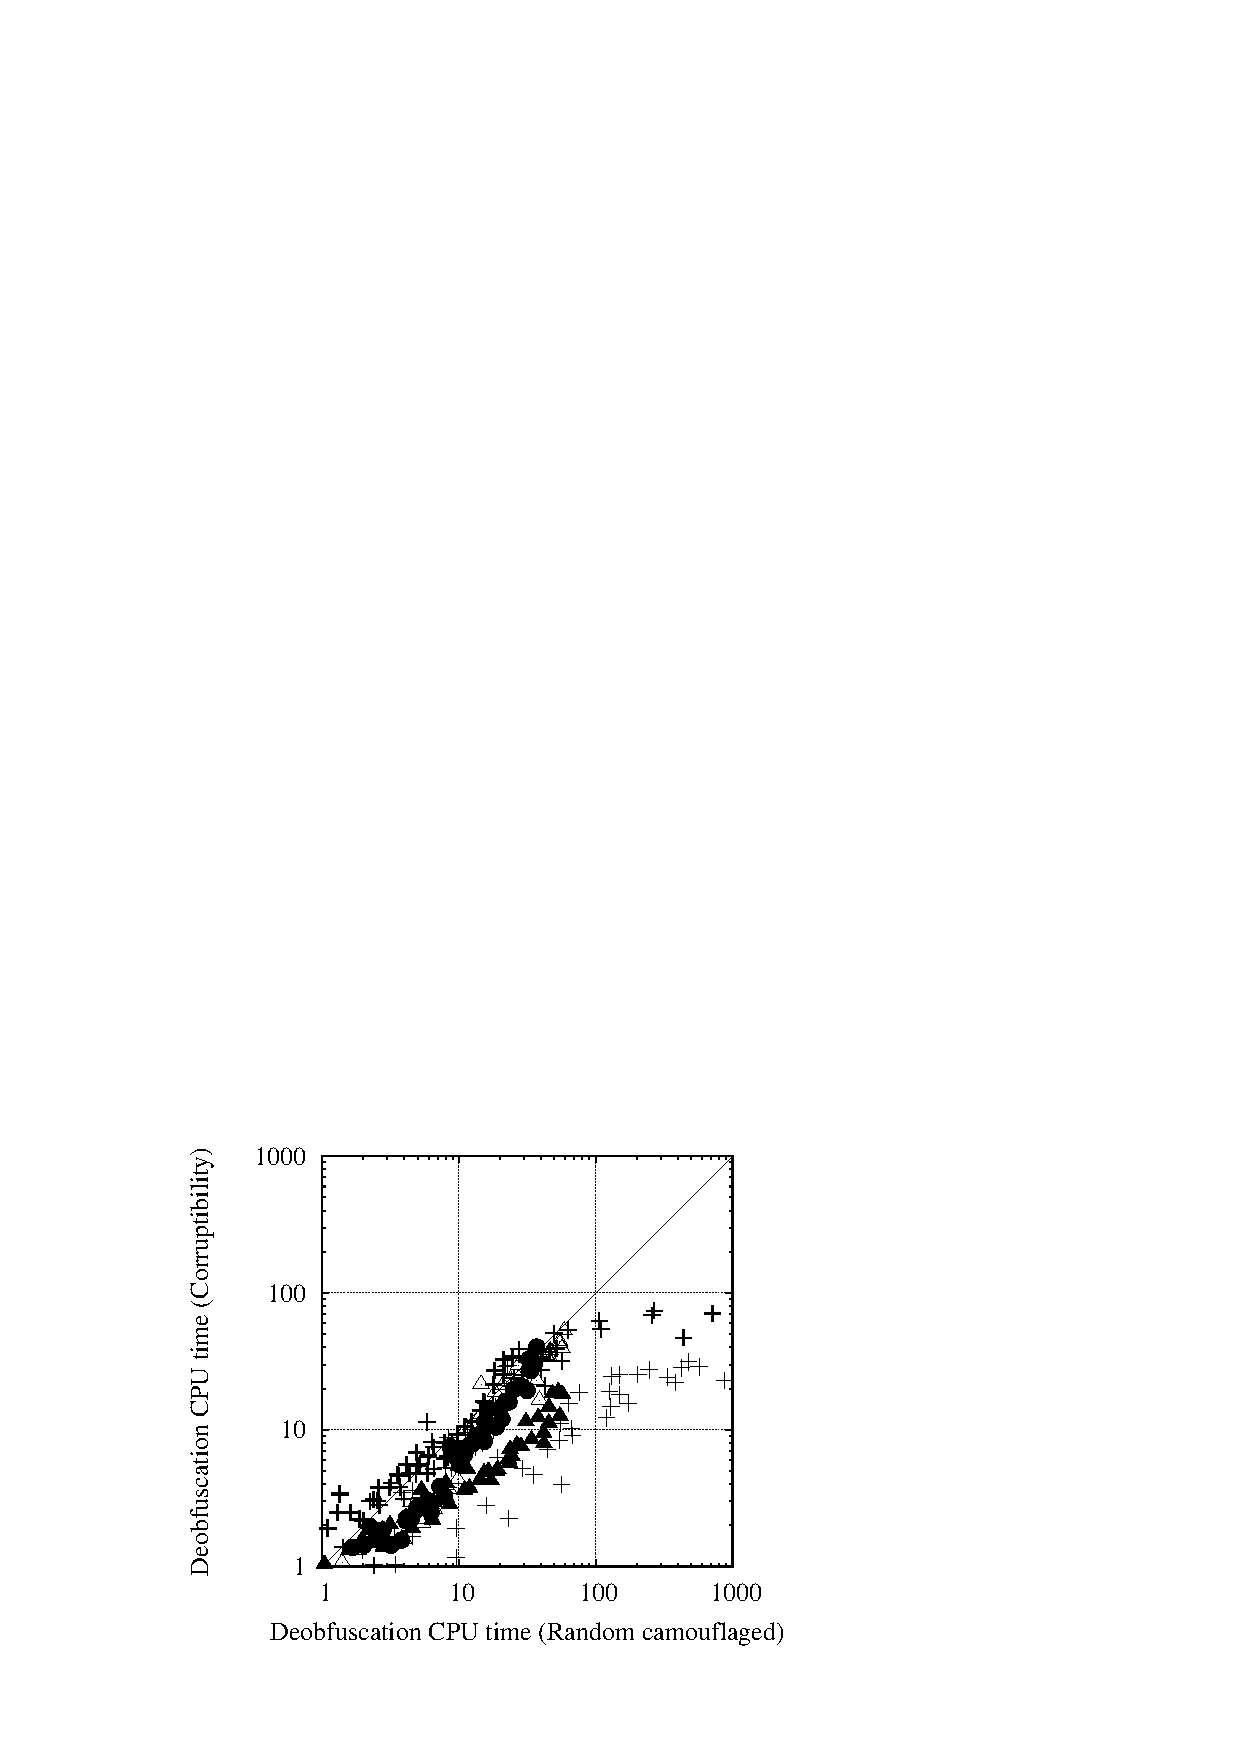
\includegraphics[width=0.4\textwidth]{random_corr/tcad16-mux2-time.pdf} 
    }
    \hspace{20pt}
    \subfloat[Number of vectors of deobfuscation.\label{subfig:mux2_compare_vectors}]{%
    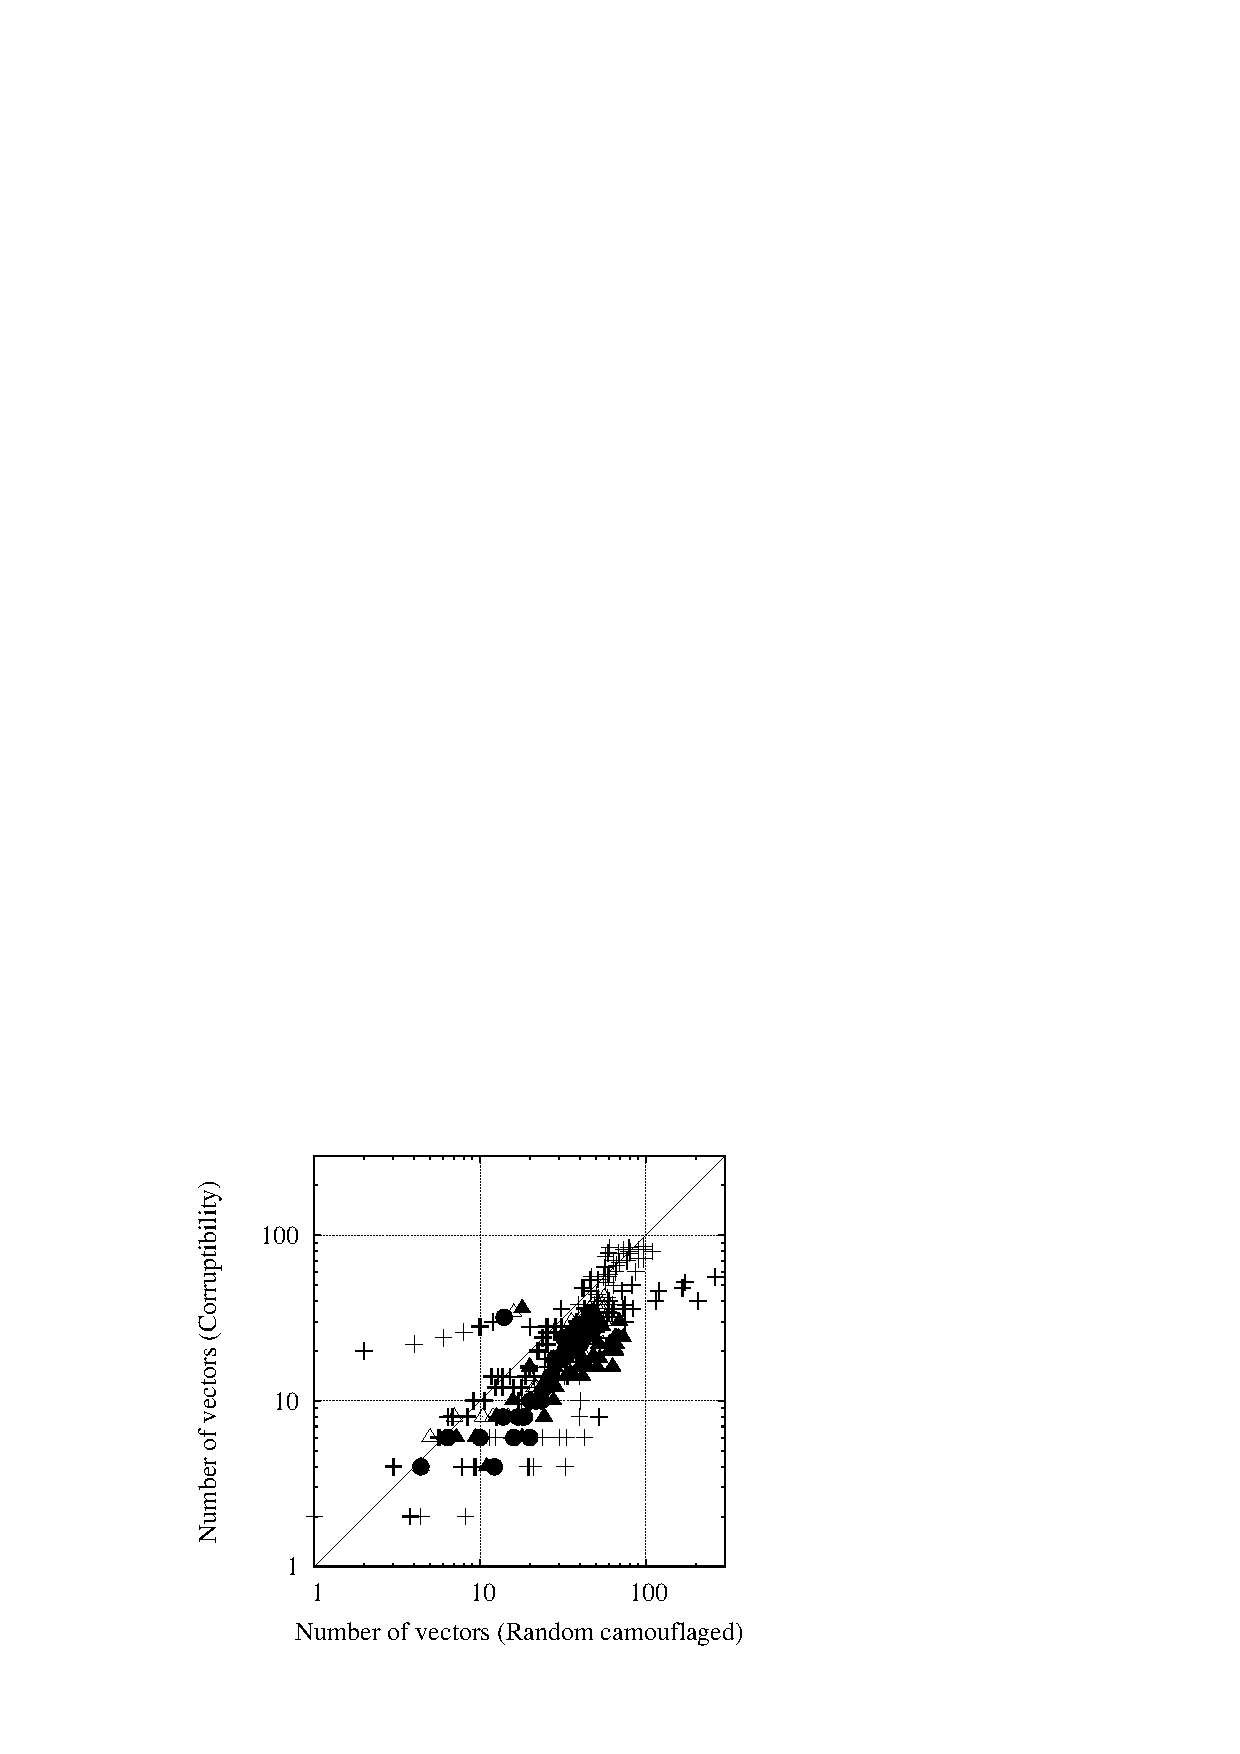
\includegraphics[width=0.4\textwidth]{random_corr/tcad16-mux2-vector.pdf} 
    }
    \caption{Comparing the total deobfuscation CPU time and the number of vectors used for deobfuscation of \textit{Corruptibility}-guided and \textit{random} camouflaged ISCAS-85 benchmarks.}
    \vspace{-2mm}
    \label{fig:comparison_corrupt_random}
  \end{figure*}


%%%%%%%%%%%%%%%%%%%		Quantify				%%%%%%%%%%%%%%%%%%%%%%%%%%
\section{Quantifying the Elimination of Feasible Solutions}
As SAT-based deobfuscation (Alg.~\ref{proc:deobfuscate_incremental}) increasingly rules out infeasible programming vectors representing different possible circuit configurations, we present here a study of how many programming vectors are eliminated at each iteration of the algorithm. Fig.~\ref{fig:c7552_coverage} shows, for circuits c2670, c3540, c5315, and c7552 with \textit{51} camouflaged standard cells, the number of configurations that remain feasible at each iteration of the deobfuscation algorithm. At each iteration, the total number of feasible configurations are obtained by counting the number of satisfying assignments to the CNF-encoded feasibility constraint ($feas(P)$) applied to the programming vector (see line.~\ref{algline:sharpsat} of Alg.~\ref{proc:deobfuscate_incremental}). Note that the number of feasible programming vectors is not counted during normal operation of the deobfuscation algorithm. Counting the number of solutions to a CNF formula is known as the \textit{\#SAT} problem (or as \textit{model counting}~\cite{birnbaum1999good}). The data in Fig.~\ref{fig:c7552_coverage} is obtained using the \#SAT solver sharpSAT~\cite{thurley2006sharpsat}.
















%%%%%%%%%%%%%%%%%%%		Effect				%%%%%%%%%%%%%%%%%%%%%%%%%%
\section{Effect of Corruptibility-based Camouflaging}

As an alternative to randomly selecting gate instances to camouflage, previous works have proposed selecting gates to obfuscate such that incorrect guesses of the camouflaged gates will maximize corruption of the primary outputs~\cite{chakraborty-09,rajendran-13}. When using corruptibility as a metric, a gate is scored for camouflaging according to the average Hamming distance between the output produced under the correct functionality of the gate and an incorrect guess of the gate functionality that could be made by a reverse engineer. We measure corruptibility using the fault simulation tool HOPE~\cite{lee-96}. Since the corruptibility for each circuit is fixed, the camouflaging order is also fixed. The plots Fig.~\ref{fig:comparison_corrupt_random} compares randomly camouflaged circuits and circuits camouflaged according to corruptibility. When camouflaging is chosen to maximize output corruptibility, then any observation of outputs will be highly effective for ruling out large numbers of possible functions of camouflaged components. We notice in Fig.~\ref{fig:comparison_corrupt_random} that 1) corruptibility-guided obfuscation generally requires less CPU time to deobfuscate (Subfig.~\ref{subfig:mux2_compare_time}); 2) corruptibility-guided obfuscation generally requires fewer vectors to deobfuscate each circuit (Subfig.~\ref{subfig:mux2_compare_vectors}). Note, however, that our algorithm does not necessarily minimize the number of vectors.

{The vectors discovered using the SAT-based deobfuscation are not objectively chosen, as they are obtained from satisfying assignments produced by the SAT solver. The vectors may, therefore, be biased by the search heuristics of the solver or other factors. To provide a fairer comparison between random camouflaging and corruptibility-guided camouflaging, we perform experiments using randomly chosen input-output pairings. Instead of using the input-output pairs generated by the SAT solver, we choose input vectors randomly from the space of possible vectors and obtain the corresponding output vectors from the oracle. Each input-output pair is translated to a feasibility constraint, and we again use sharpSAT to count the number of programming vectors that are consistent with the constraints. We repeat this for ten different randomly camouflaged instances of c2670, c3540, c5315 and c7552, and for the same circuits camouflaged according to corruptibility. Figure \ref{fig:random_pi_po_test}, show the average fraction of programming vectors that remain feasible after a single input-output pair. This result shows that a smaller share of configurations remain feasible when using corruptibility-guided camouflaging instead of random camouflaging.}

\begin{figure}[!hbt]
 \centering
 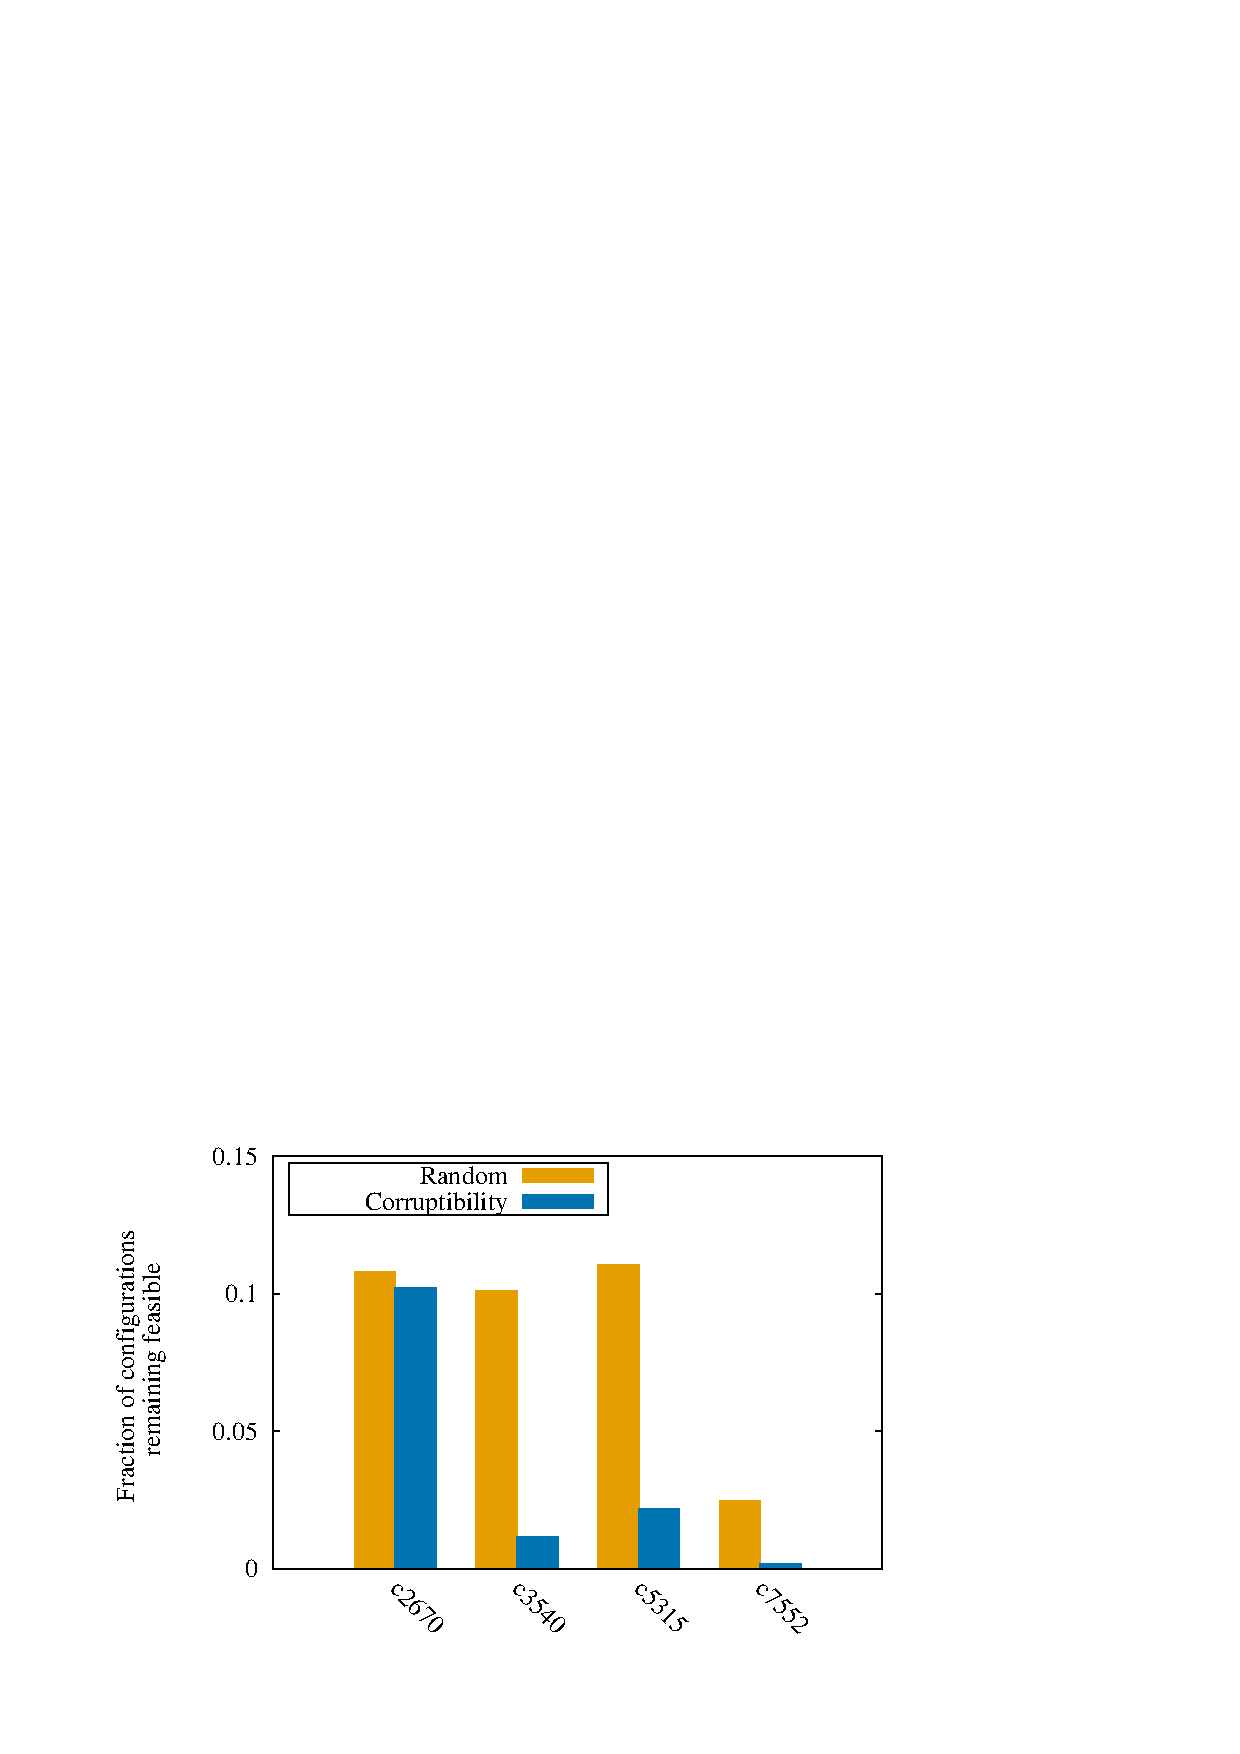
\includegraphics[scale=0.5]{figures/random-pi-po.pdf}
   \caption{Average fraction of configurations that remain feasible with respect to a single randomly-chosen PI-PO pair.}
    \vspace{-2mm}
    \label{fig:random_pi_po_test}
\end{figure}










%%%%%%%%%%%%%%%%%%%		Limitation				%%%%%%%%%%%%%%%%%%%%%%%%%%
\section{Limitation of SAT-based Deobfuscation}

It is well-known that certain circuits, such as multipliers, are particularly challenging for analyzing with SAT~\cite{cook1997finding}, and this limits the effectiveness of SAT-based deobfuscation on such circuits. To examine this, we tested our algorithm on two multipliers. The first is ISCAS-85 benchmark c6288, with ten gates camouflaged using NAND/NOR/XOR camouflaged standard cells. Despite the small number of camouflaged cells, the design required 5.4 hours to deobfuscate. All the iterations except the last one require no more than 2 seconds. The SAT call at the final iteration, because it is the one that returns an UNSAT result (at line~\ref{algline:isat1} of Alg.~\ref{proc:deobfuscate_incremental}), takes many hours. Additionally, we repeat the same experiments on a 16-bit Montgomery multiplier~\cite{koc1998montgomery} in field GF($2^{16}$), and are not able to deobfuscate the multiplier in 6 hours with one gate camouflaged. The reason is that solving GF multiplier problems using SAT is very difficult, which has been studied in \cite{lv2012efficient}. In conclusion, any SAT-based algorithm such as ours will be limited when trying to reverse engineer designs such as multipliers, or cryptographic ciphers, that are notoriously hard for SAT. This fact may be exploited in future works where camouflaging can be deployed in a way that will resist SAT-based reverse engineering~\cite{yasin-15}.

{The problem of logic locking is closely related to the problem of camouflaging~\cite{yasin-transforming}, and in logic locking, recent works show the importance of trying to thwart SAT attacks by ensuring that each input-output example provides limited information about the values of the key bits that unlock the circuit~\cite{yasin2016sarlock}~\cite{xie2016mitigatingsat}. In an extreme case, one can guarantee that an exponential number of input-output examples are needed to exactly learn the key bits, but a consequence of this is that output corruption under incorrect key guesses will be limited~\cite{yasin2016sarlock}. A similar approach has been used with camouflaging to quantify the security of the camouflaged circuits \cite{Yasin-iccad-16} \cite{MengLi-iccad-16}.  Note that in logic locking, care must be taken to ensure that the key gates cannot be identified and removed, and thus to remain secure under reverse engineering logic locking can be combined with obfuscation~\cite{yasin2016sarlock} \cite{shahzad-date17}}. 


\begin{figure}[!hbt]
  \centering
   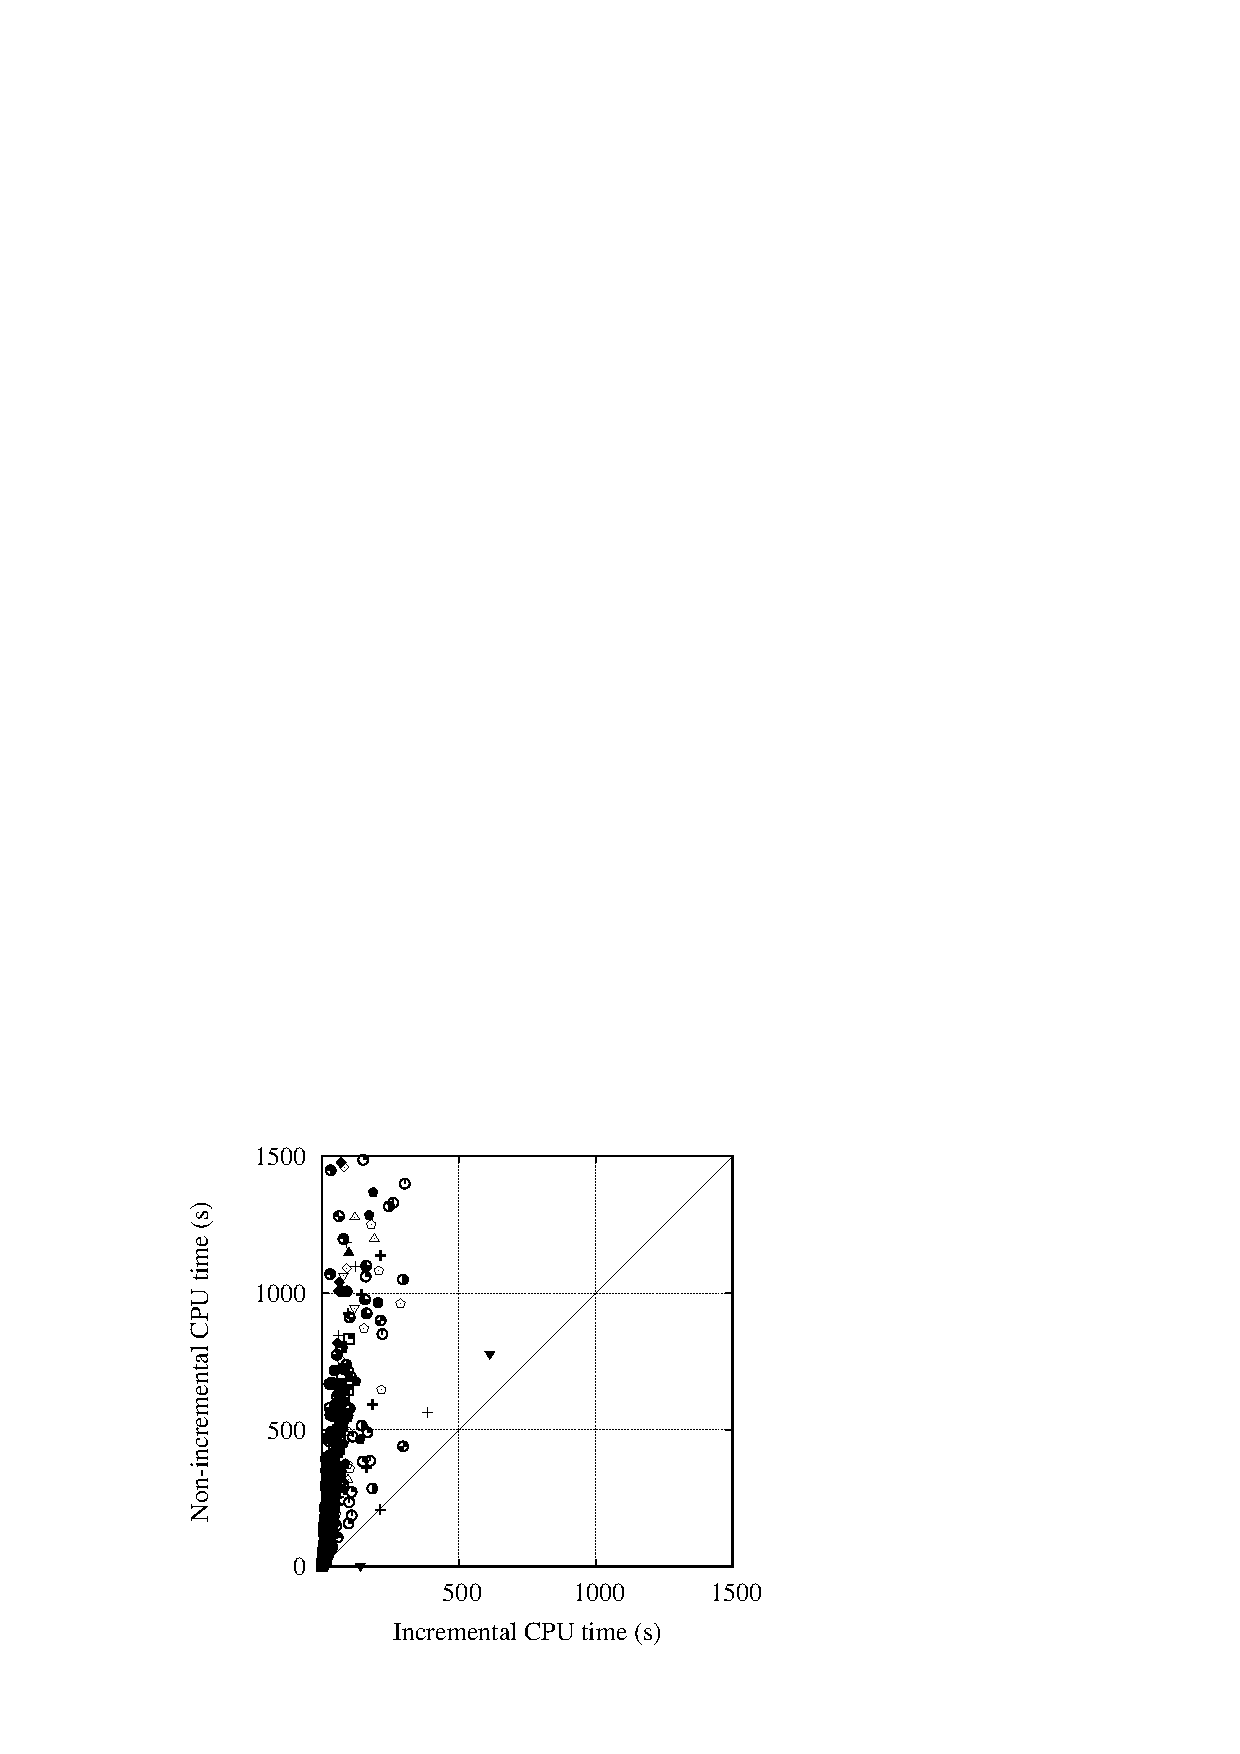
\includegraphics[width=0.45\textwidth]{newdata-tcad16/incre_vs_baseline.pdf} 
    \caption{Comparing the total deobfuscation runtime of baseline and incremental algorithms on 2400 randomly camouflaged circuits instances using different styles of camouflaged gates. The incremental solver gives an average speedup of 10.5x. Runtimes exceeding 1500 seconds are truncated from the plot.}
        \vspace{-2mm}
    \label{fig:incre_vs_baseline}
  \end{figure}

\begin{figure*}[!ht]
  \centering
    \subfloat[Number of clauses remaining in each iteration.\label{subfig:mux2_clauses}]{%
    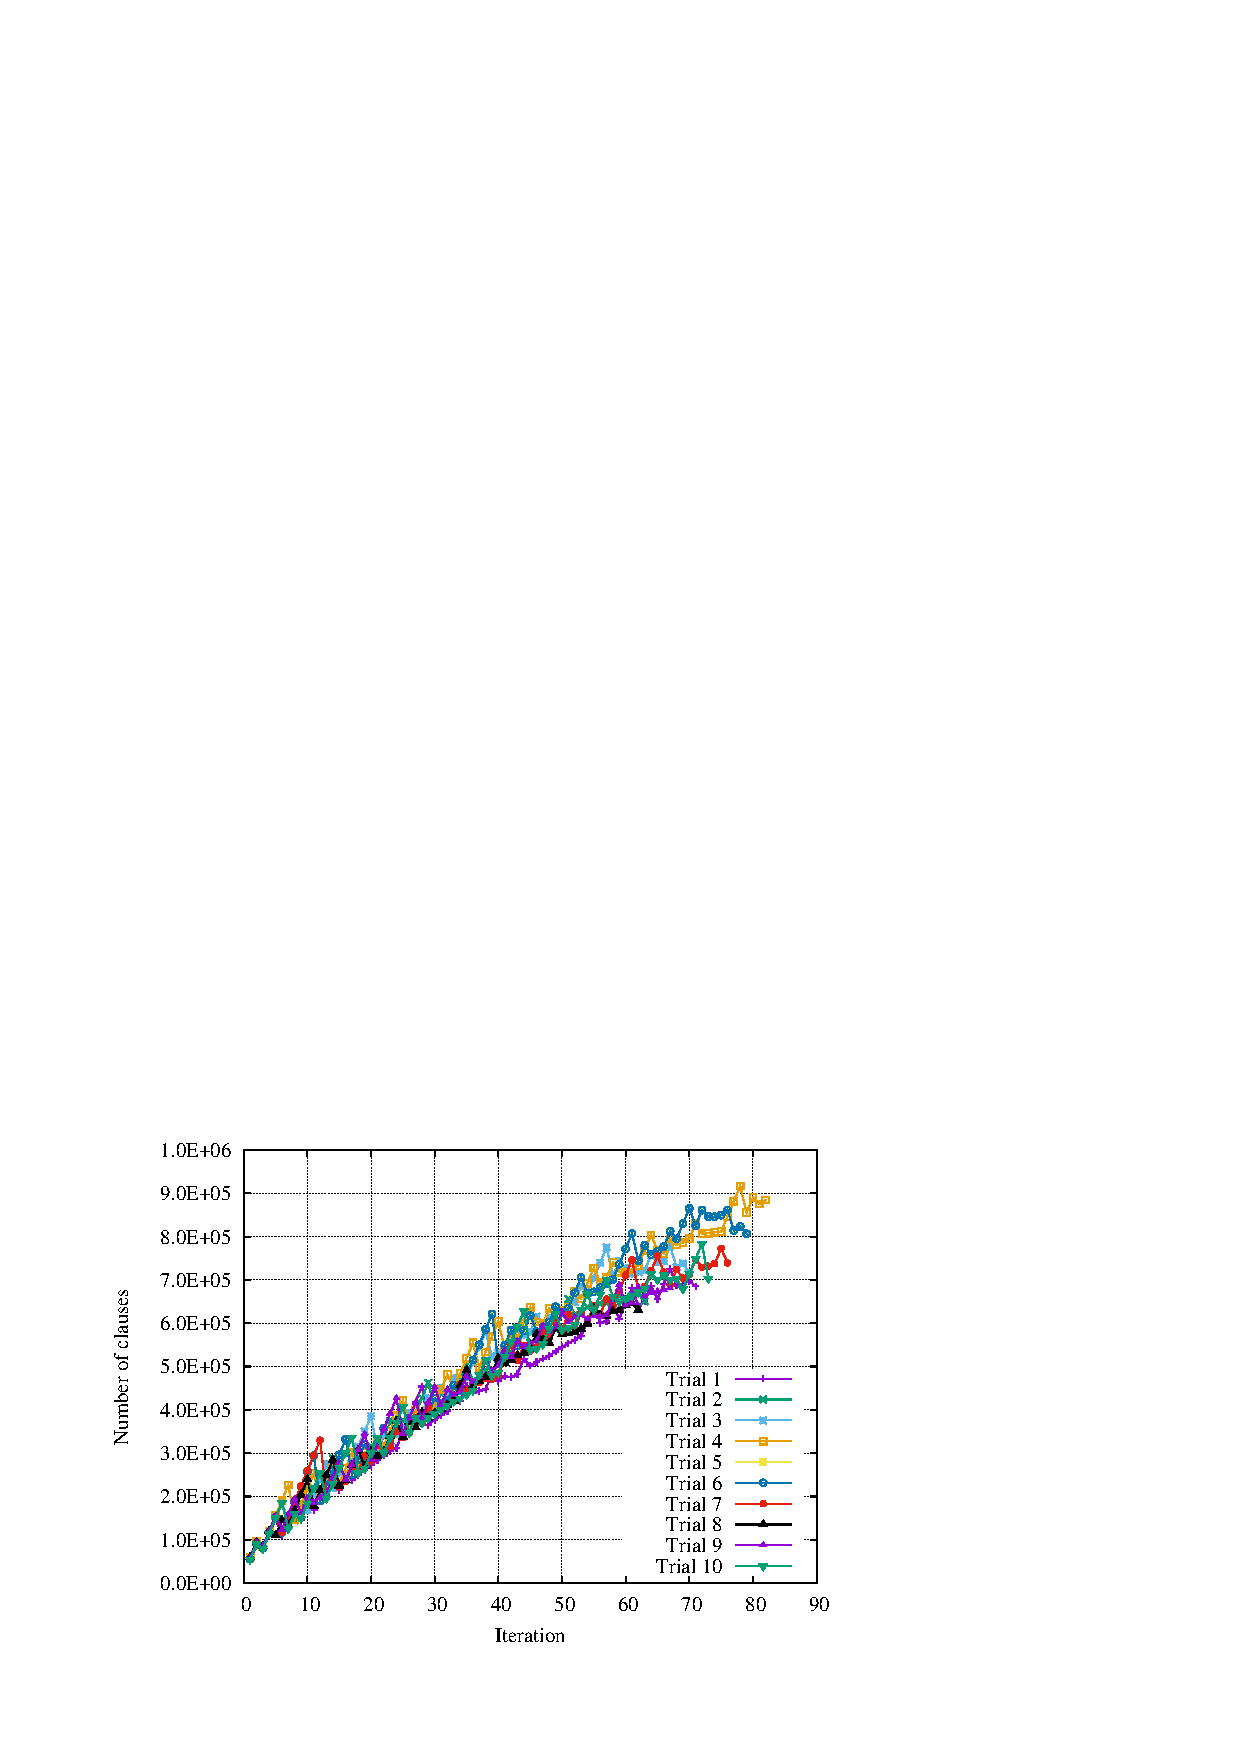
\includegraphics[width=0.42\textwidth]{sharpSAT_scirpt_gnuplot/c7552-clausesNum-10random.pdf} 
    }
    \hspace{20pt}
    \subfloat[Number of non-resolved variables in each iteration.\label{subfig:mux2_vars}]{%
    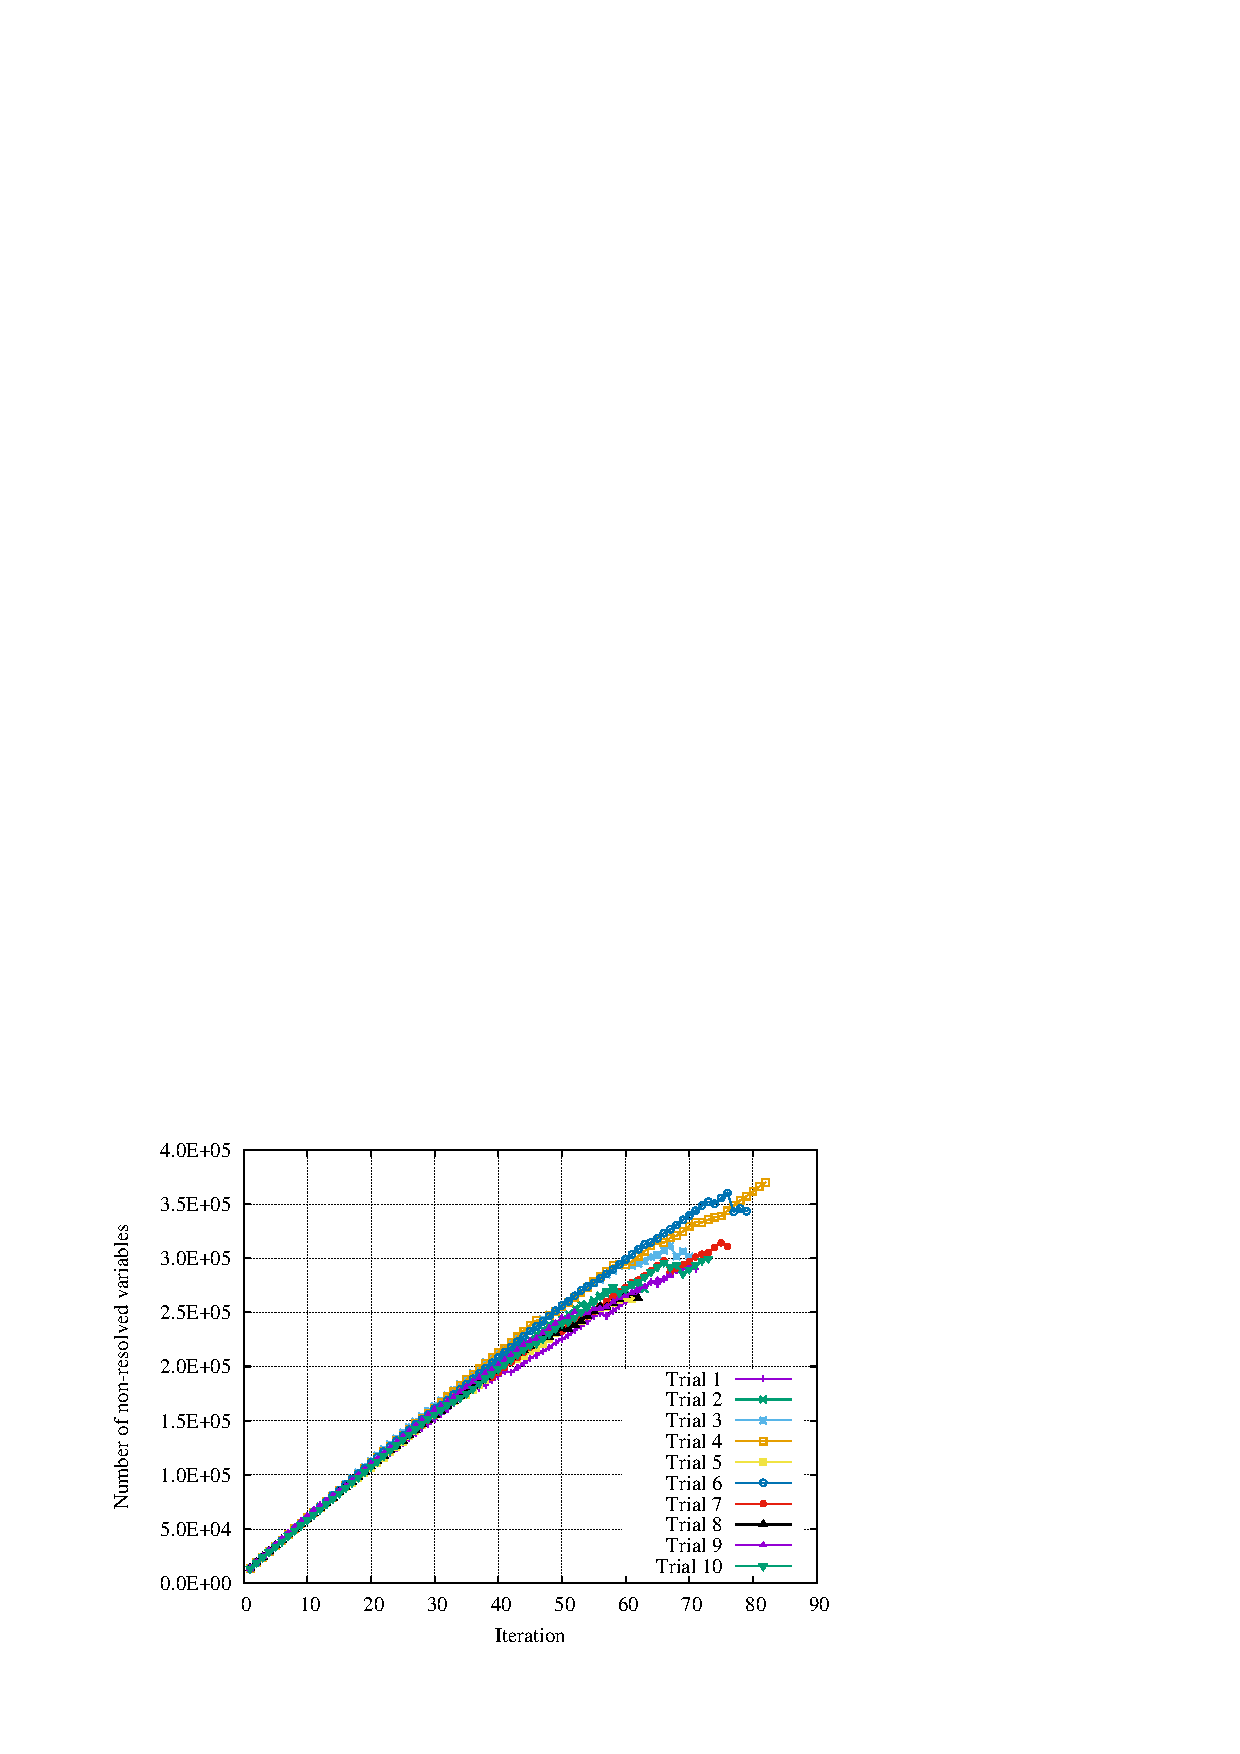
\includegraphics[width=0.42\textwidth]{sharpSAT_scirpt_gnuplot/c7552-varNum-10random.pdf} 
    }
    \caption{Examining the variable and clauses elimination using incremental SAT solving on 10 randomly camouflaged instances of ISCAS-85 benchmark c7552, each with 200 NAND/NOR/XOR camouflaged standard cells~\cite{rajendran-13}.}
    \vspace{-2mm}
    \label{fig:study_incremental}
  \end{figure*}
















%%%%%%%%%%%%%%%%%%%		Incremental				%%%%%%%%%%%%%%%%%%%%%%%%%%
\section{Incremental Algorithm versus Baseline}

We compare the runtimes of our incremental algorithm against a baseline result from our own reimplementation of the algorithm of El Massad et al.~\cite{elmassad-15}, which is the best result demonstrated before ours. {Any style of camouflaging that can be attacked by the incremental SAT algorithm can also be attacked by the baseline algorithm, but our comparison of the two focuses } on \textit{Camouflaged Standard Cells} because this is the technique deobfuscated in El Massad's work.
 Fig.~\ref{fig:incre_vs_baseline} shows the runtime using baseline and incremental algorithms to deobfuscate ISCAS-85 benchmarks with randomly selected gates that use the NAND/NOR/XOR camouflaged standard cells and the cells from Fig.~\ref{subfig:select4}. The position of each datapoint indicates its runtime for the incremental solver and runtime for the baseline solver. {The incremental solver gives a 10.5x reduction in average runtime across all examples compared to the baseline approach, and the average speedup is 6.5x; the difference between the two metrics is that average runtime is strongly influenced by the largest examples, where the incremental solver gives a larger improvement. While our result does not challenge the complexity results established by El Massad for the baseline algorithm, we do show that a significant performance improvement is possible using incremental SAT.}

%While the use of incremental SAT gives a speedup over the baseline algorithm, the class of problems that can be solved with the two approaches are the same. problem



To understand the efficiency of the incremental algorithm, we study in more detail the incremental deobfuscation of circuit c7552 with 200 gates camouflaged using the NAND/NOR/XOR style~\cite{rajendran-13}. Fig.~\ref{fig:study_incremental} shows how the number of clauses and unresolved variables grow as the incremental algorithm proceeds. If the solver is not able to make any simplifications, then both clauses and unresolved variables will grow linearly with the number of iterations as new copies of the CNF-encoded circuit are added to the problem. Subfig.~\ref{subfig:mux2_clauses} shows sub-linear growth in the number of clauses in each iteration of the incremental algorithm, and Subfig.~\ref{subfig:mux2_vars} shows sub-linear growth in the number of unresolved variables. This indicates that partial information from different copies of the circuit CNF are being combined in useful ways. 

\chapter{CONCLUSION}

This paper proposes an incremental-SAT based approach for deobfuscating camouflaged circuits. We have implemented the algorithm and tested its performance by using it to deobfuscate ISCAS-85 combinational benchmarks when camouflaged using three different styles of component camouflaging. The results show that our algorithm is able to efficiently deobfuscate the ISCAS-85 benchmarks regardless of camouflaging style, and are able to do so 10.5x faster than the best existing approaches. Our tool is released publicly to evaluate and support development of future selective component camouflaging approaches. 

%% End of body
%%%%%%%%%%%%%%%%%%%%%%%%%%%%%%%%%%%%%%%%%%%%%%%%%%%%%%%%%%%%%%%%%%%%%%%%%%%%%%%

\appendix
\chapter{THE FIRST APPENDIX TITLE}
...
\chapter{THE SECOND APPENDIX TITLE}
...

%%
%% Beginning of back matter
\backmatter  %% <--- mandatory

%%
%% We don't support endnotes

%%
%% A bibliography is required.
\interlinepenalty=10000  % prevent split bibliography entries
\bibliographystyle{umassthesis}
\bibliography{proposal}
\end{document}

%%% Local Variables: 
%%% mode: latex
%%% TeX-master: t
%%% End: 
